\chapter{\texorpdfstring{\QCDjets and \wjets}{QCD multi-jet and W+Jets} Background Fits}
\label{app:qcd_fits}

\begin{figure}[!htbp]
    \centering
    \begin{subfigure}[b]{\SideBySidePlotWidth}
        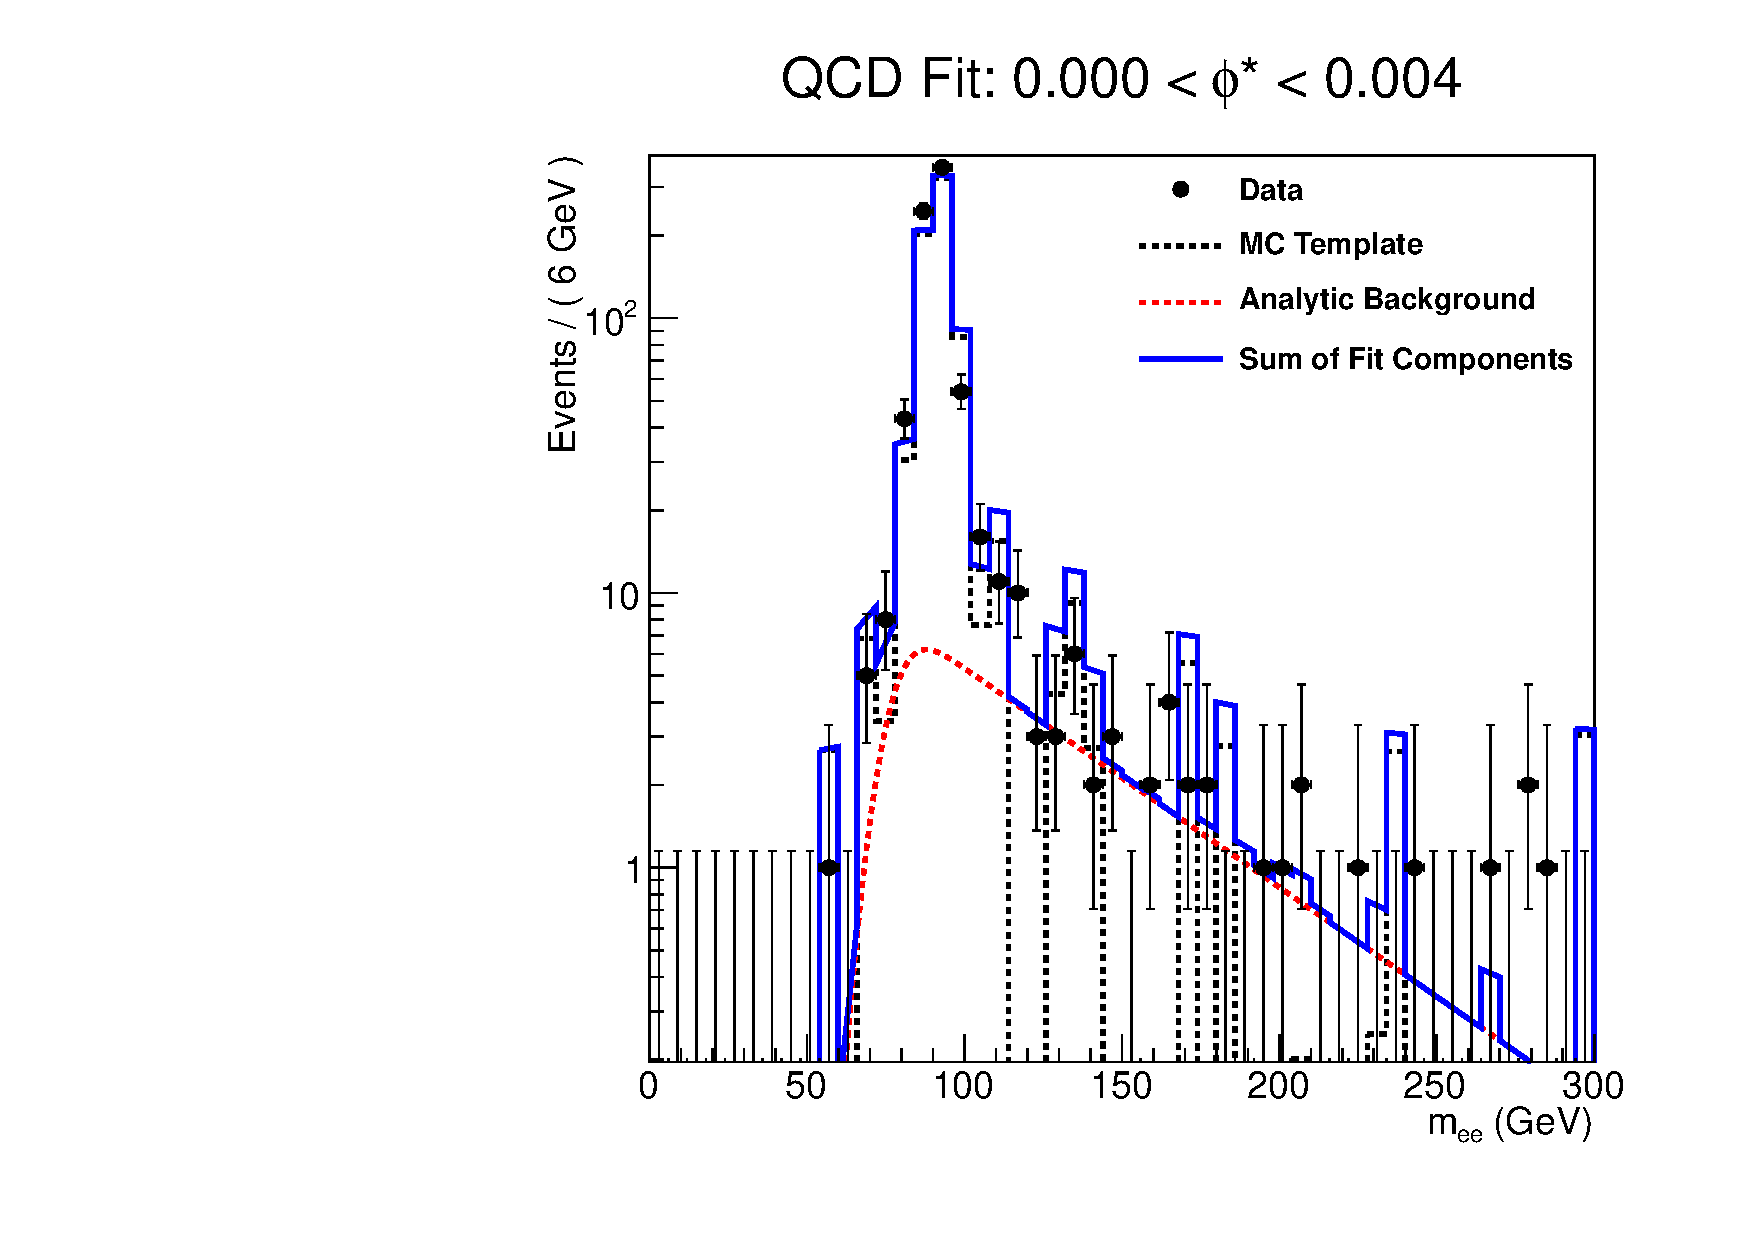
\includegraphics[width=\linewidth]{figures/qcd_fits/qcd_fit_plot_for_01.pdf}
        \label{fig:qcd_fit_01}
    \end{subfigure}%
    % The comment right after suppresses white space that would push the images
    % to new lines
    \begin{subfigure}[b]{\SideBySidePlotWidth}
        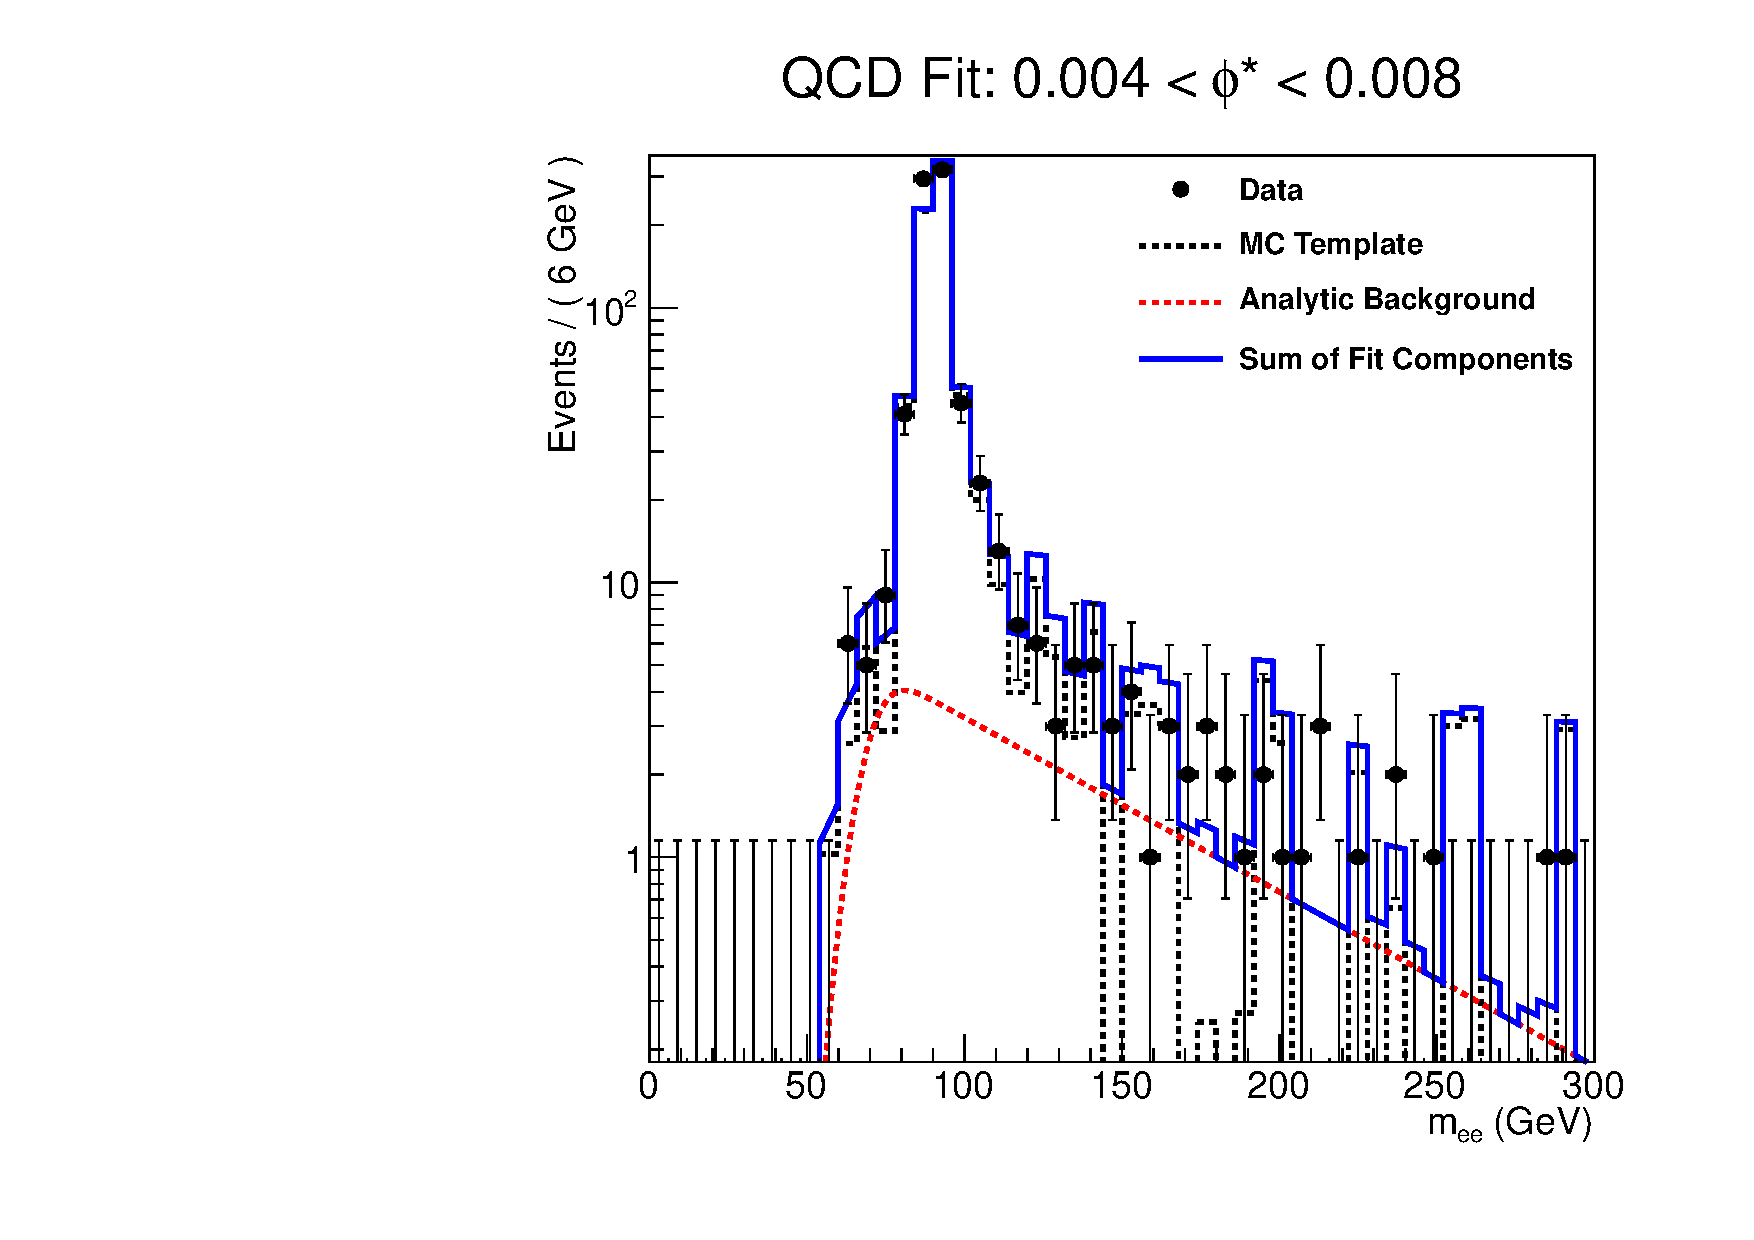
\includegraphics[width=\linewidth]{figures/qcd_fits/qcd_fit_plot_for_02.pdf}
        \label{fig:qcd_fit_02}
    \end{subfigure}
    % New line
    \begin{subfigure}[b]{\SideBySidePlotWidth}
        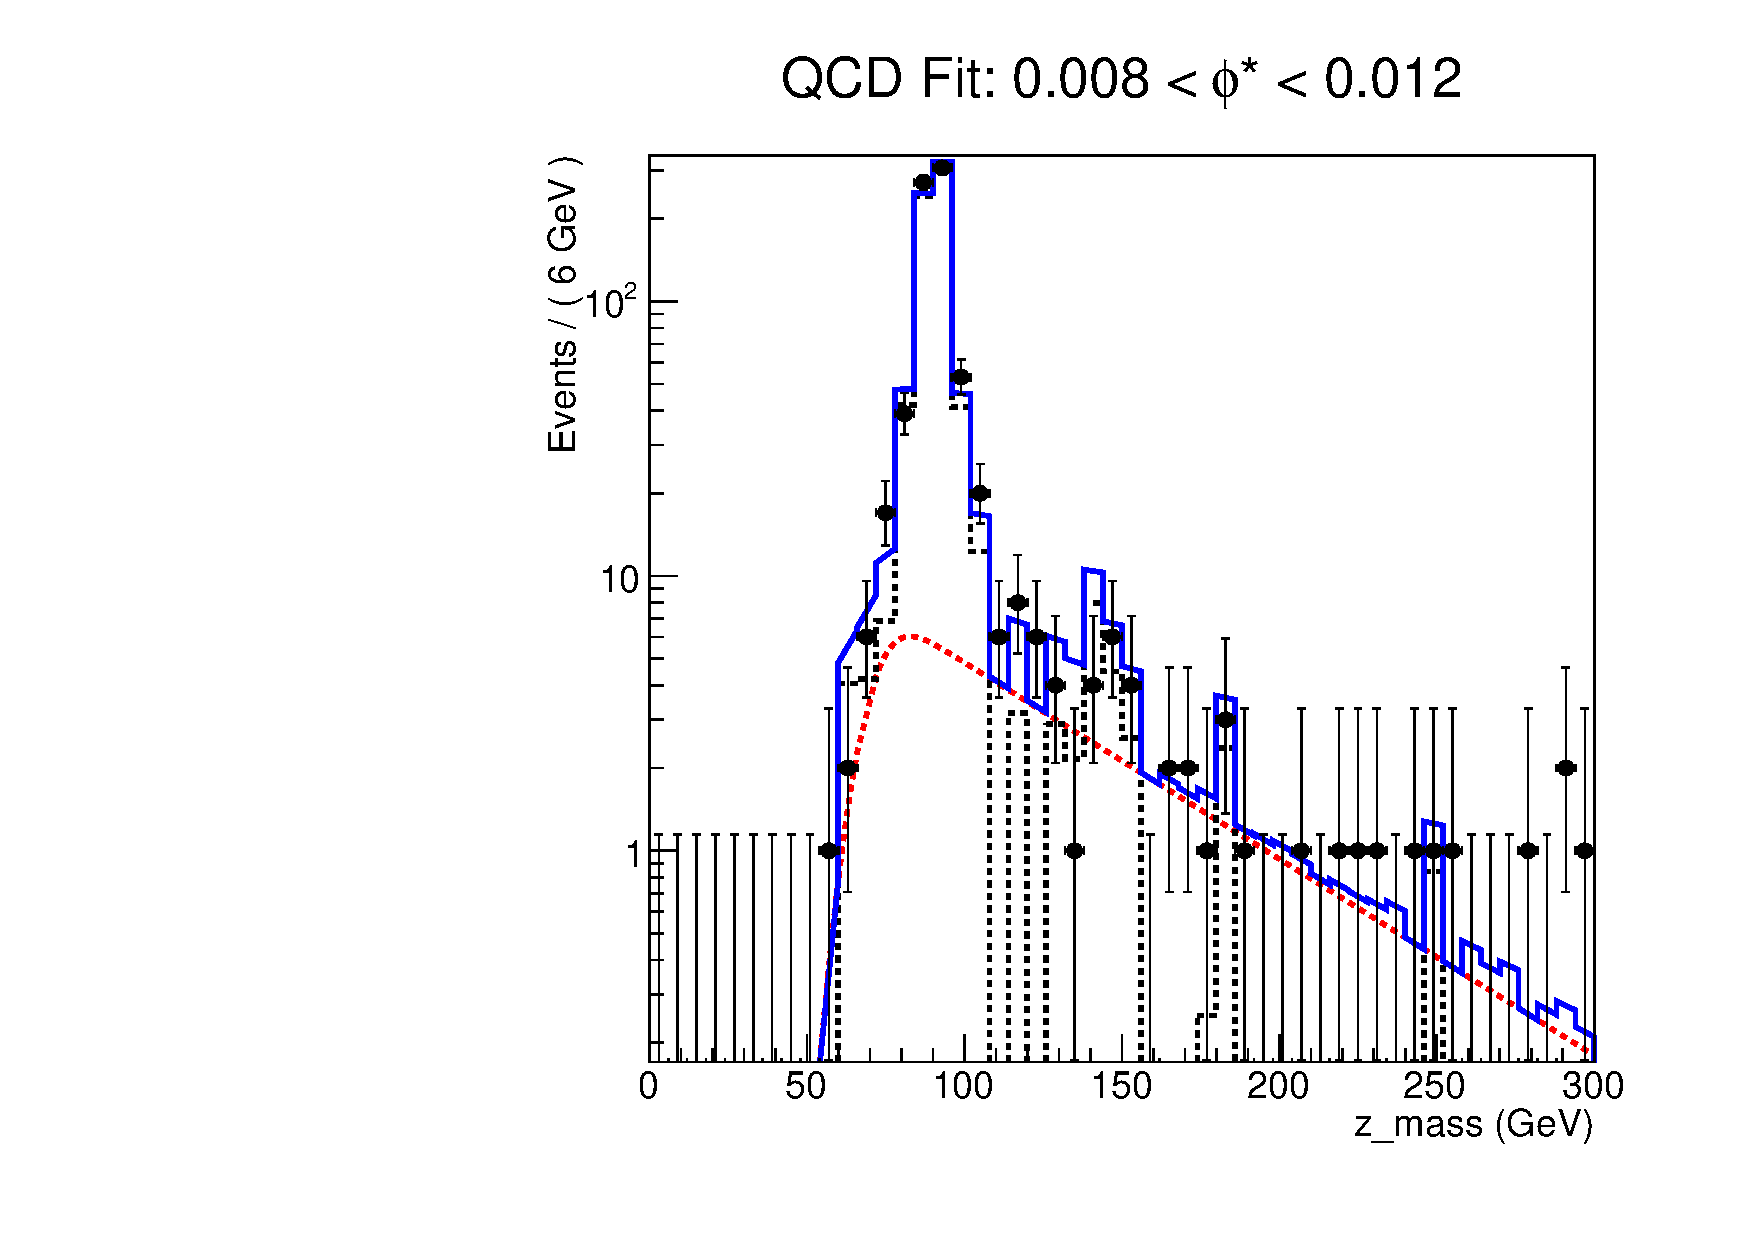
\includegraphics[width=\linewidth]{figures/qcd_fits/qcd_fit_plot_for_03.pdf}
        \label{fig:qcd_fit_03}
    \end{subfigure}%
    \begin{subfigure}[b]{\SideBySidePlotWidth}
        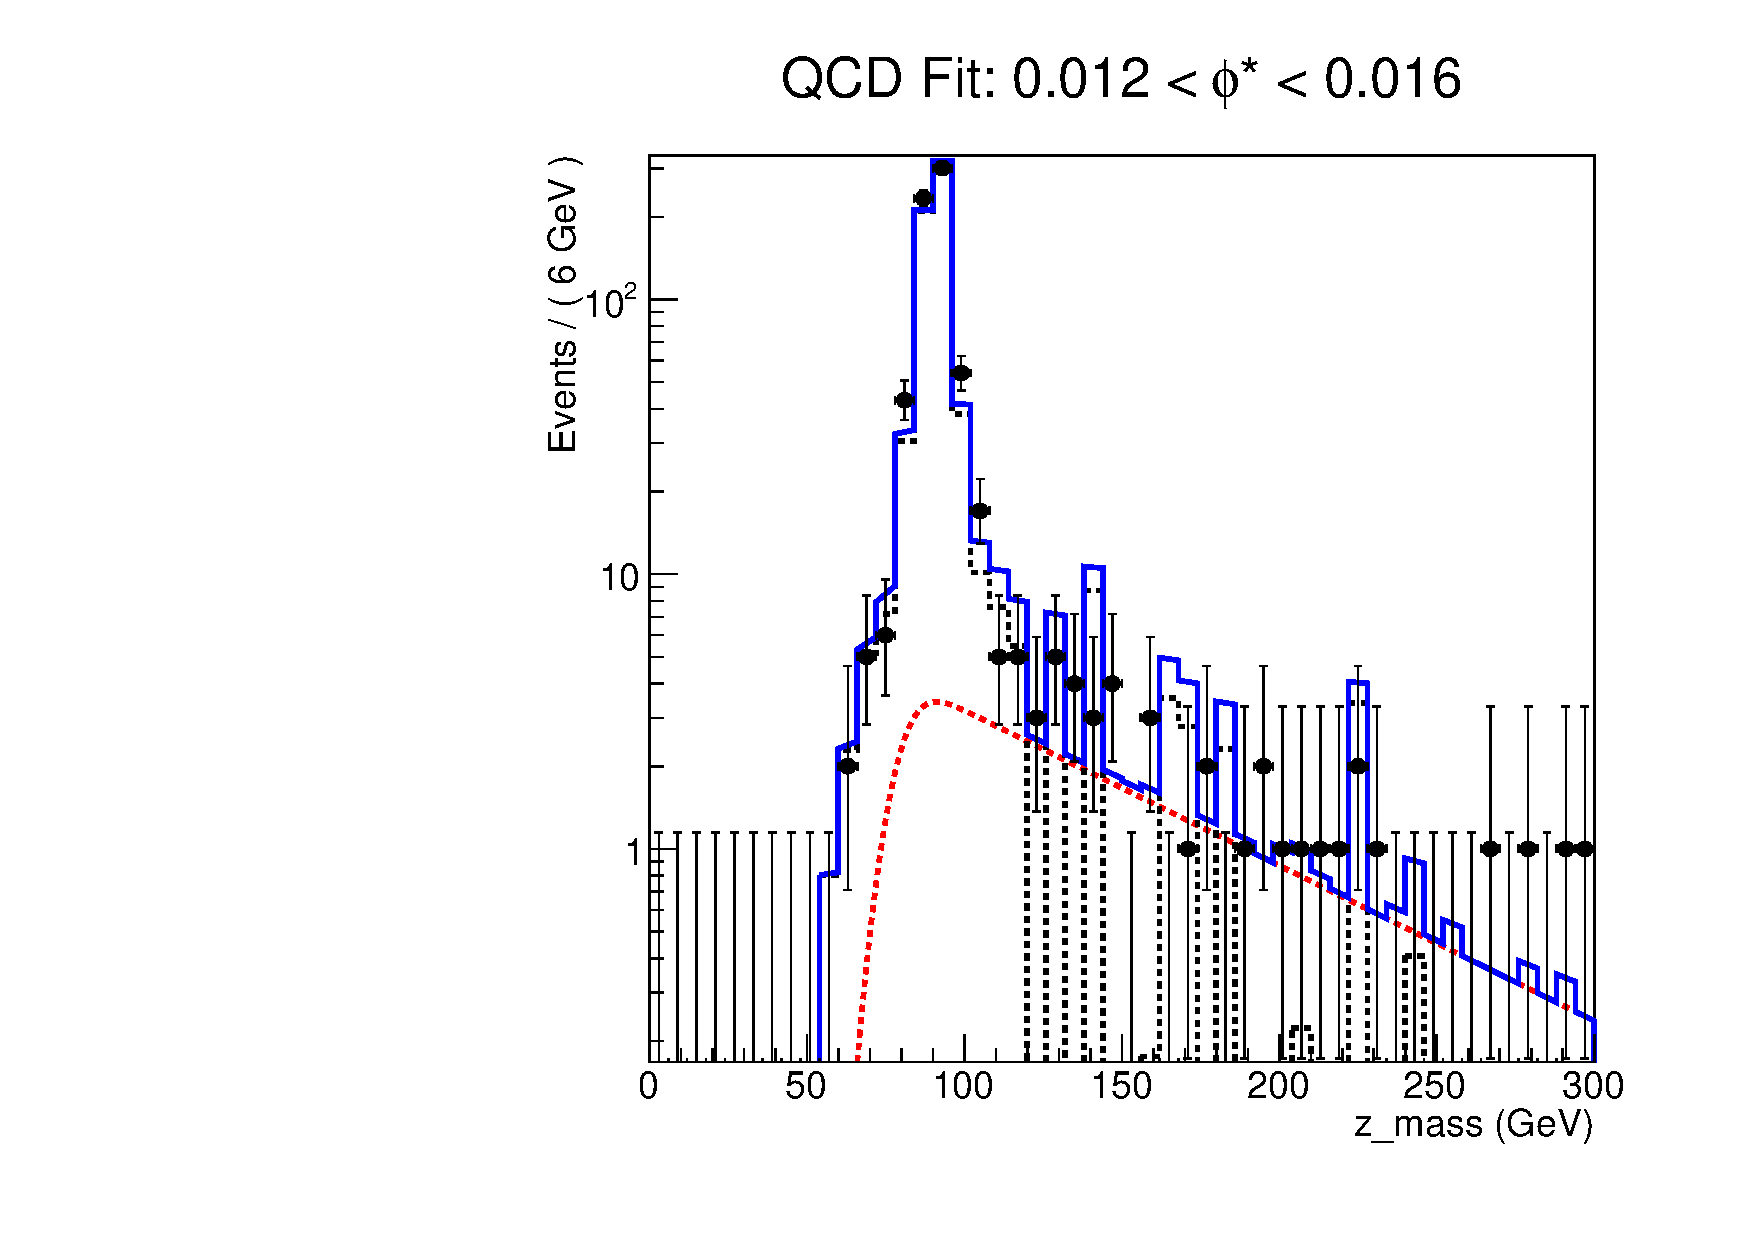
\includegraphics[width=\linewidth]{figures/qcd_fits/qcd_fit_plot_for_04.pdf}
        \label{fig:qcd_fit_04}
    \end{subfigure}
    \caption[
       The \QCDjets and \wjets data-driven background fits for the first set of
       four \phistar bins.
    ]{
       The \QCDjets and \wjets data-driven background fits for the first set of
       four \phistar bins. The data are shown as points with error bars, MC
       template as a dashed histogram, the analytic background function as the
       dashed line, and the sum of the template and function as a solid
       histogram.
    }
    \label{fig:qcd_many_1}
\end{figure}

\begin{figure}[!htbp]
    \centering
    \begin{subfigure}[b]{\SideBySidePlotWidth}
        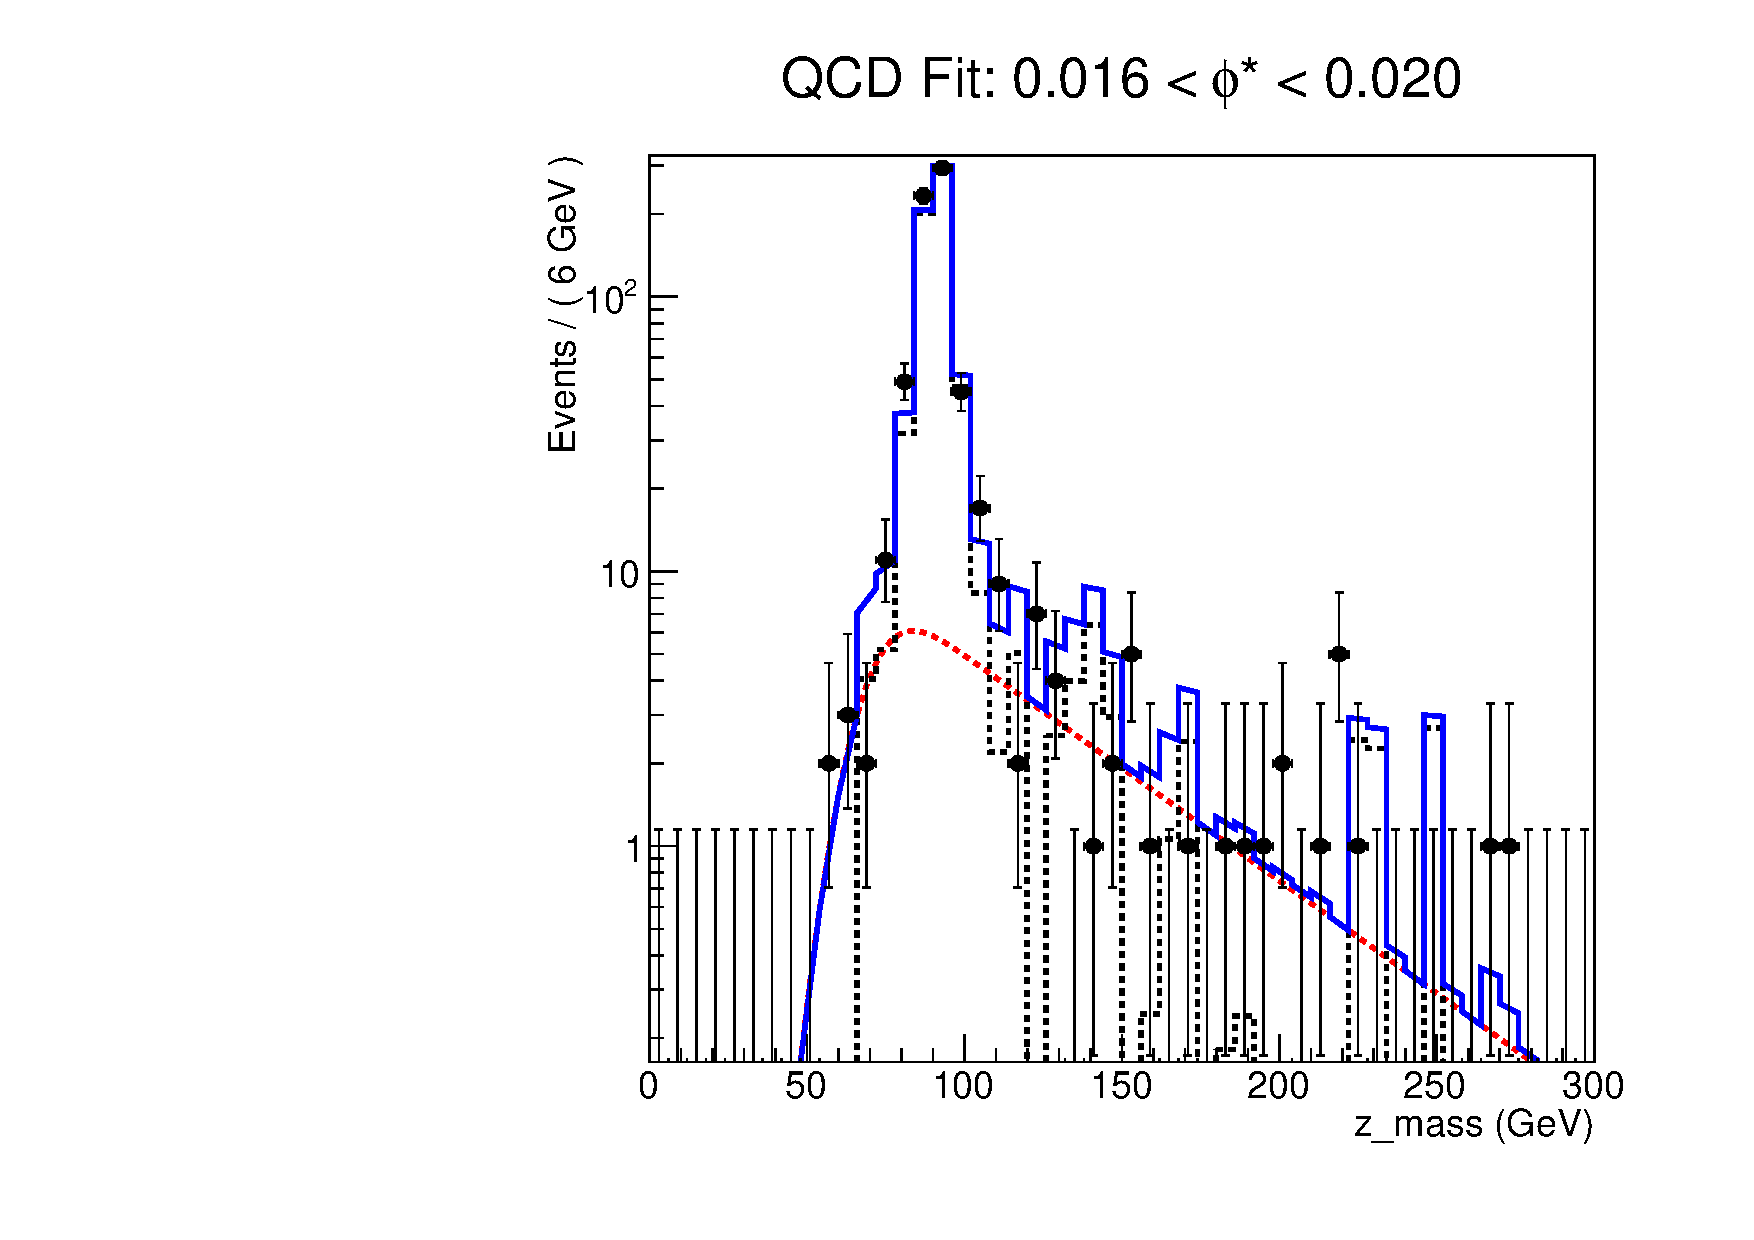
\includegraphics[width=\linewidth]{figures/qcd_fits/qcd_fit_plot_for_05.pdf}
        \label{fig:qcd_fit_05}
    \end{subfigure}%
    % The comment right after suppresses white space that would push the images
    % to new lines
    \begin{subfigure}[b]{\SideBySidePlotWidth}
        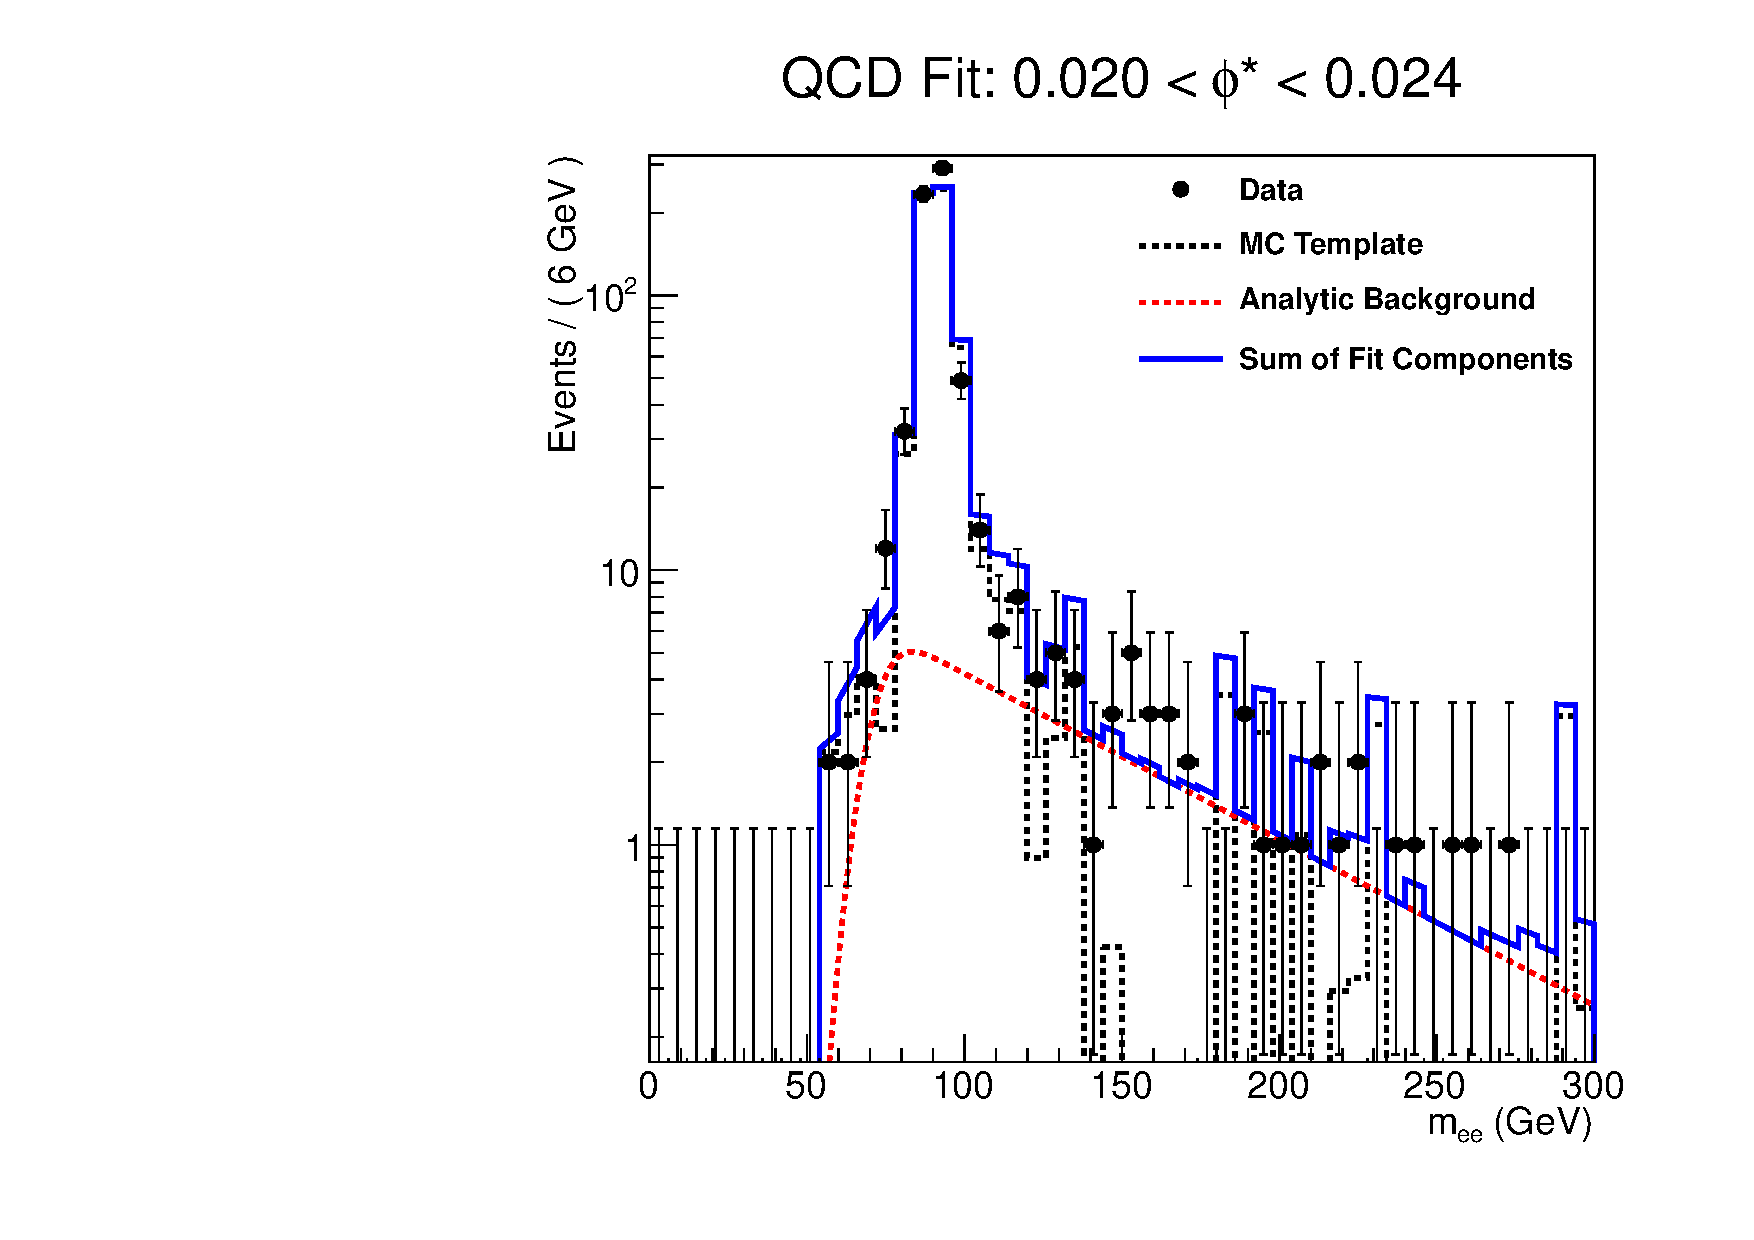
\includegraphics[width=\linewidth]{figures/qcd_fits/qcd_fit_plot_for_06.pdf}
        \label{fig:qcd_fit_06}
    \end{subfigure}
    % New line
    \begin{subfigure}[b]{\SideBySidePlotWidth}
        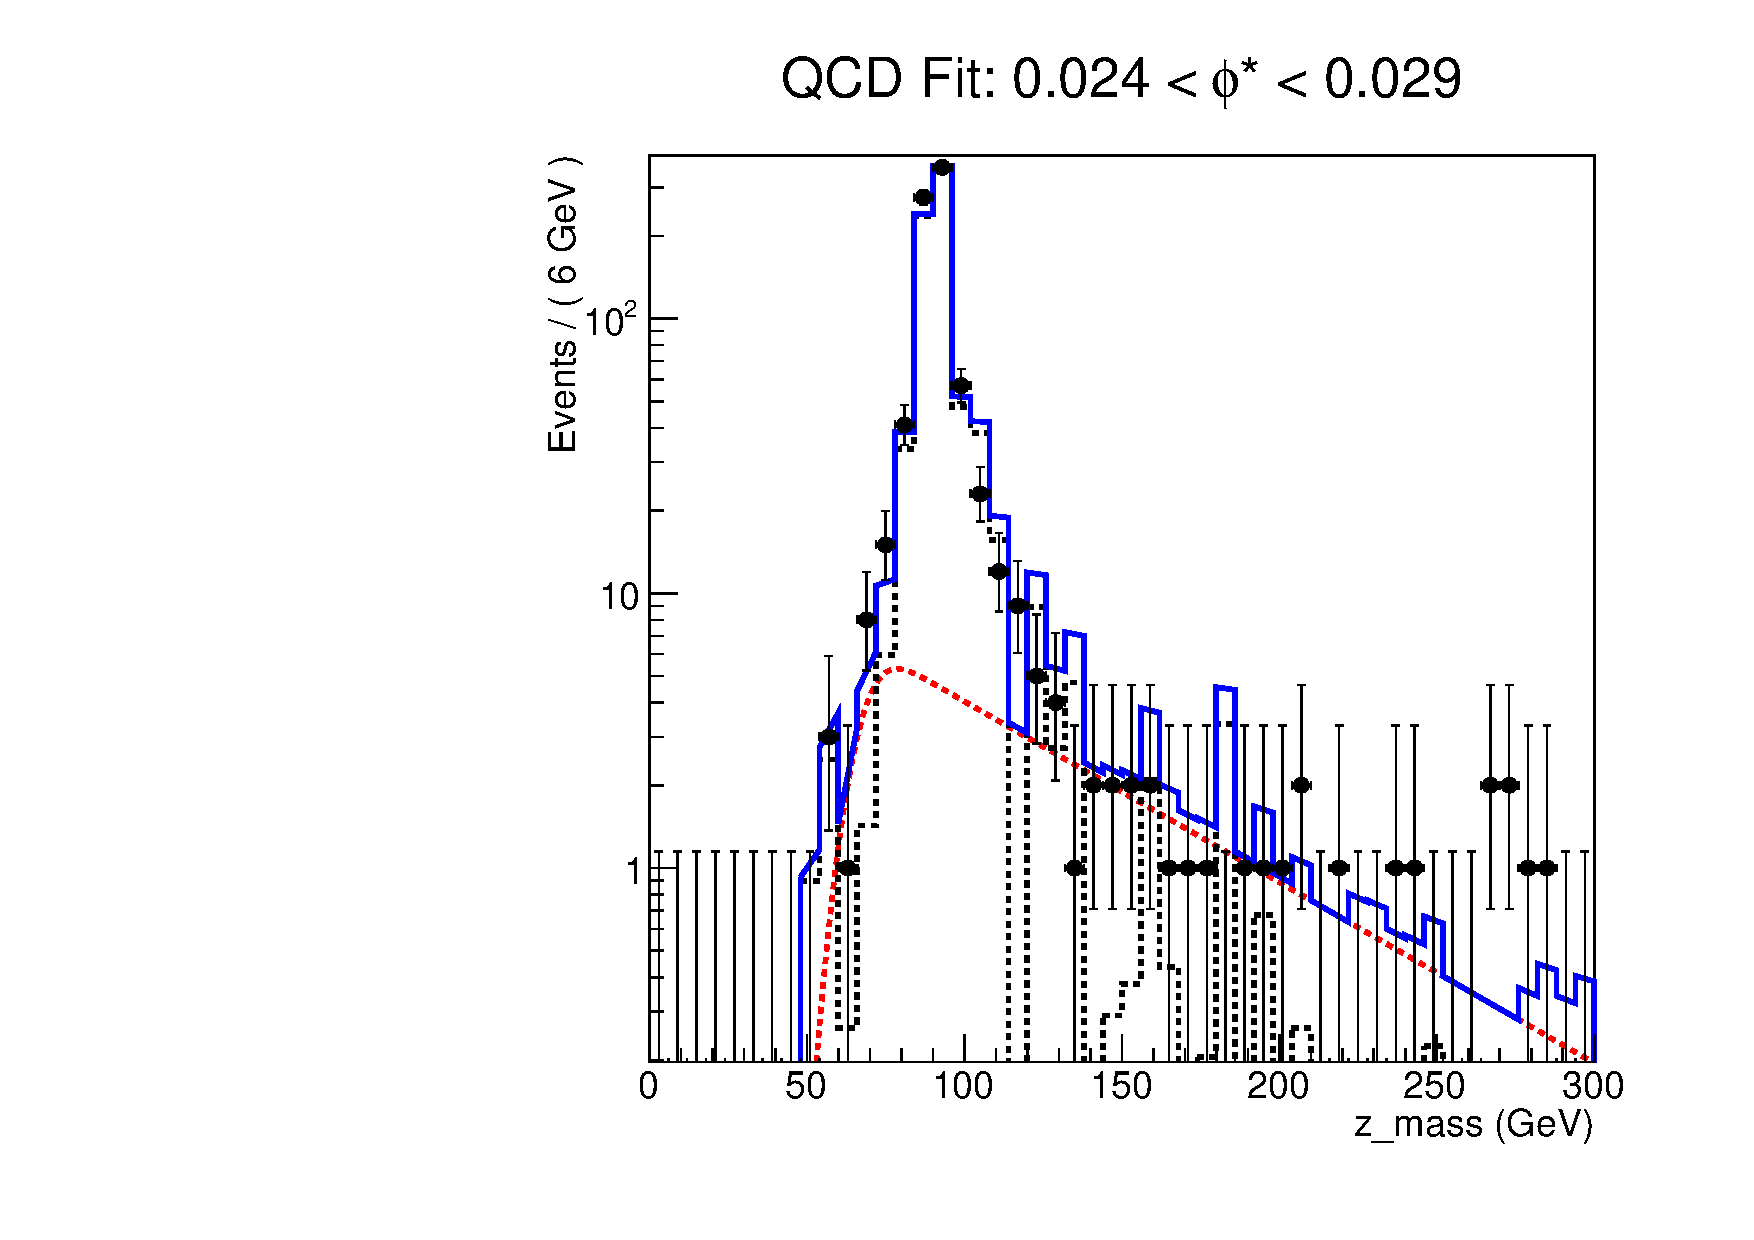
\includegraphics[width=\linewidth]{figures/qcd_fits/qcd_fit_plot_for_07.pdf}
        \label{fig:qcd_fit_07}
    \end{subfigure}%
    \begin{subfigure}[b]{\SideBySidePlotWidth}
        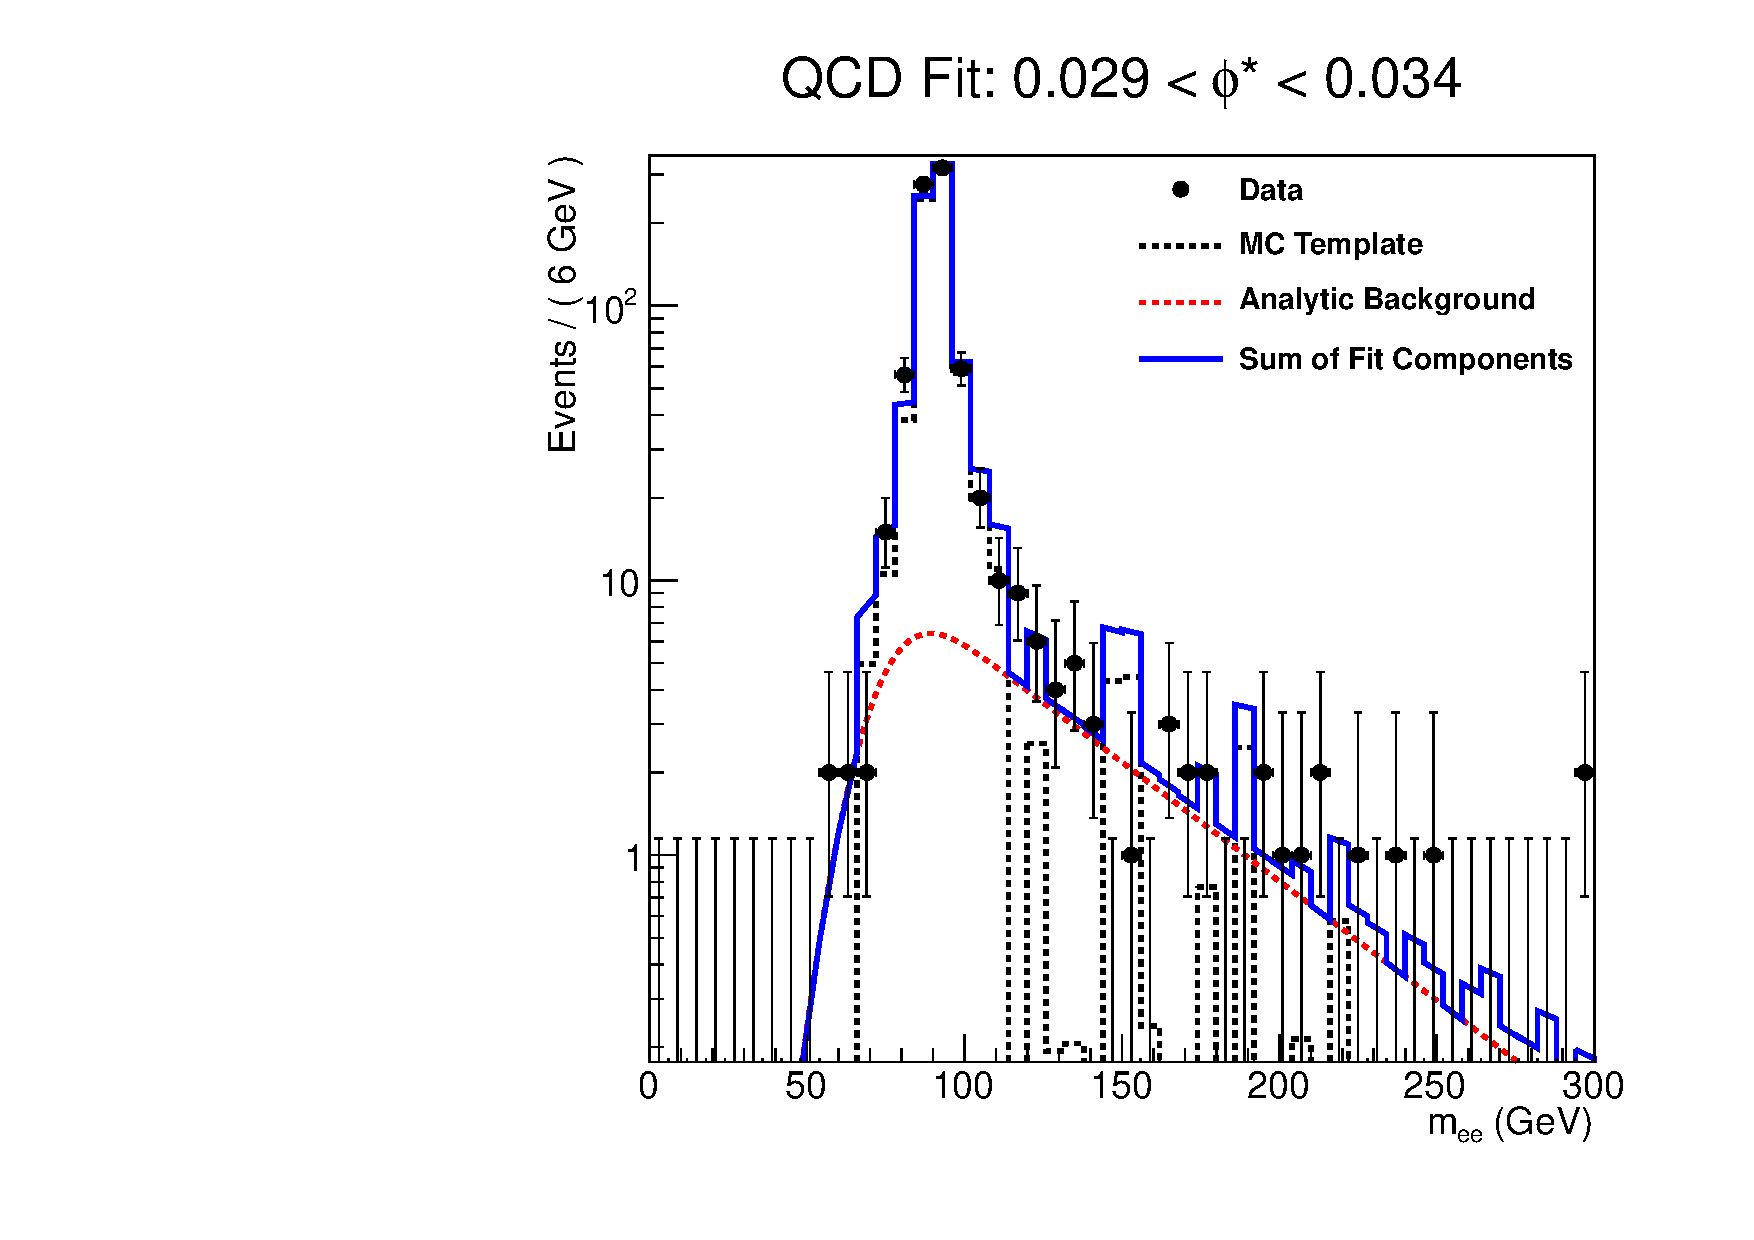
\includegraphics[width=\linewidth]{figures/qcd_fits/qcd_fit_plot_for_08.pdf}
        \label{fig:qcd_fit_08}
    \end{subfigure}
    \caption[
       The \QCDjets and \wjets data-driven background fits for the second set
       of four \phistar bins.
    ]{
       The \QCDjets and \wjets data-driven background fits for the second set
       of four \phistar bins. The data are shown as points with error bars, MC
       template as a dashed histogram, the analytic background function as the
       dashed line, and the sum of the template and function as a solid
       histogram.
    }
    \label{fig:qcd_many_2}
\end{figure}


\begin{figure}[!htbp]
    \centering
    \begin{subfigure}[b]{\SideBySidePlotWidth}
        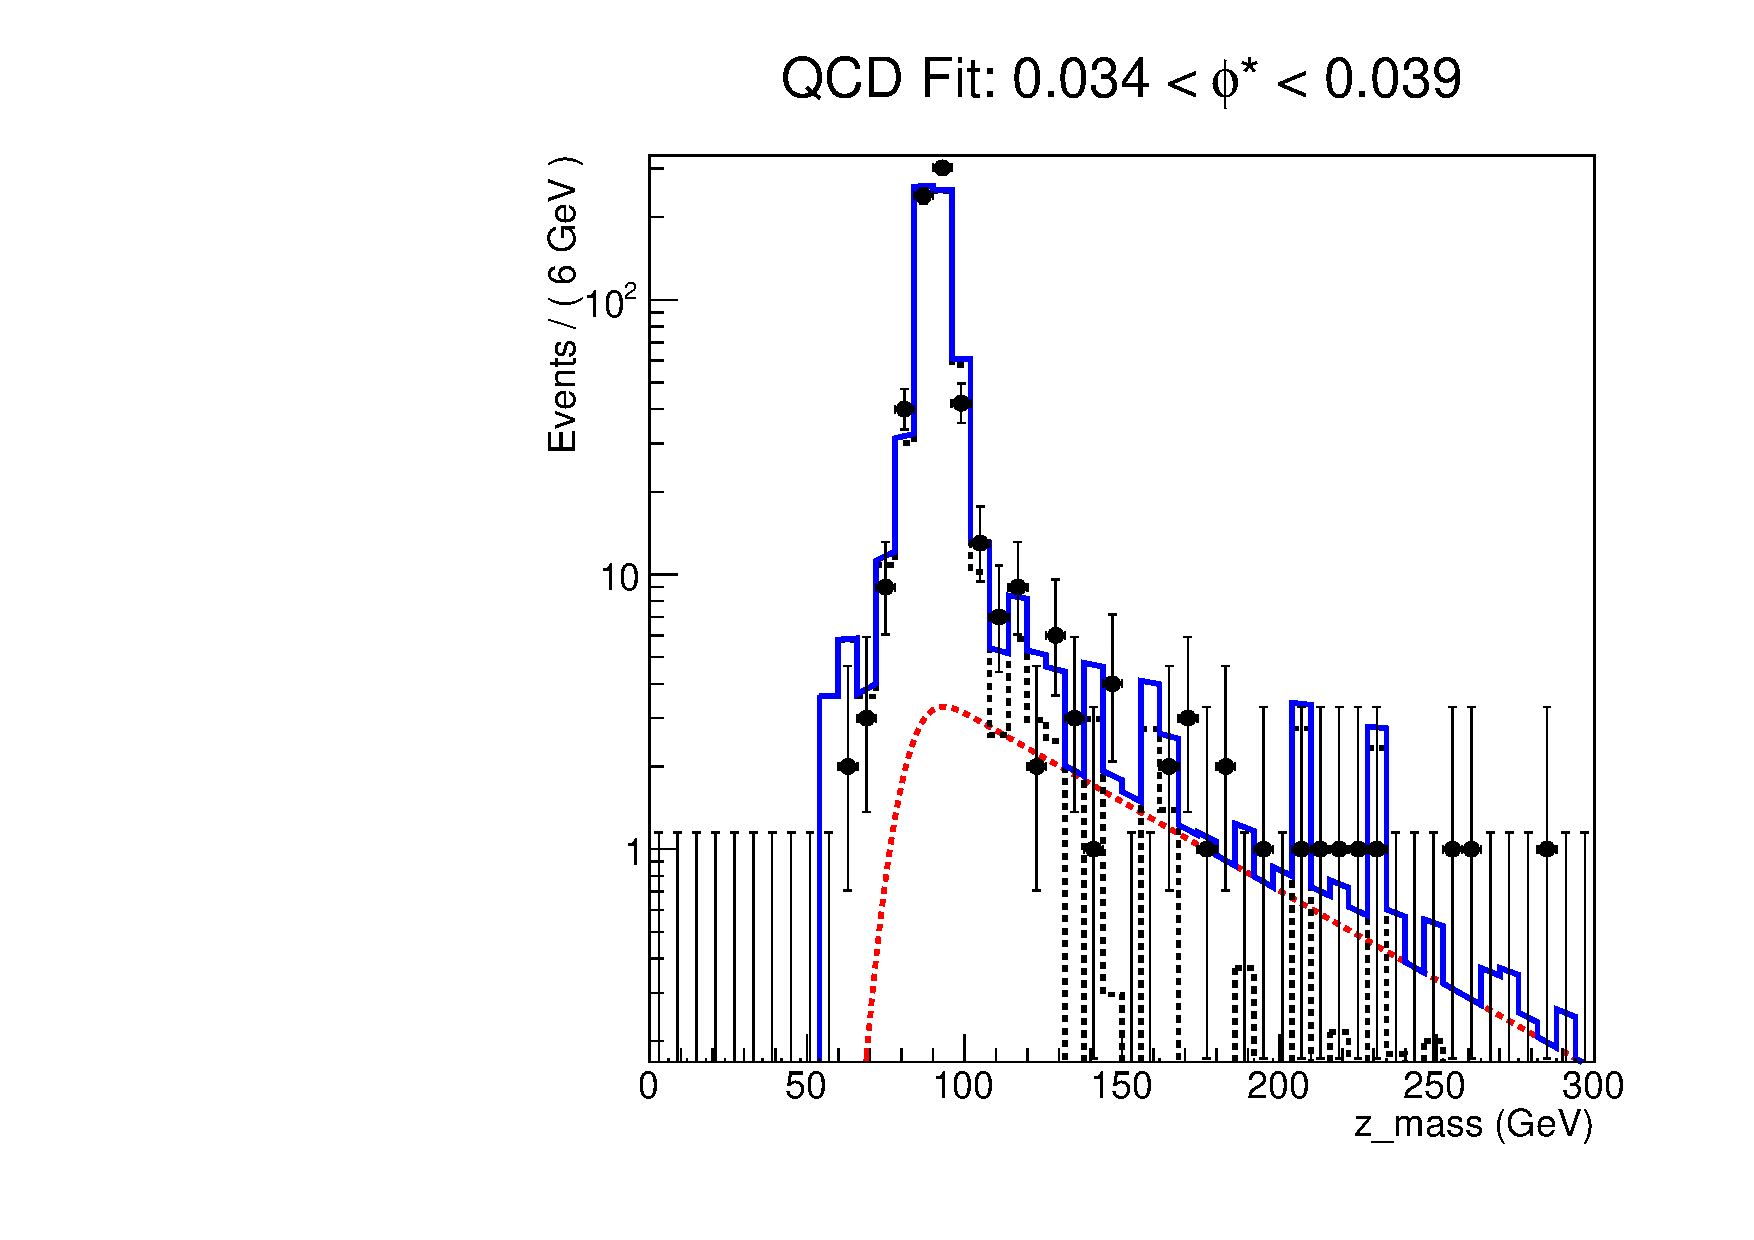
\includegraphics[width=\linewidth]{figures/qcd_fits/qcd_fit_plot_for_09.pdf}
        \label{fig:qcd_fit_09}
    \end{subfigure}%
    % The comment right after suppresses white space that would push the images
    % to new lines
    \begin{subfigure}[b]{\SideBySidePlotWidth}
        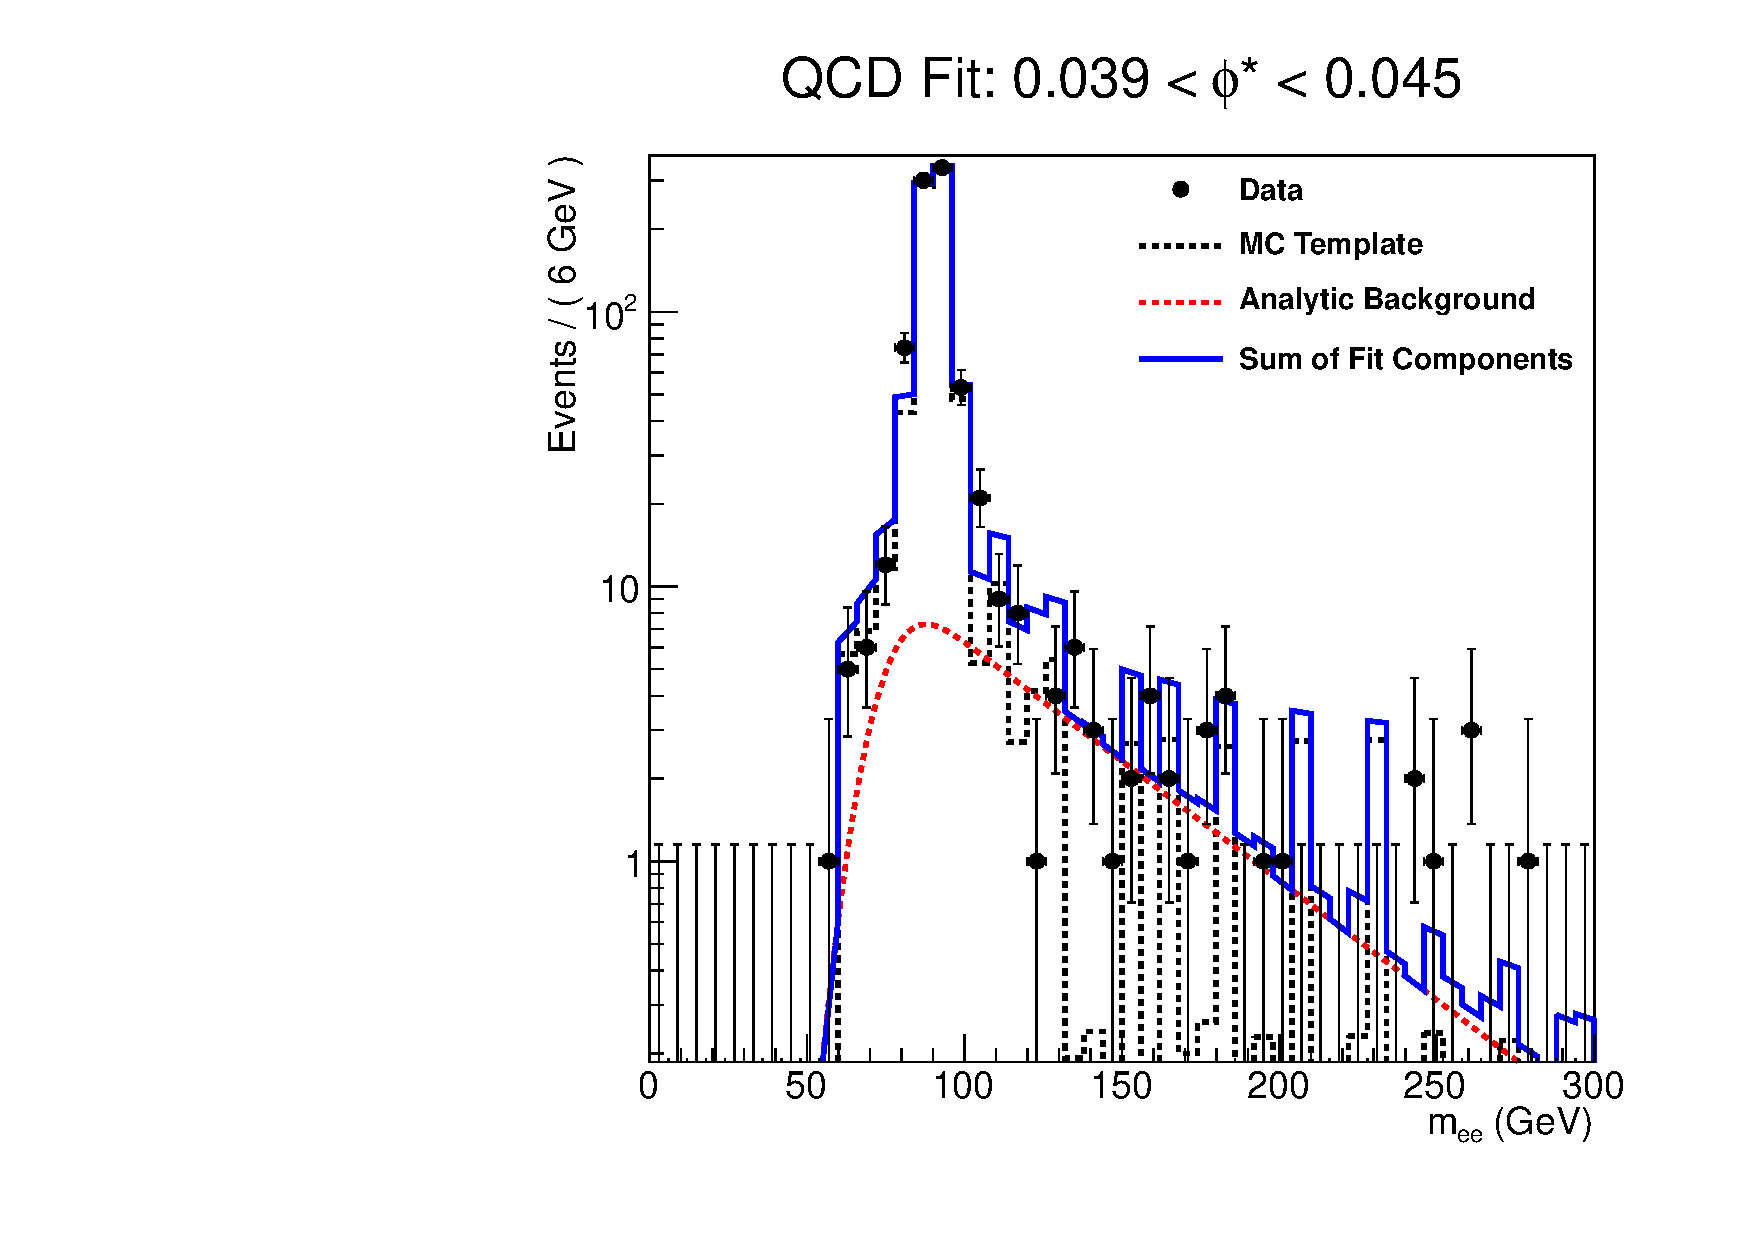
\includegraphics[width=\linewidth]{figures/qcd_fits/qcd_fit_plot_for_10.pdf}
        \label{fig:qcd_fit_10}
    \end{subfigure}
    % New line
    \begin{subfigure}[b]{\SideBySidePlotWidth}
        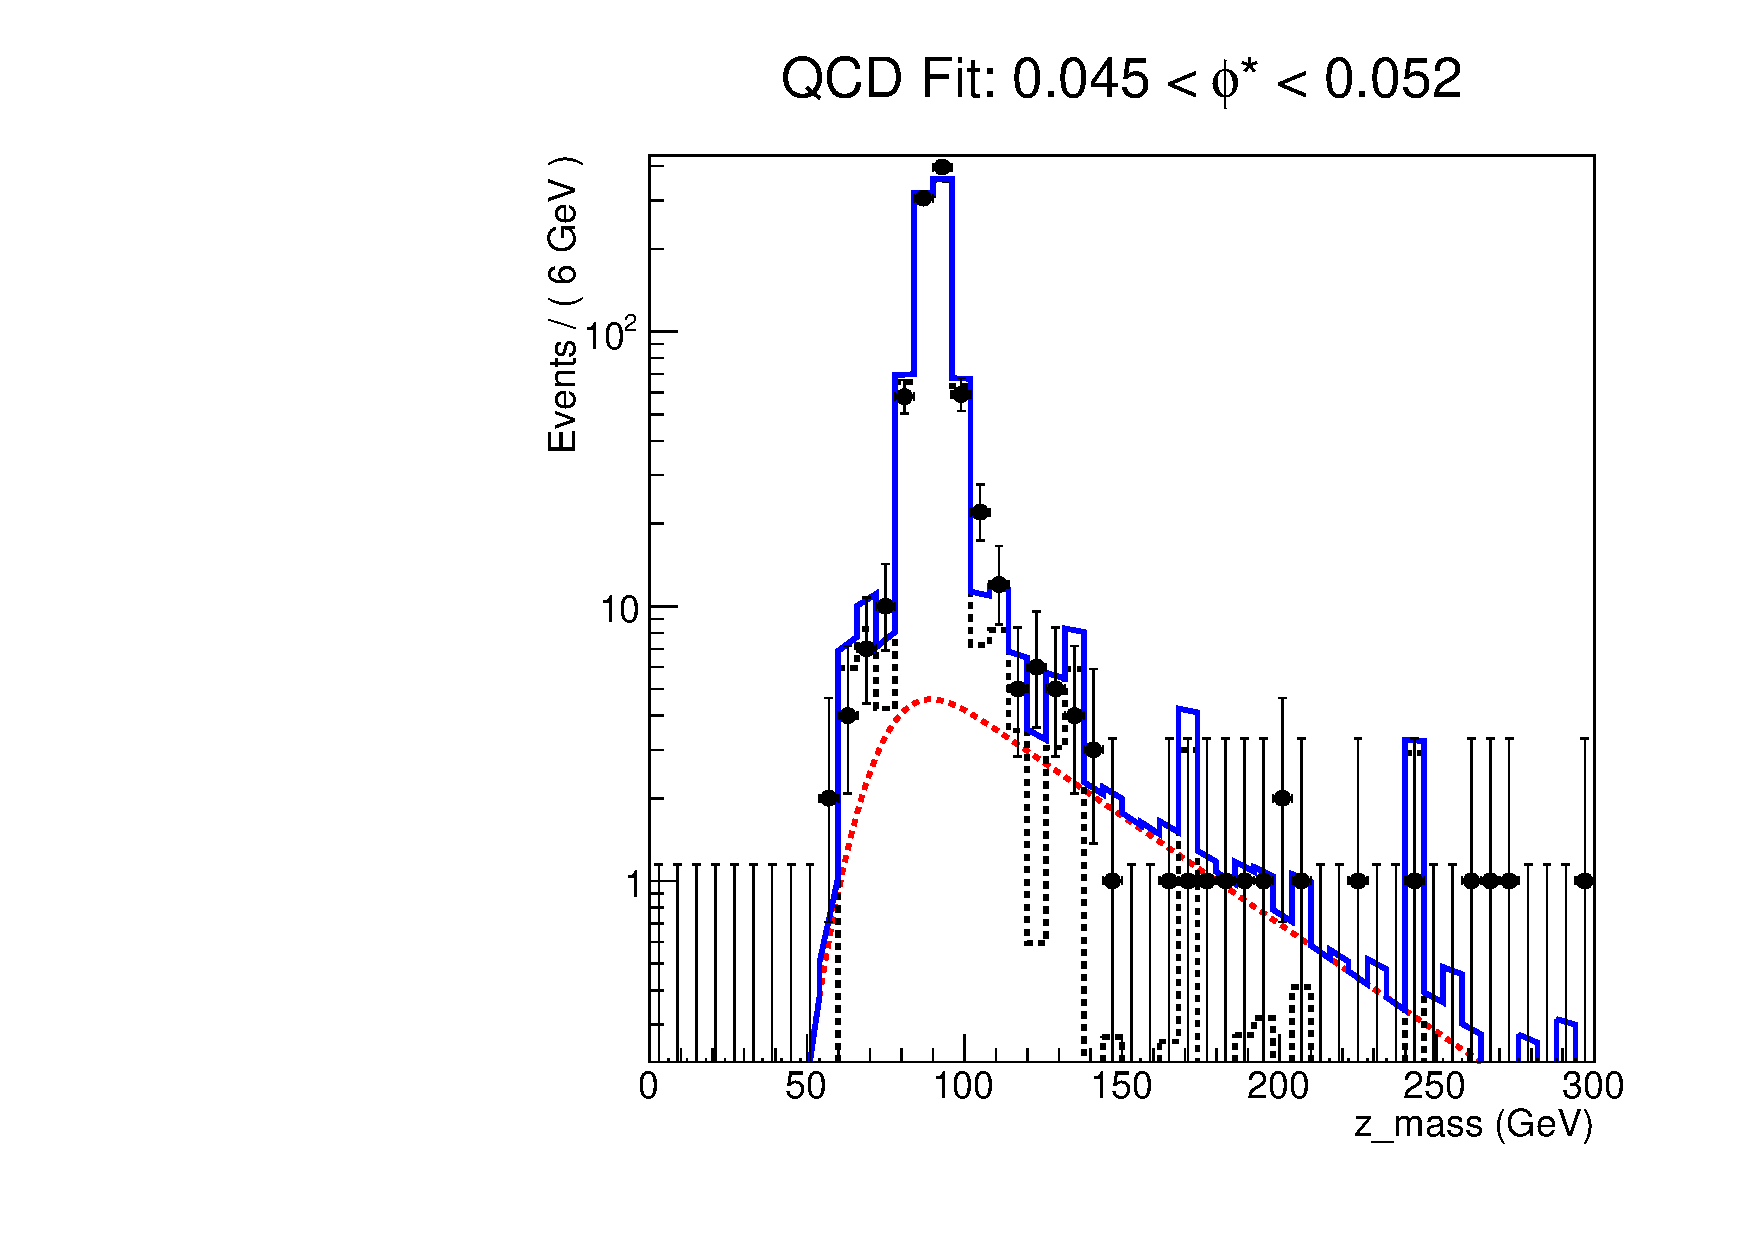
\includegraphics[width=\linewidth]{figures/qcd_fits/qcd_fit_plot_for_11.pdf}
        \label{fig:qcd_fit_11}
    \end{subfigure}%
    \begin{subfigure}[b]{\SideBySidePlotWidth}
        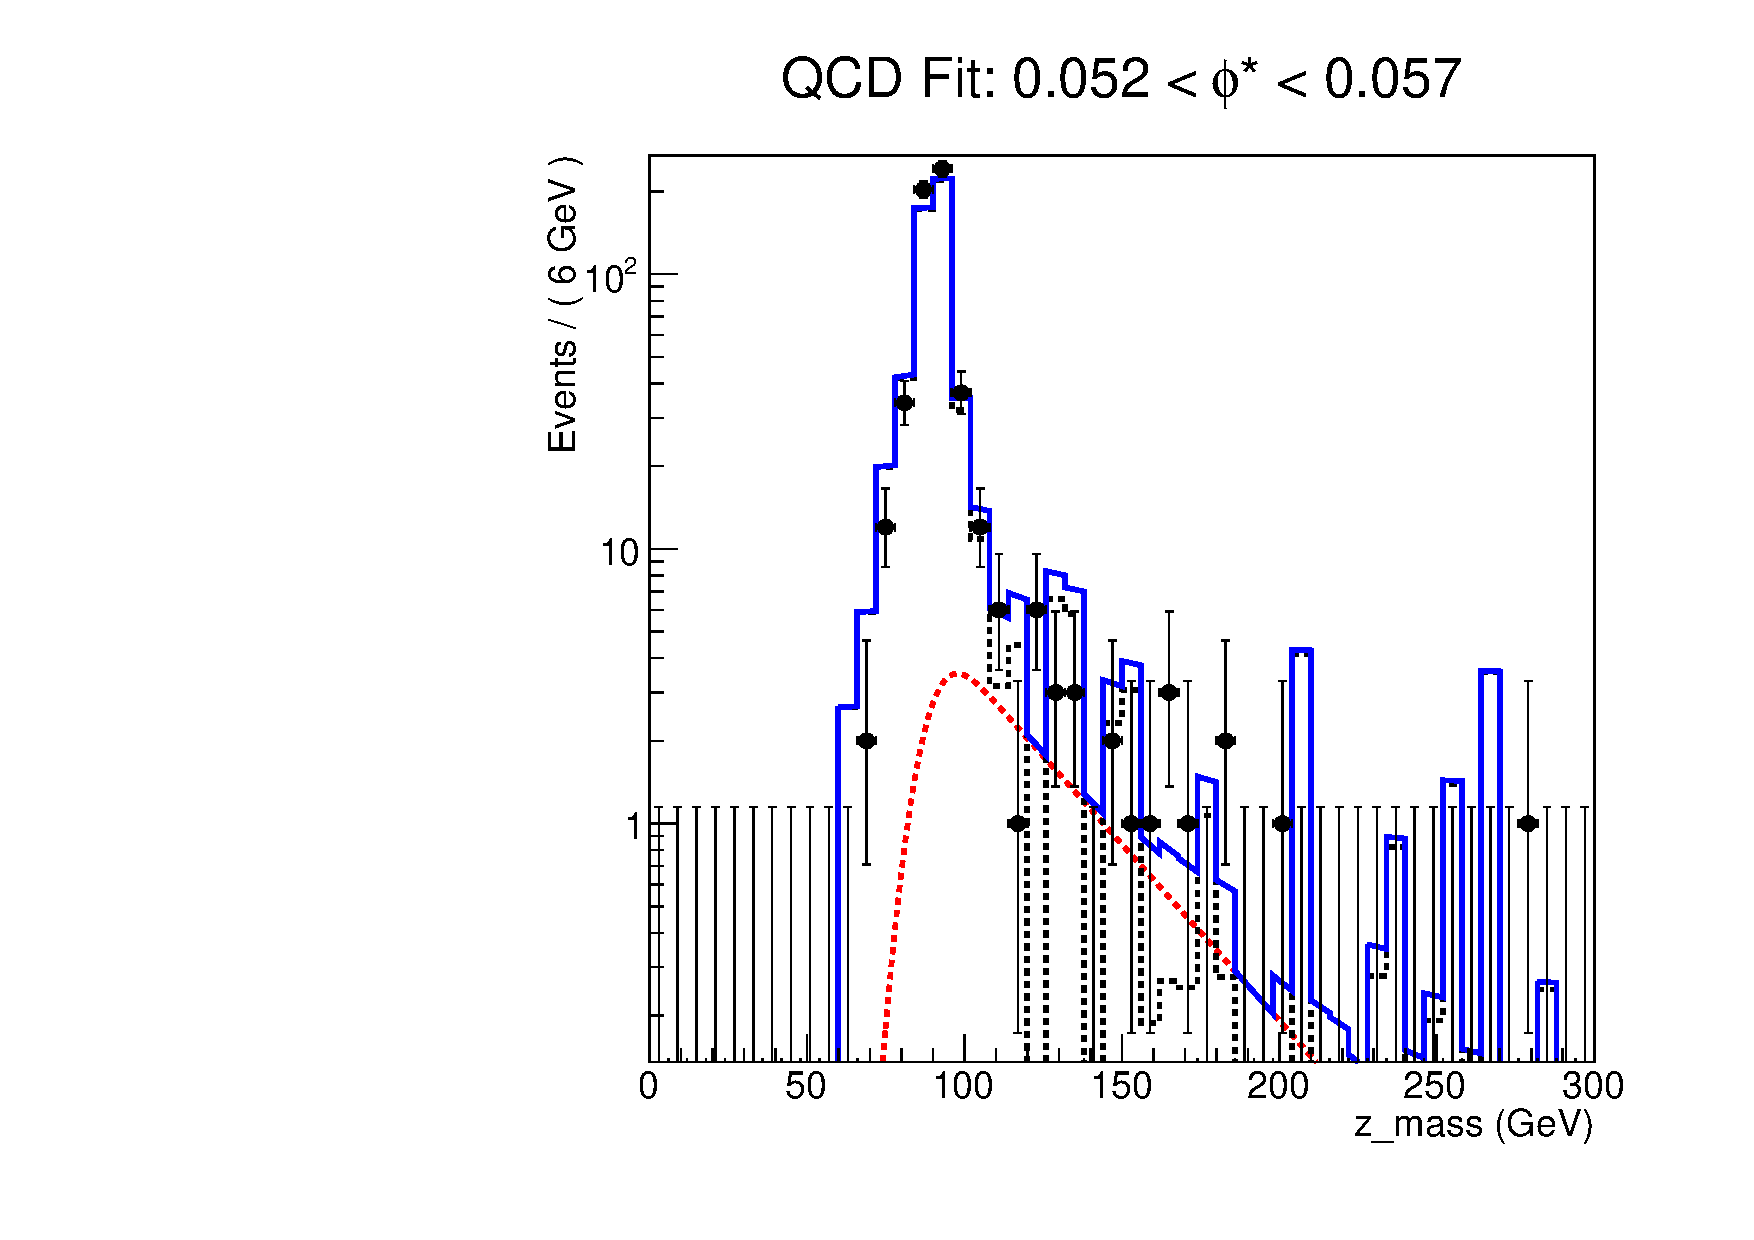
\includegraphics[width=\linewidth]{figures/qcd_fits/qcd_fit_plot_for_12.pdf}
        \label{fig:qcd_fit_12}
    \end{subfigure}
    \caption[
       The \QCDjets and \wjets data-driven background fits for the third set of
       four \phistar bins.
    ]{
       The \QCDjets and \wjets data-driven background fits for the third set of
       four \phistar bins. The data are shown as points with error bars, MC
       template as a dashed histogram, the analytic background function as the
       dashed line, and the sum of the template and function as a solid
       histogram.
    }
    \label{fig:qcd_many_3}
\end{figure}


\begin{figure}[!htbp]
    \centering
    \begin{subfigure}[b]{\SideBySidePlotWidth}
        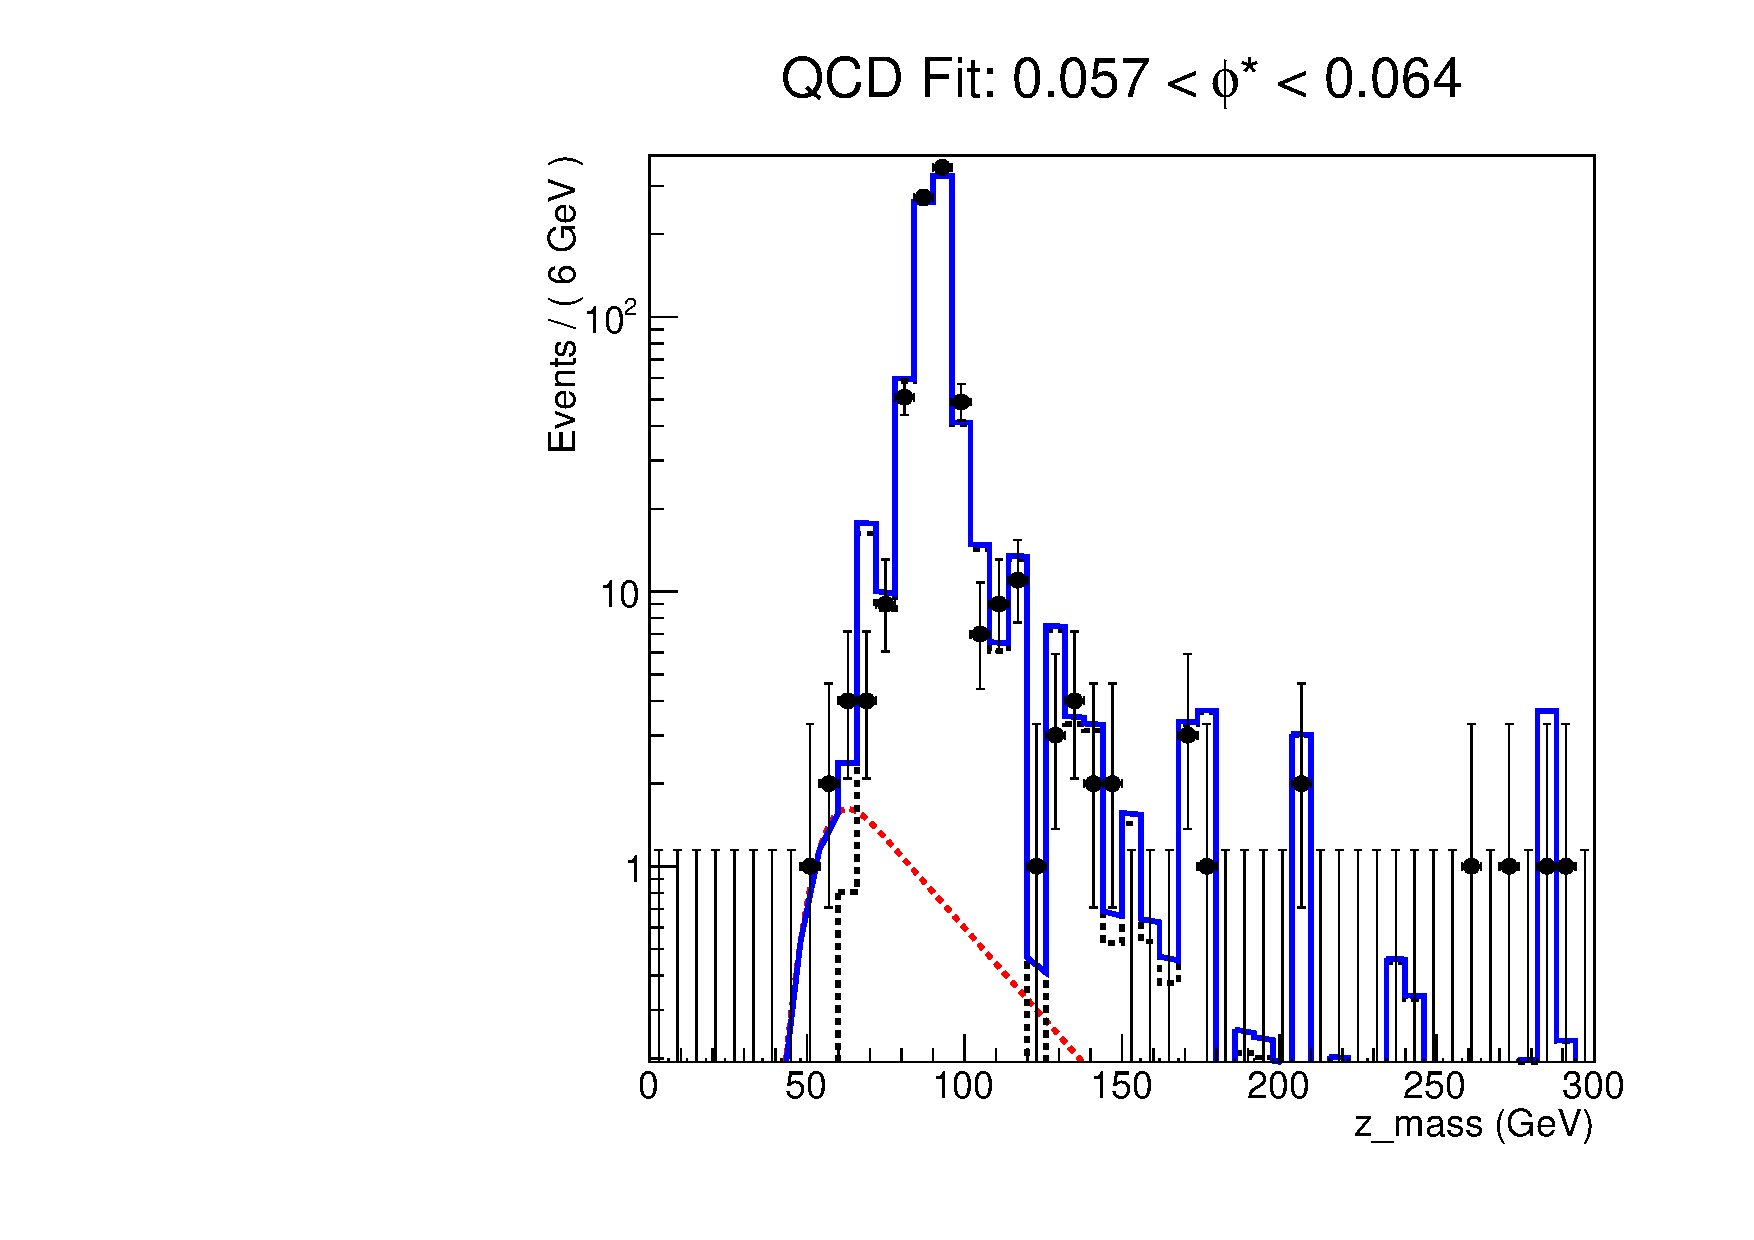
\includegraphics[width=\linewidth]{figures/qcd_fits/qcd_fit_plot_for_13.pdf}
        \label{fig:qcd_fit_13}
    \end{subfigure}%
    % The comment right after suppresses white space that would push the images
    % to new lines
    \begin{subfigure}[b]{\SideBySidePlotWidth}
        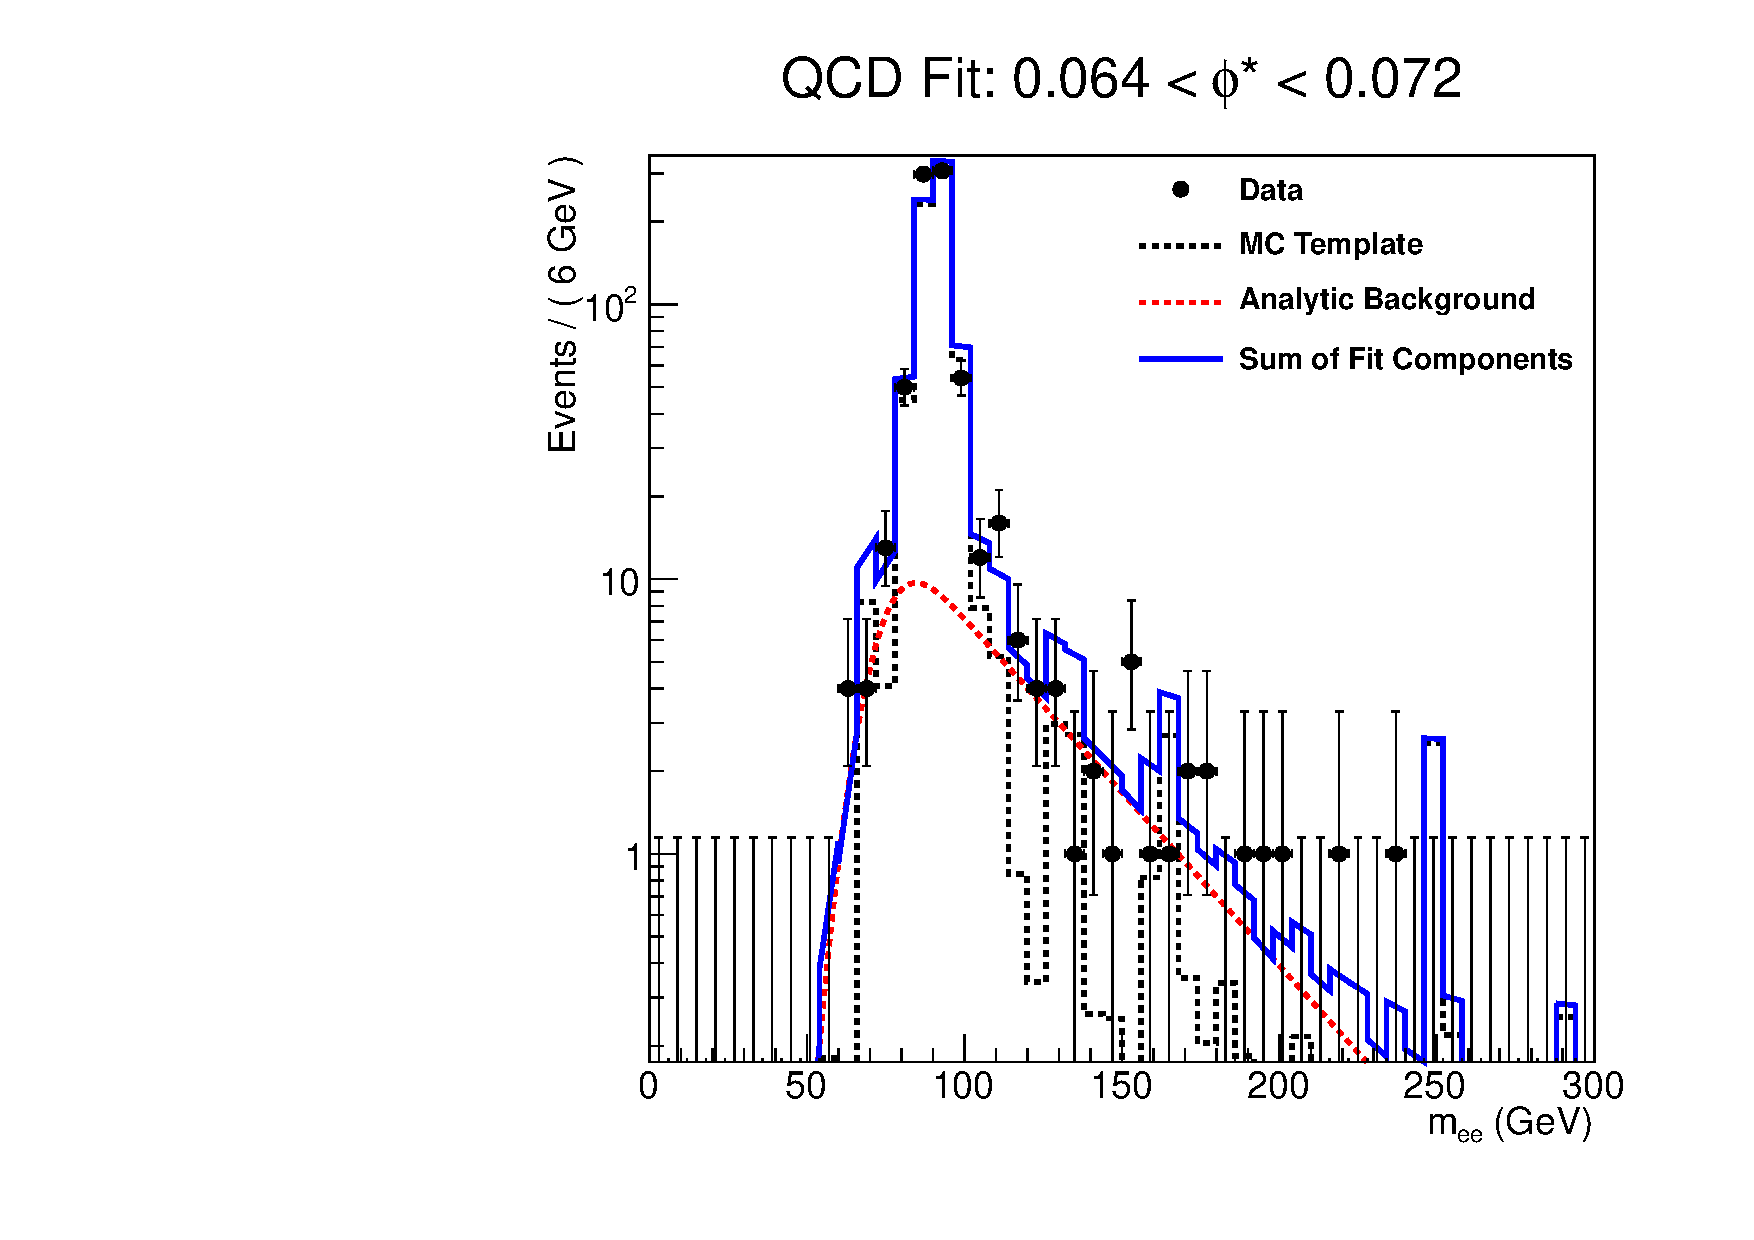
\includegraphics[width=\linewidth]{figures/qcd_fits/qcd_fit_plot_for_14.pdf}
        \label{fig:qcd_fit_14}
    \end{subfigure}
    % New line
    \begin{subfigure}[b]{\SideBySidePlotWidth}
        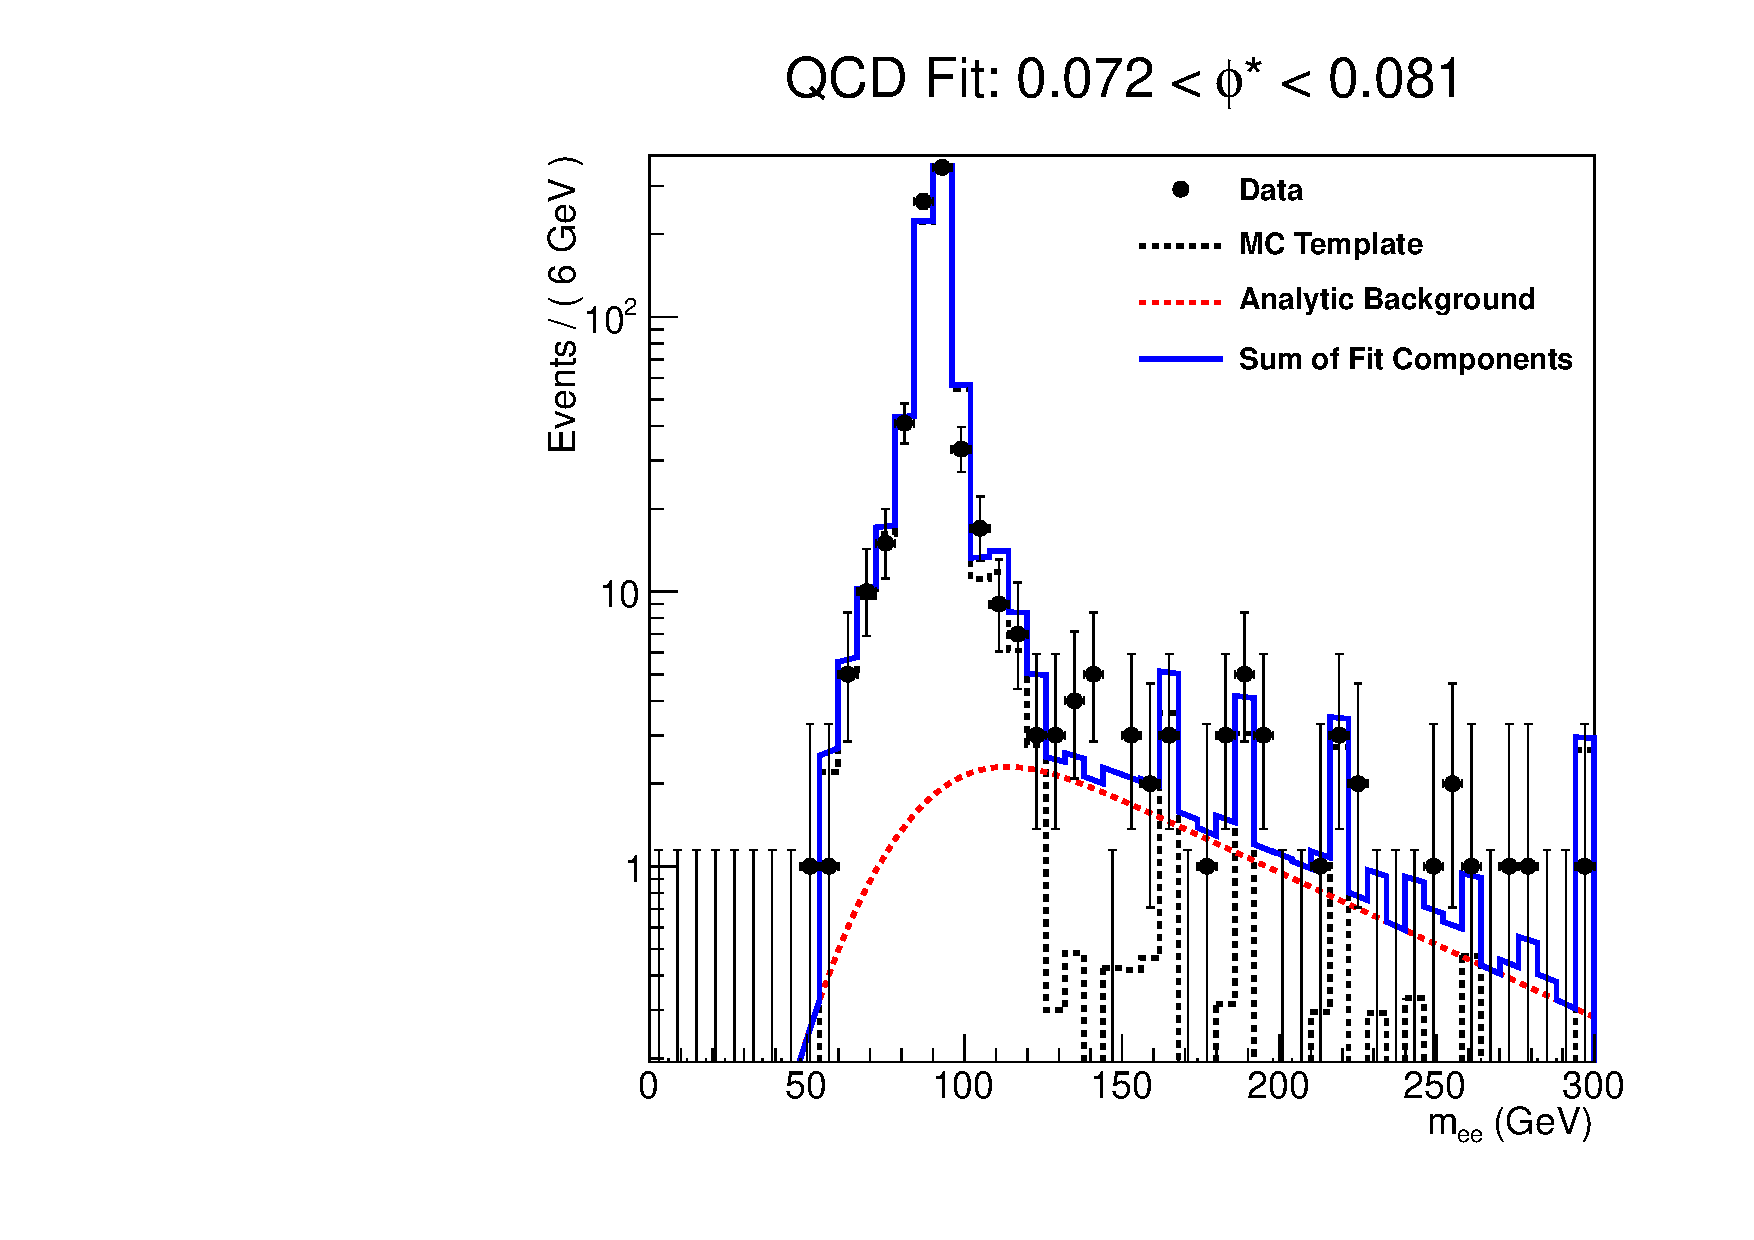
\includegraphics[width=\linewidth]{figures/qcd_fits/qcd_fit_plot_for_15.pdf}
        \label{fig:qcd_fit_15}
    \end{subfigure}%
    \begin{subfigure}[b]{\SideBySidePlotWidth}
        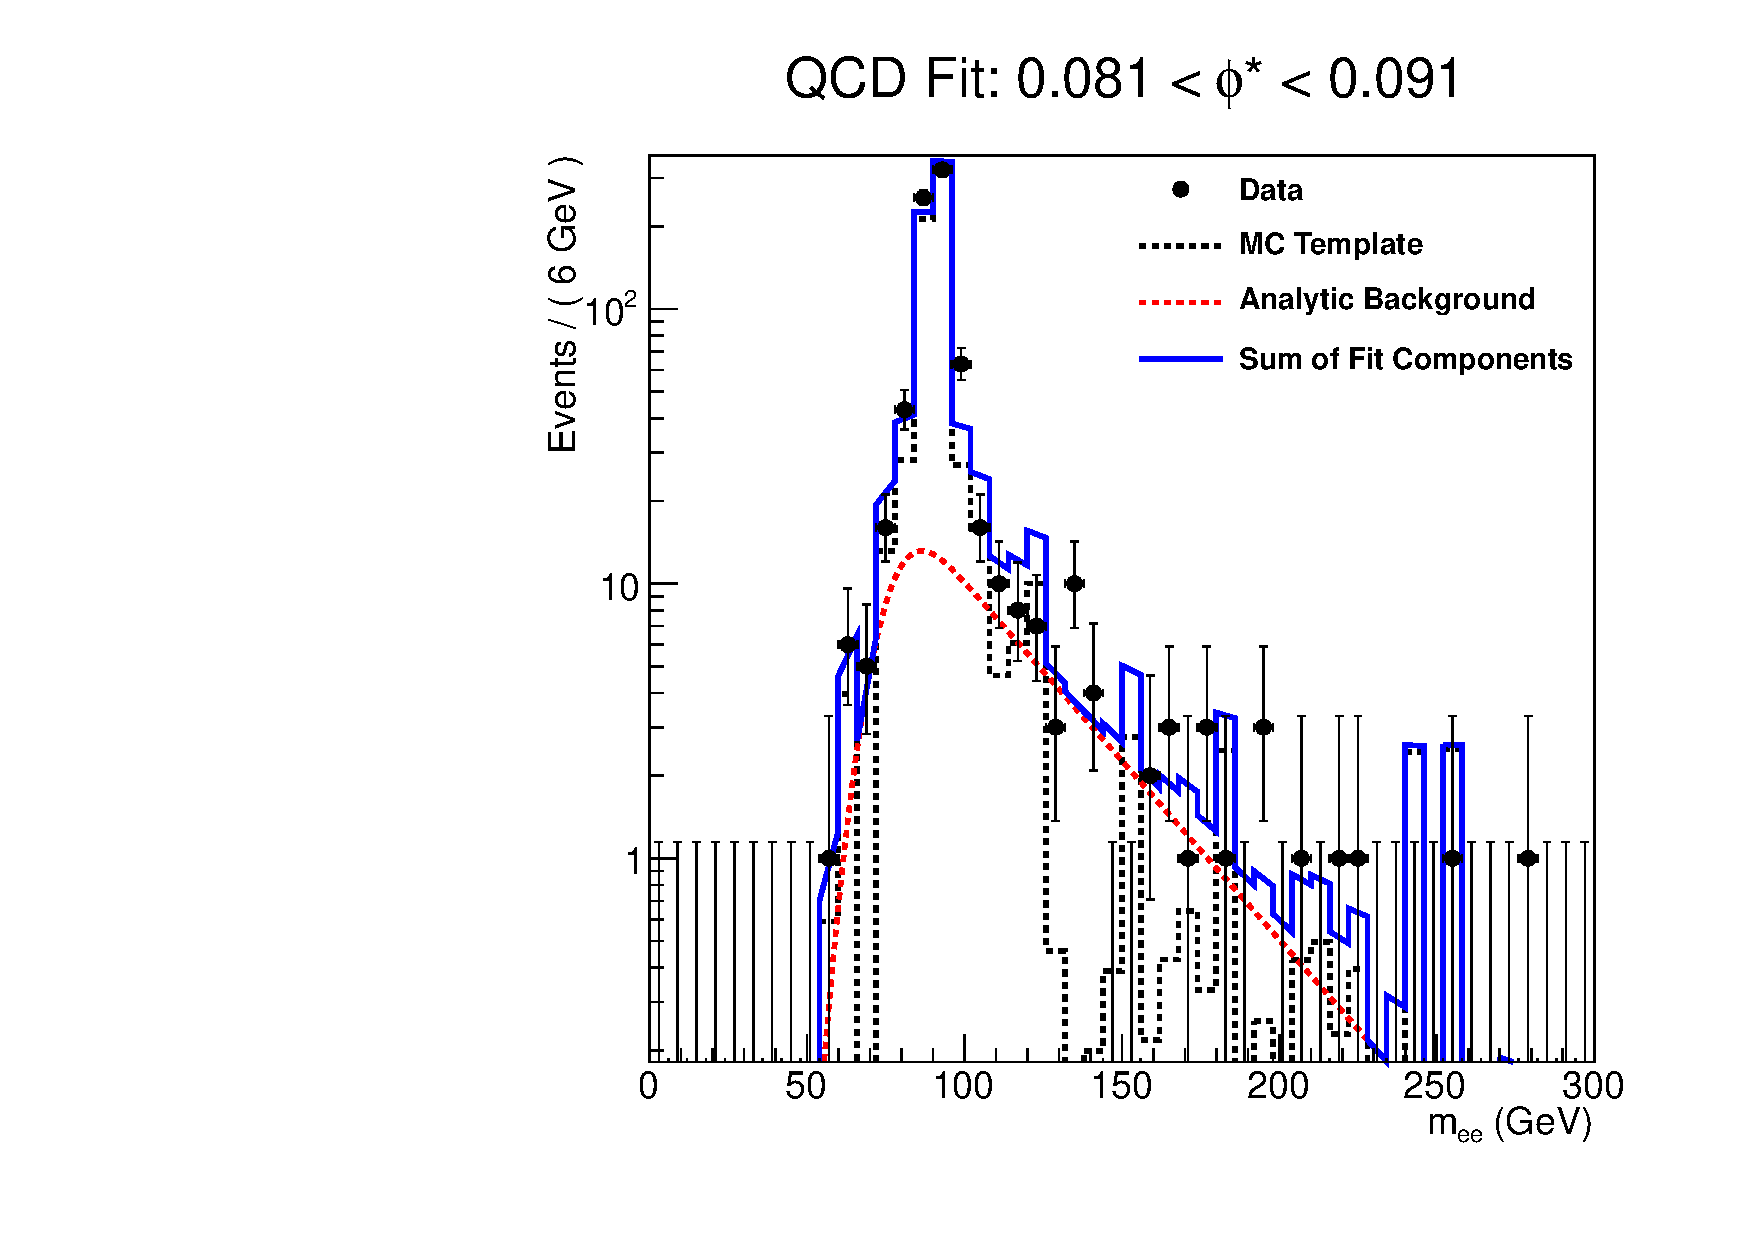
\includegraphics[width=\linewidth]{figures/qcd_fits/qcd_fit_plot_for_16.pdf}
        \label{fig:qcd_fit_16}
    \end{subfigure}
    \caption[
       The \QCDjets and \wjets data-driven background fits for the forth set of
       four \phistar bins.
    ]{
       The \QCDjets and \wjets data-driven background fits for the forth set of
       four \phistar bins. The data are shown as points with error bars, MC
       template as a dashed histogram, the analytic background function as the
       dashed line, and the sum of the template and function as a solid
       histogram.
    }
    \label{fig:qcd_many_4}
\end{figure}

\begin{figure}[!htbp]
    \centering
    \begin{subfigure}[b]{\SideBySidePlotWidth}
        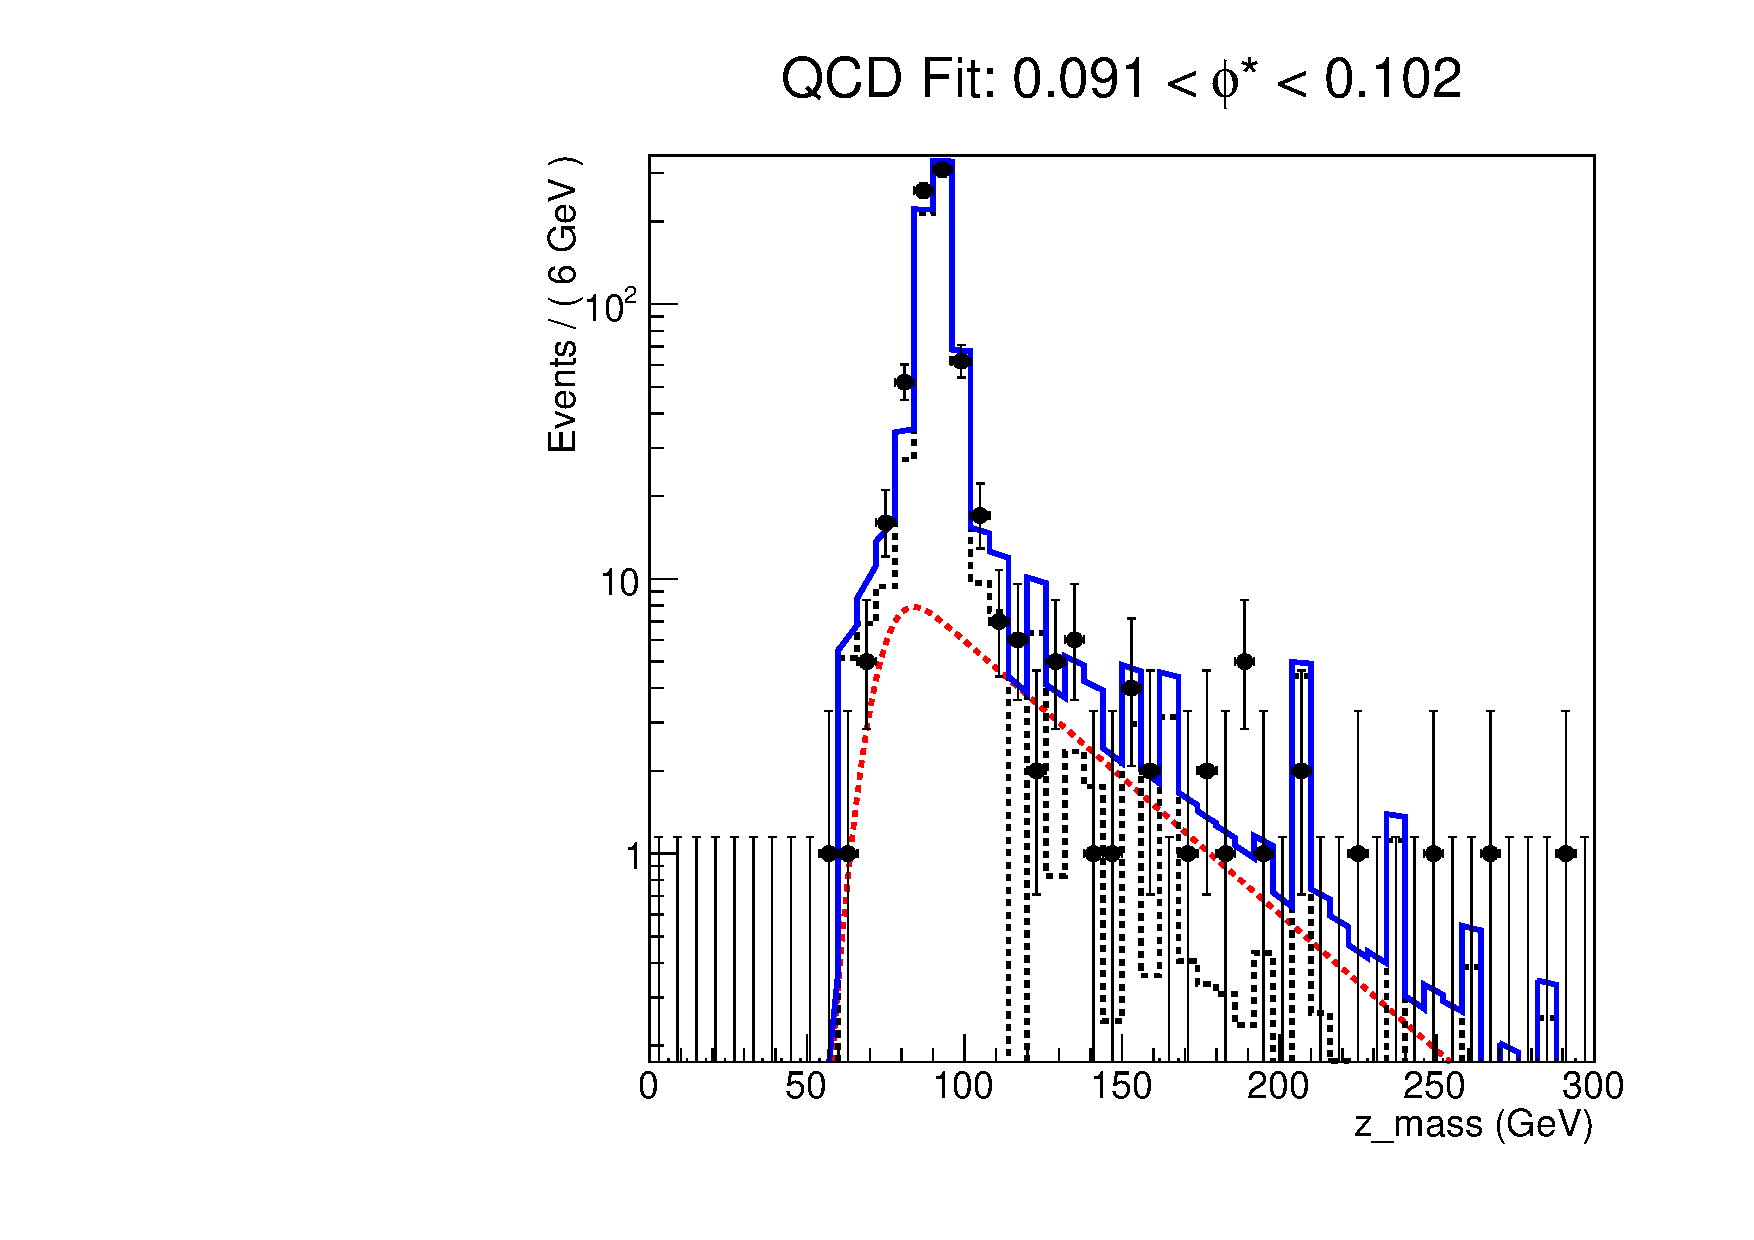
\includegraphics[width=\linewidth]{figures/qcd_fits/qcd_fit_plot_for_17.pdf}
        \label{fig:qcd_fit_17}
    \end{subfigure}%
    % The comment right after suppresses white space that would push the images
    % to new lines
    \begin{subfigure}[b]{\SideBySidePlotWidth}
        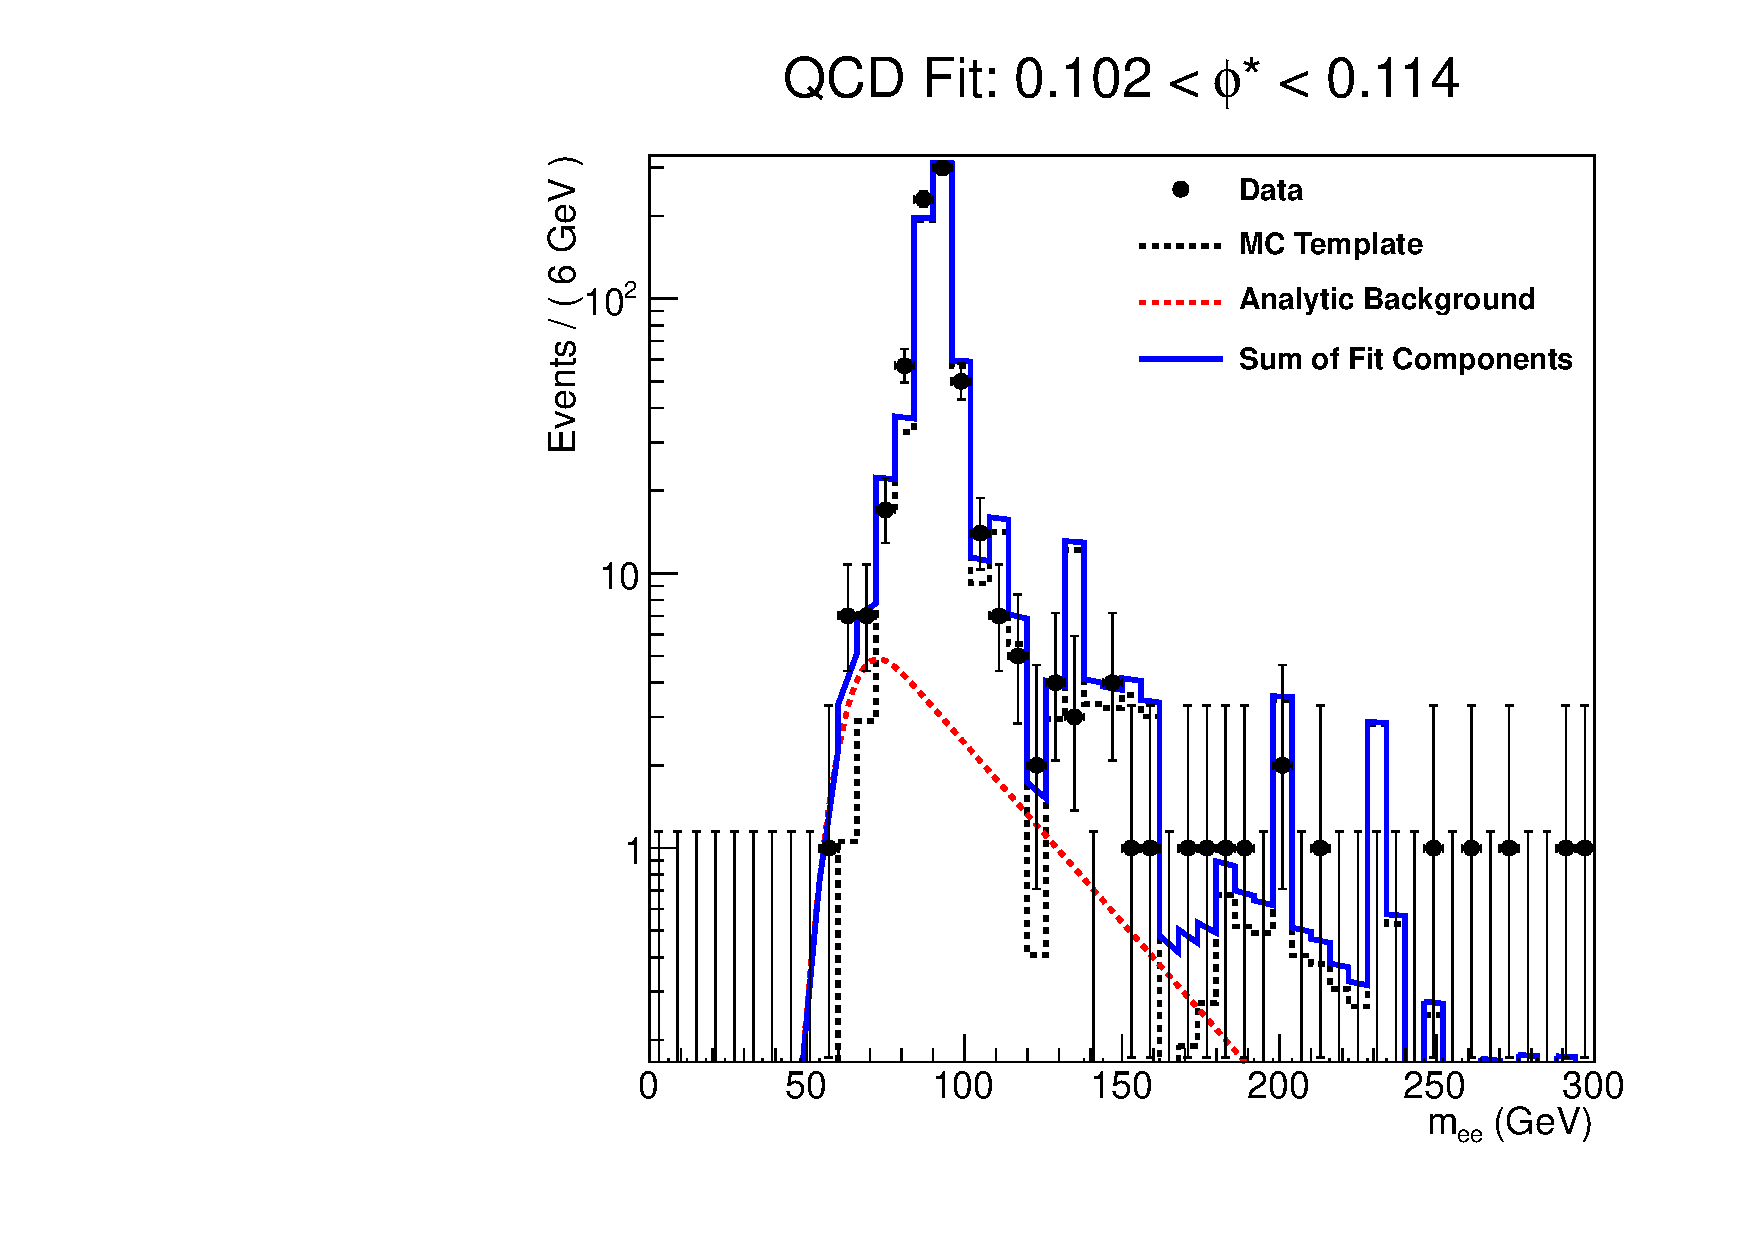
\includegraphics[width=\linewidth]{figures/qcd_fits/qcd_fit_plot_for_18.pdf}
        \label{fig:qcd_fit_18}
    \end{subfigure}
    % New line
    \begin{subfigure}[b]{\SideBySidePlotWidth}
        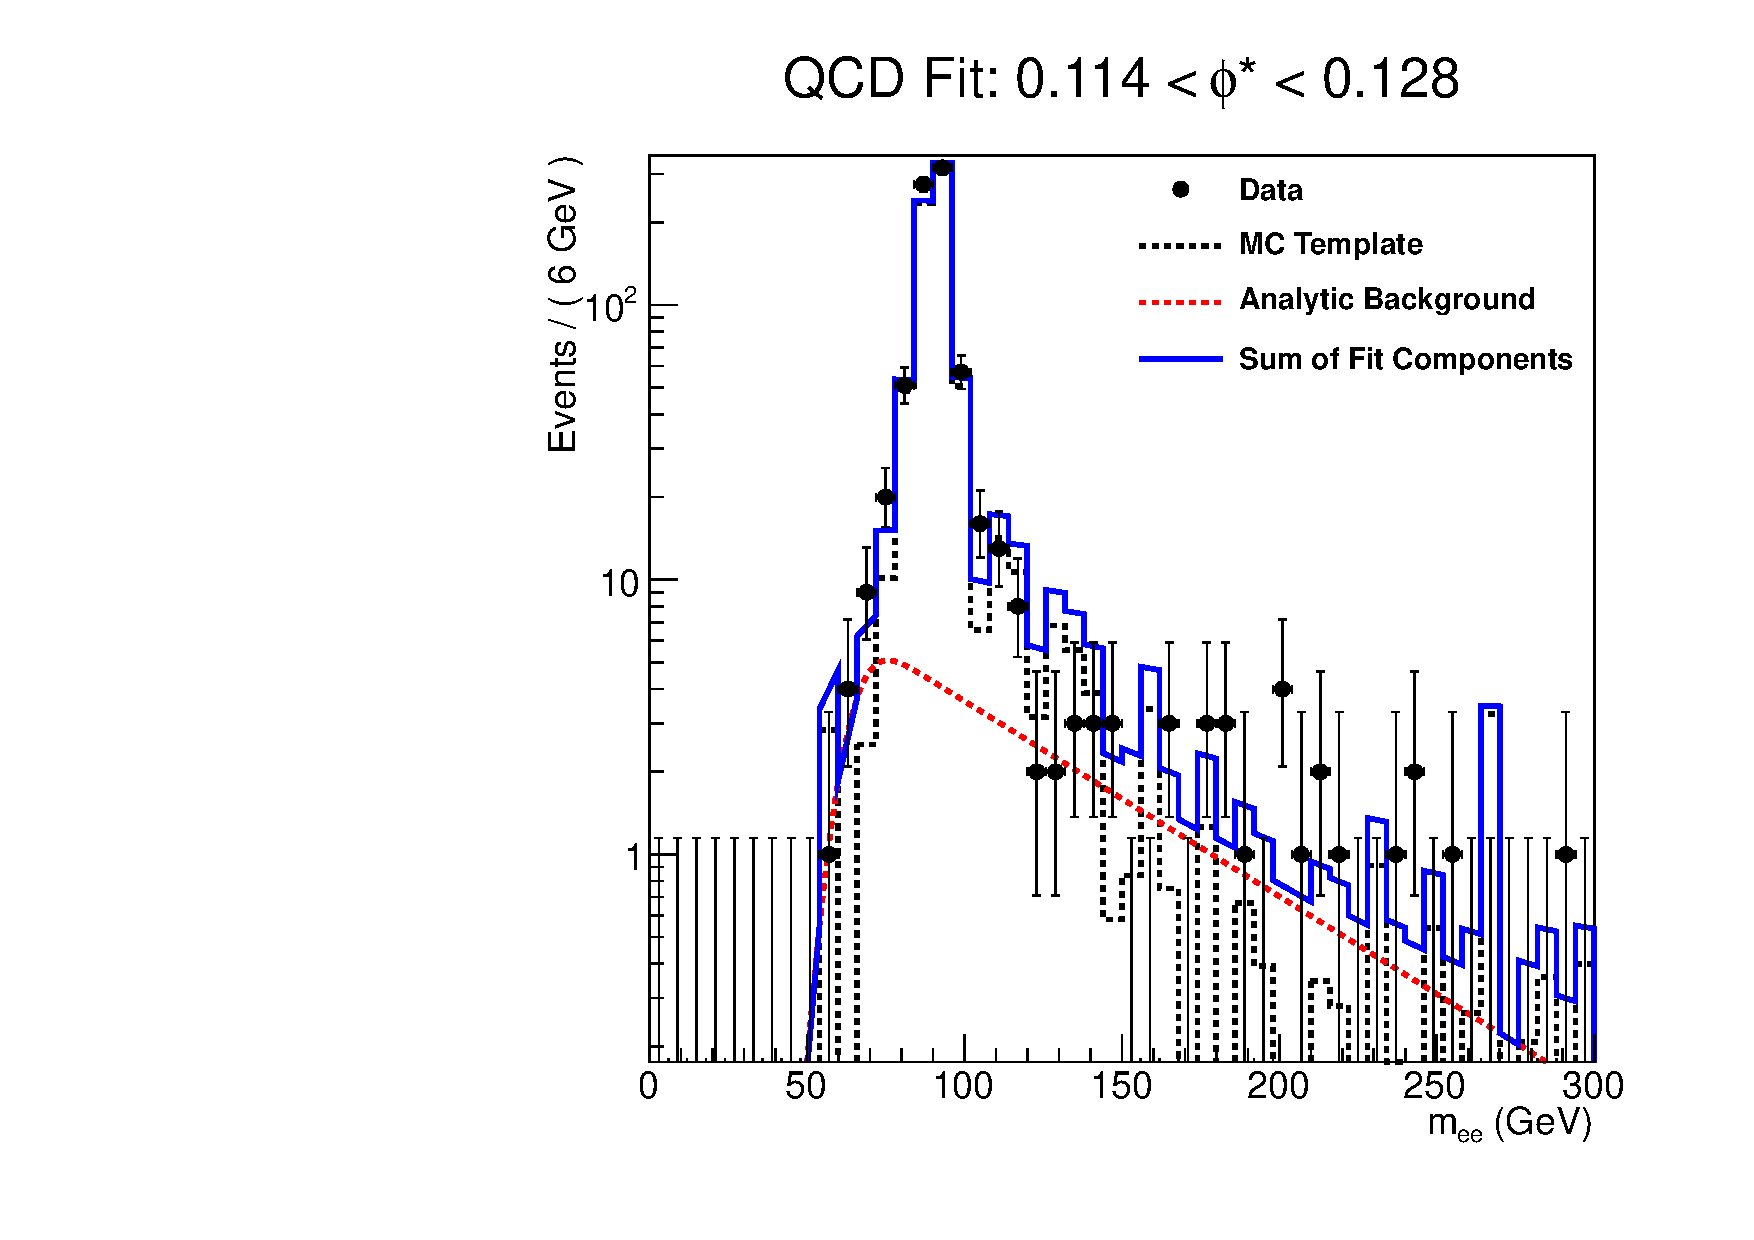
\includegraphics[width=\linewidth]{figures/qcd_fits/qcd_fit_plot_for_19.pdf}
        \label{fig:qcd_fit_19}
    \end{subfigure}%
    \begin{subfigure}[b]{\SideBySidePlotWidth}
        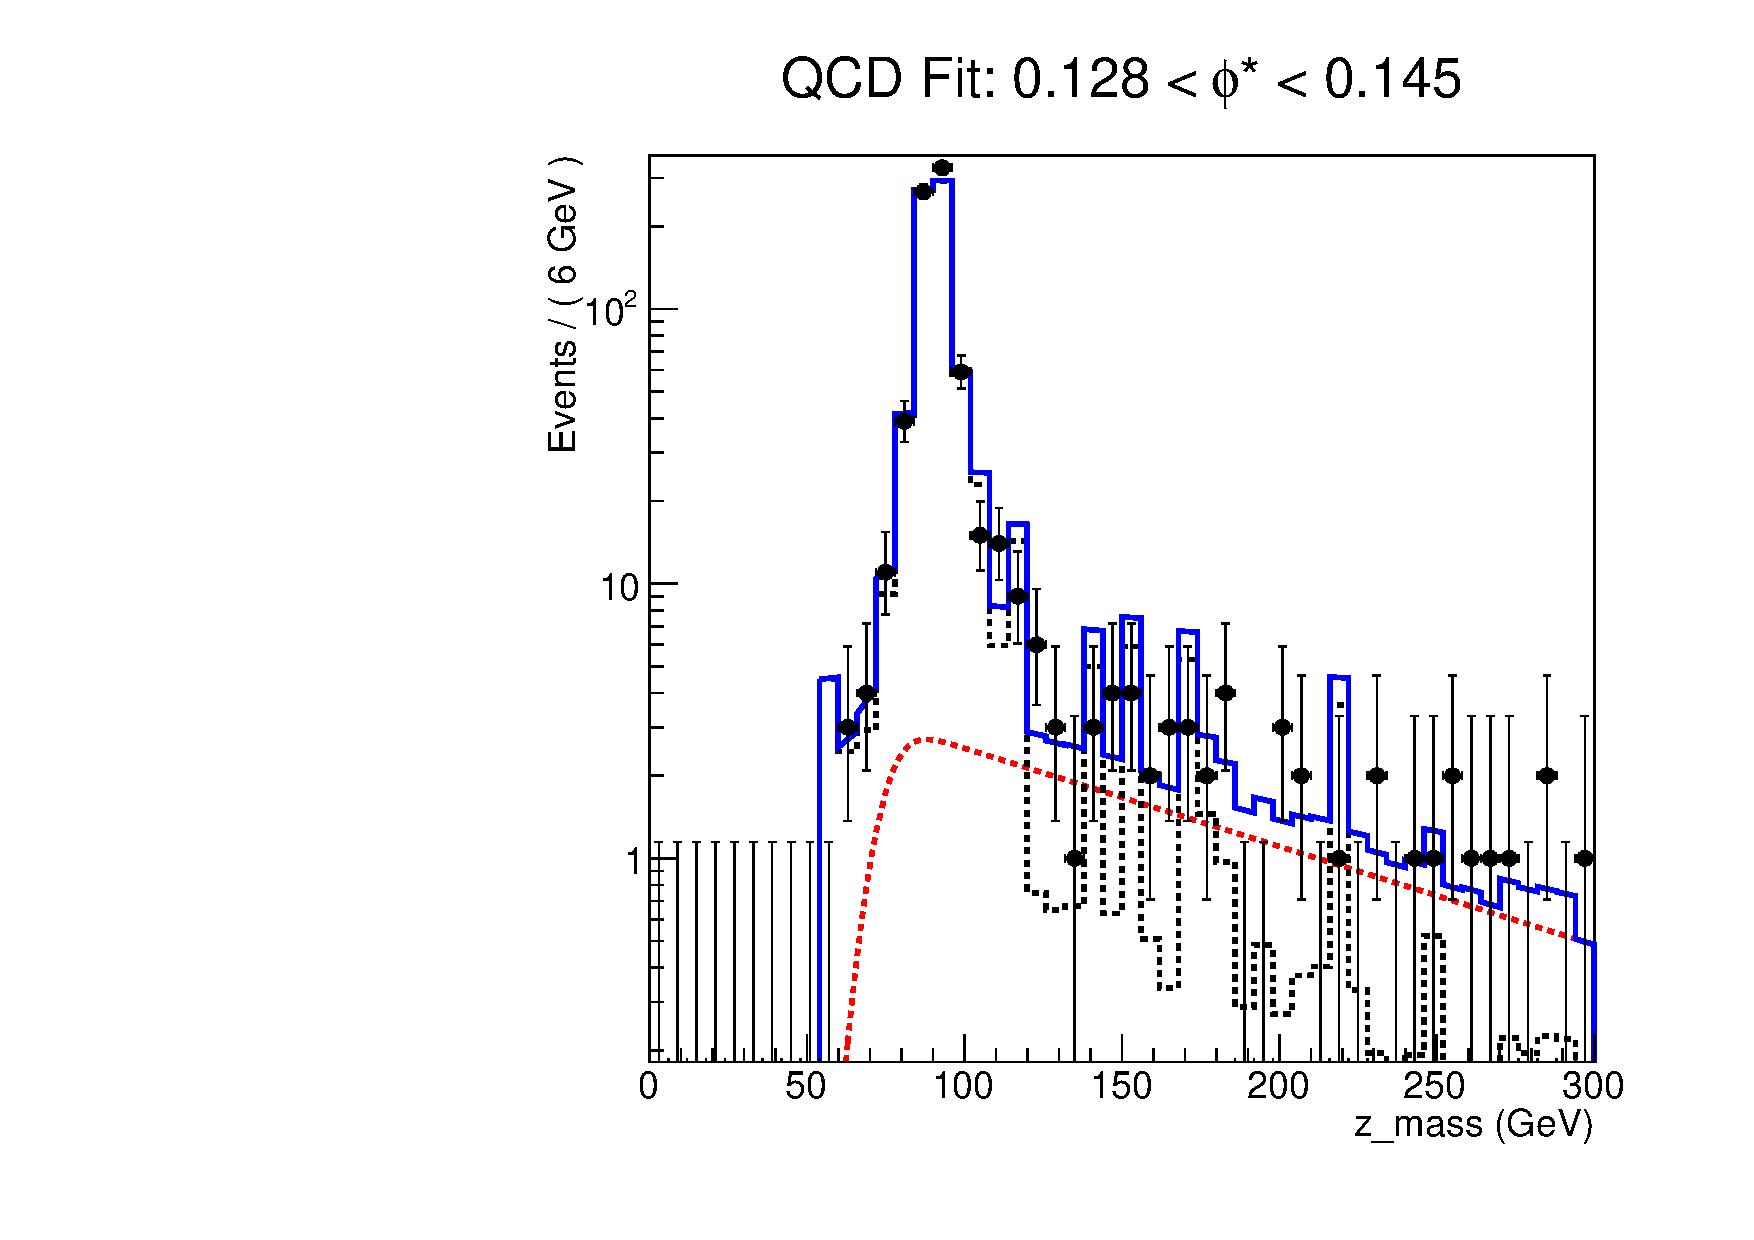
\includegraphics[width=\linewidth]{figures/qcd_fits/qcd_fit_plot_for_20.pdf}
        \label{fig:qcd_fit_20}
    \end{subfigure}
    \caption[
       The \QCDjets and \wjets data-driven background fits for the fifth set of
       four \phistar bins.
    ]{
       The \QCDjets and \wjets data-driven background fits for the fifth set of
       four \phistar bins. The data are shown as points with error bars, MC
       template as a dashed histogram, the analytic background function as the
       dashed line, and the sum of the template and function as a solid
       histogram.
    }
    \label{fig:qcd_many_5}
\end{figure}

\begin{figure}[!htbp]
    \centering
    \begin{subfigure}[b]{\SideBySidePlotWidth}
        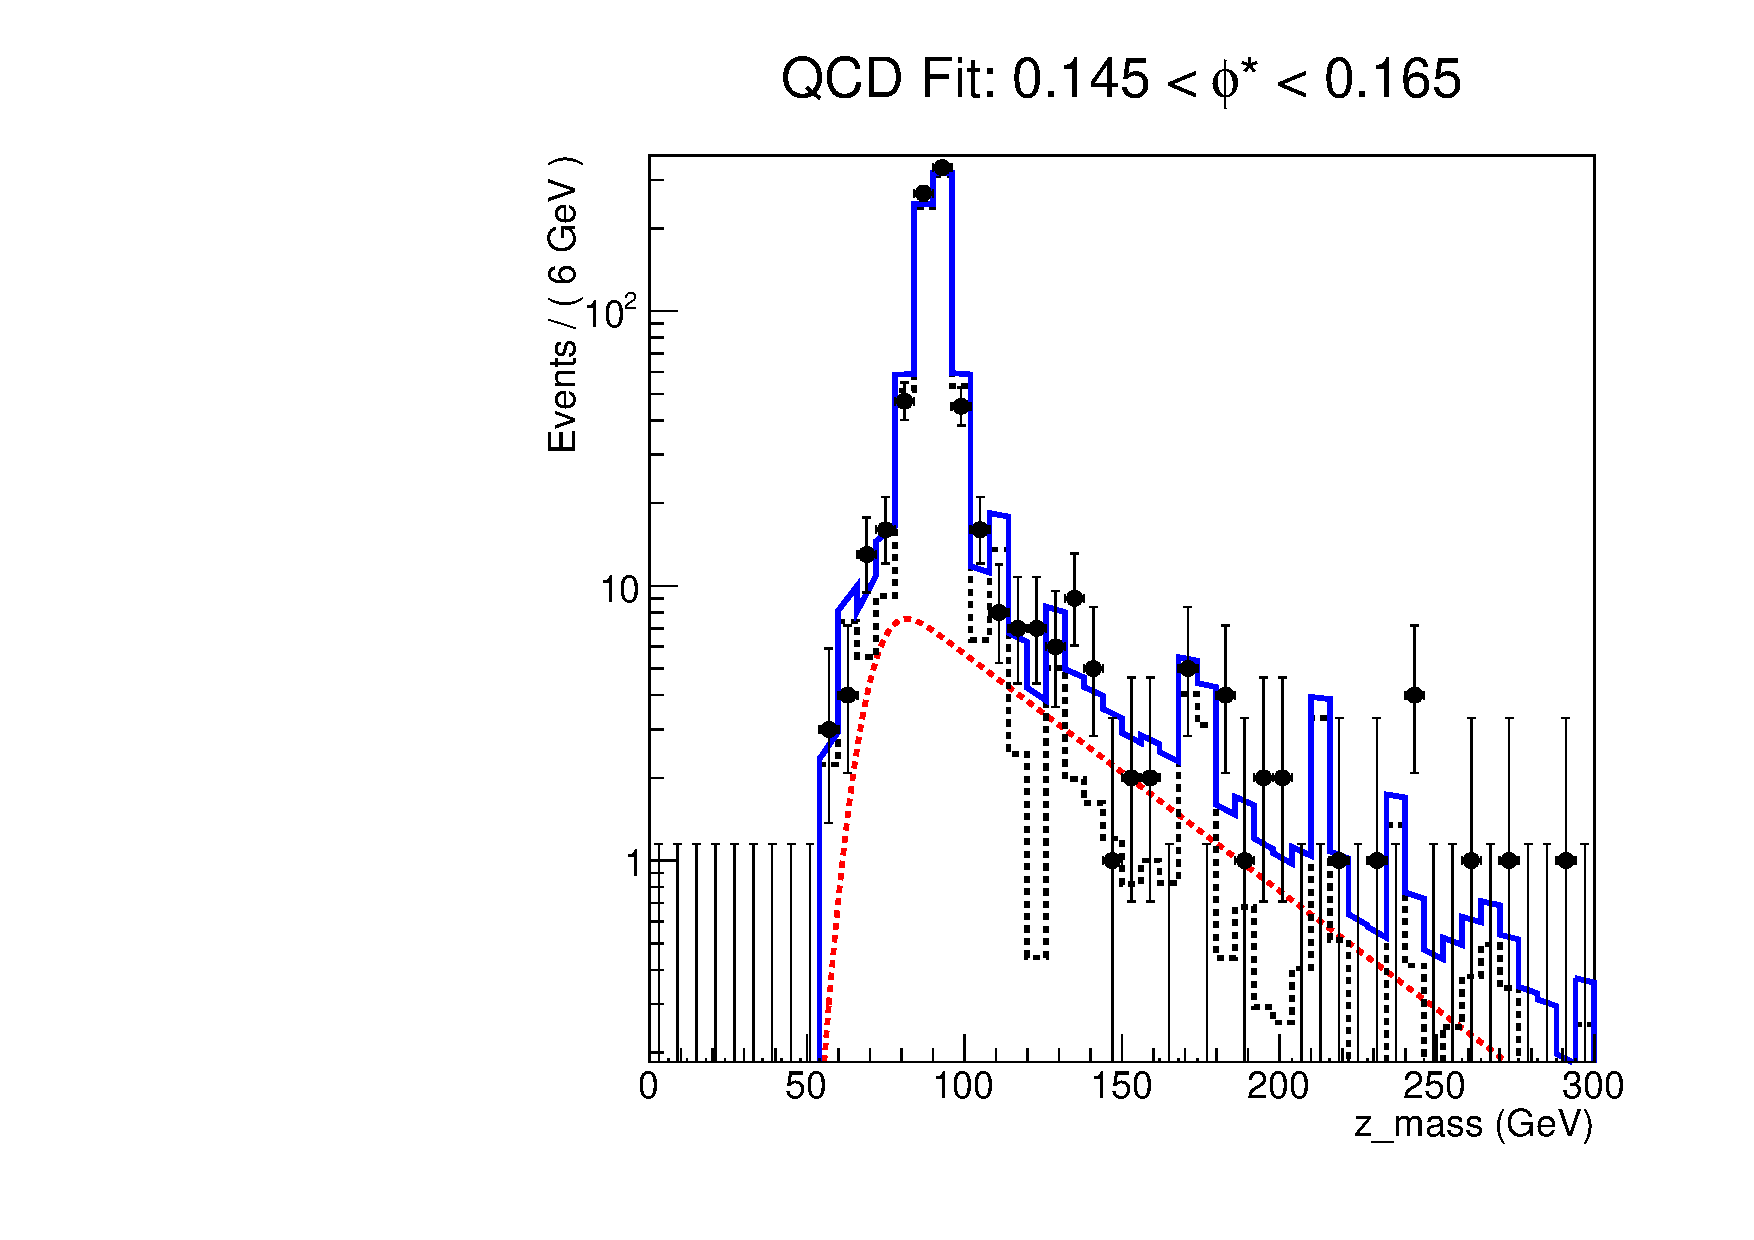
\includegraphics[width=\linewidth]{figures/qcd_fits/qcd_fit_plot_for_21.pdf}
        \label{fig:qcd_fit_21}
    \end{subfigure}%
    % The comment right after suppresses white space that would push the images
    % to new lines
    \begin{subfigure}[b]{\SideBySidePlotWidth}
        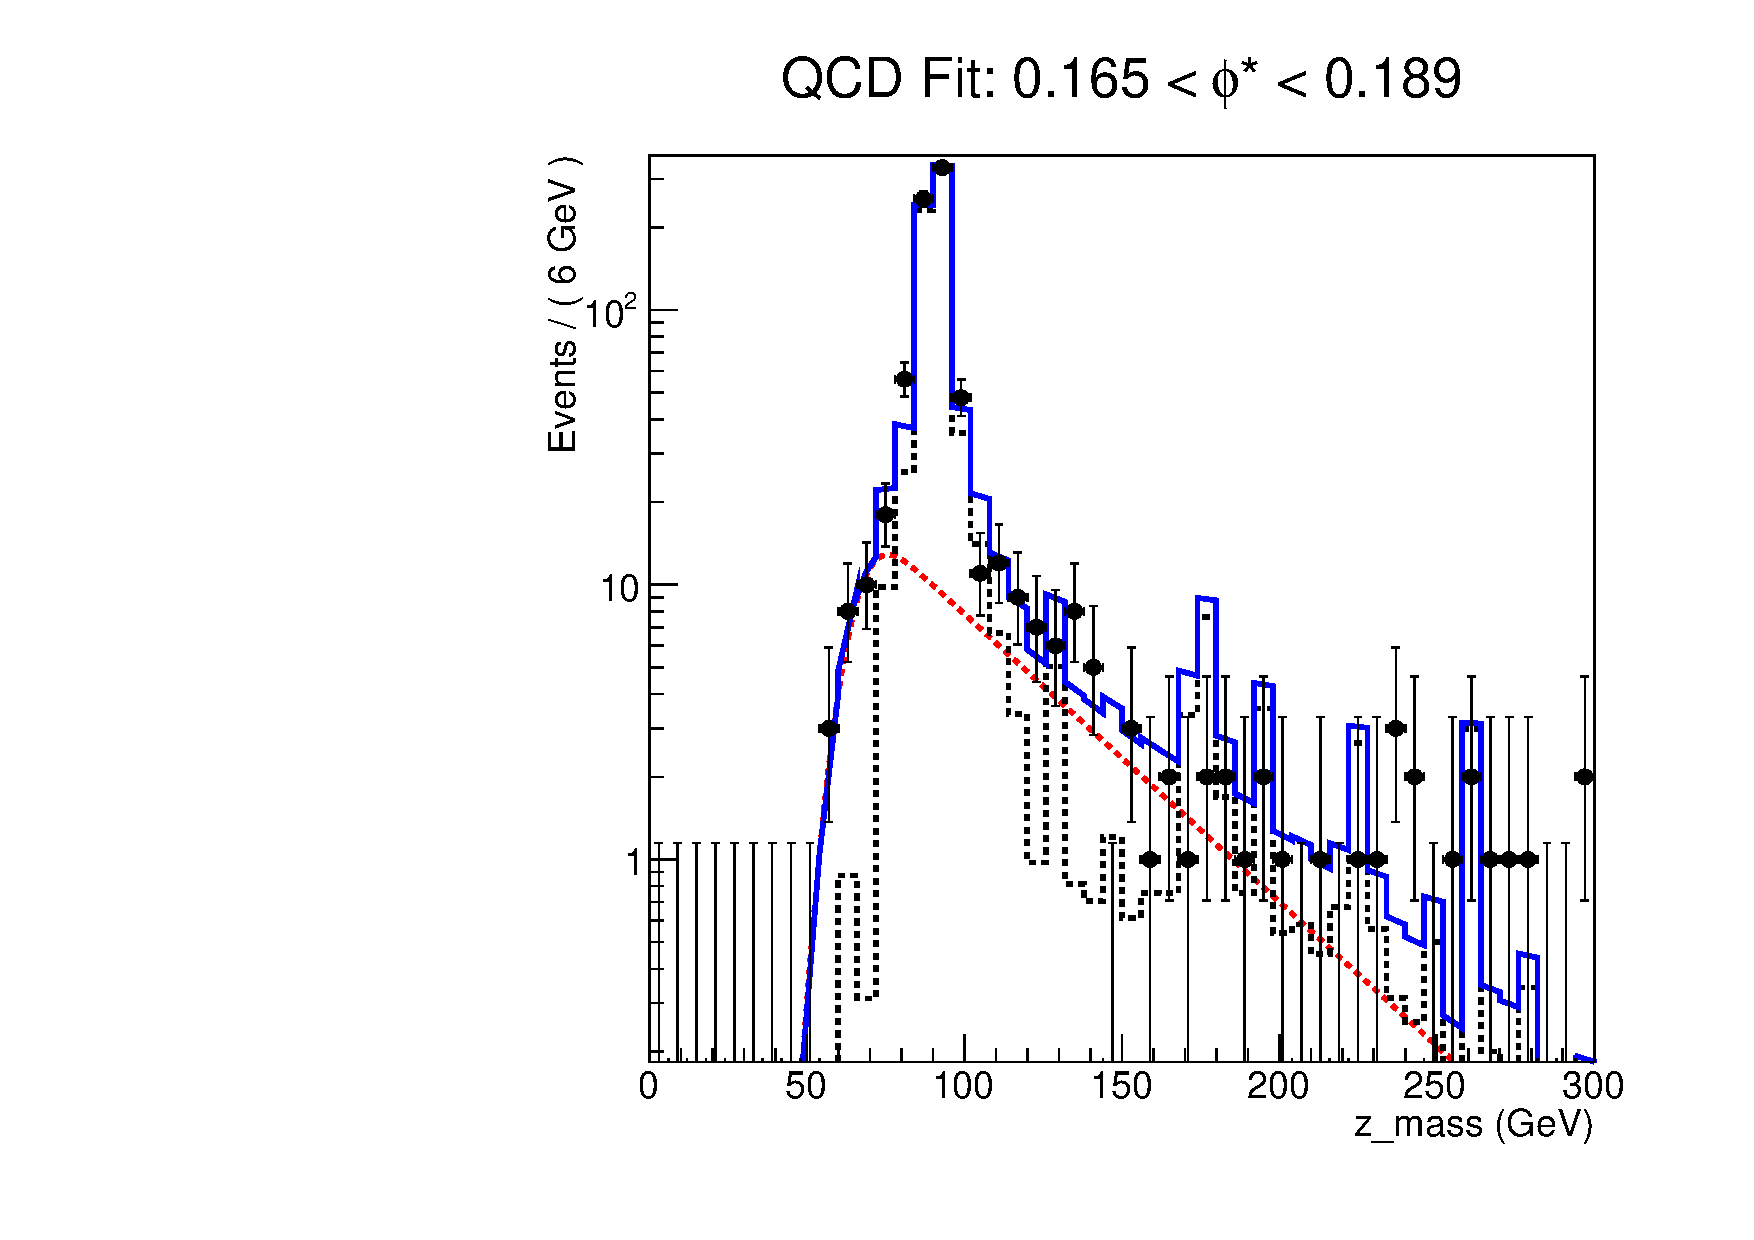
\includegraphics[width=\linewidth]{figures/qcd_fits/qcd_fit_plot_for_22.pdf}
        \label{fig:qcd_fit_22}
    \end{subfigure}
    % New line
    \begin{subfigure}[b]{\SideBySidePlotWidth}
        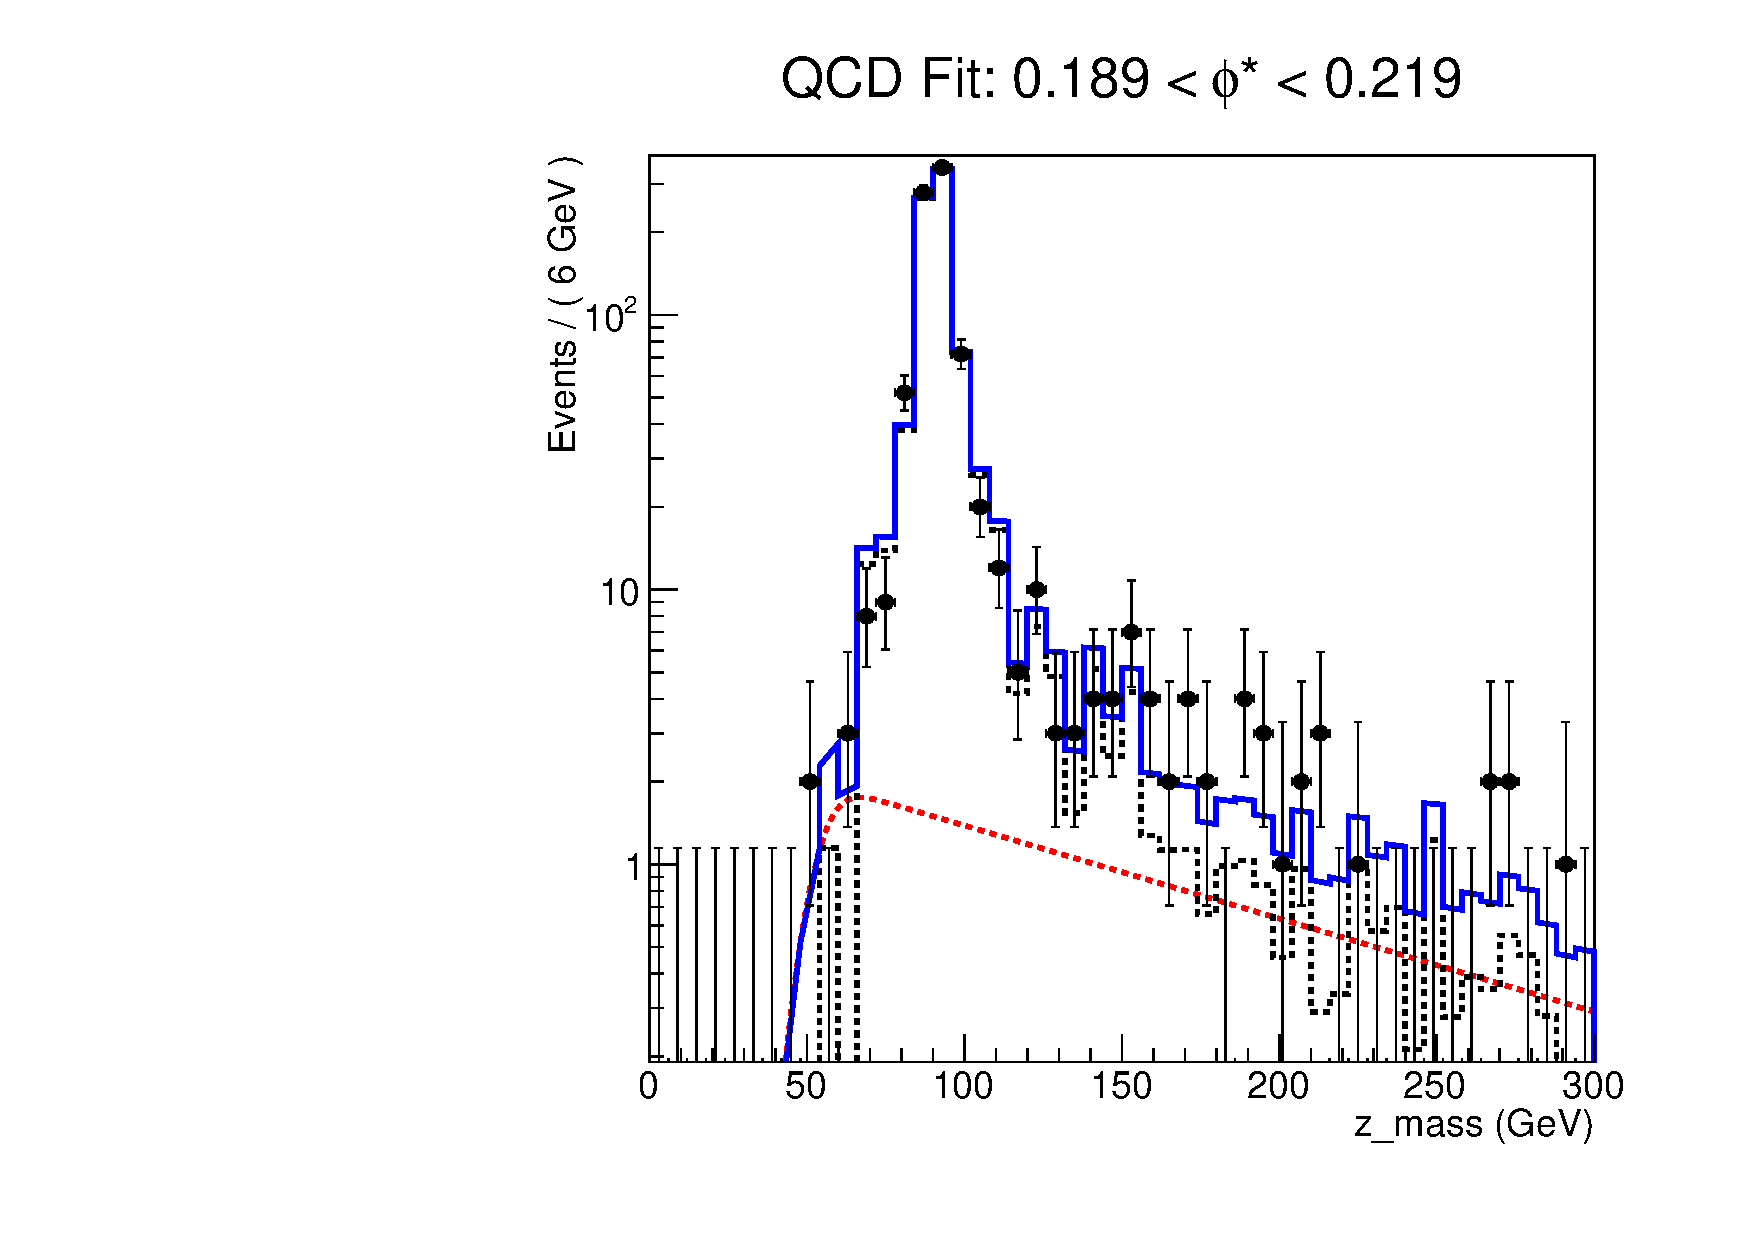
\includegraphics[width=\linewidth]{figures/qcd_fits/qcd_fit_plot_for_23.pdf}
        \label{fig:qcd_fit_23}
    \end{subfigure}%
    \begin{subfigure}[b]{\SideBySidePlotWidth}
        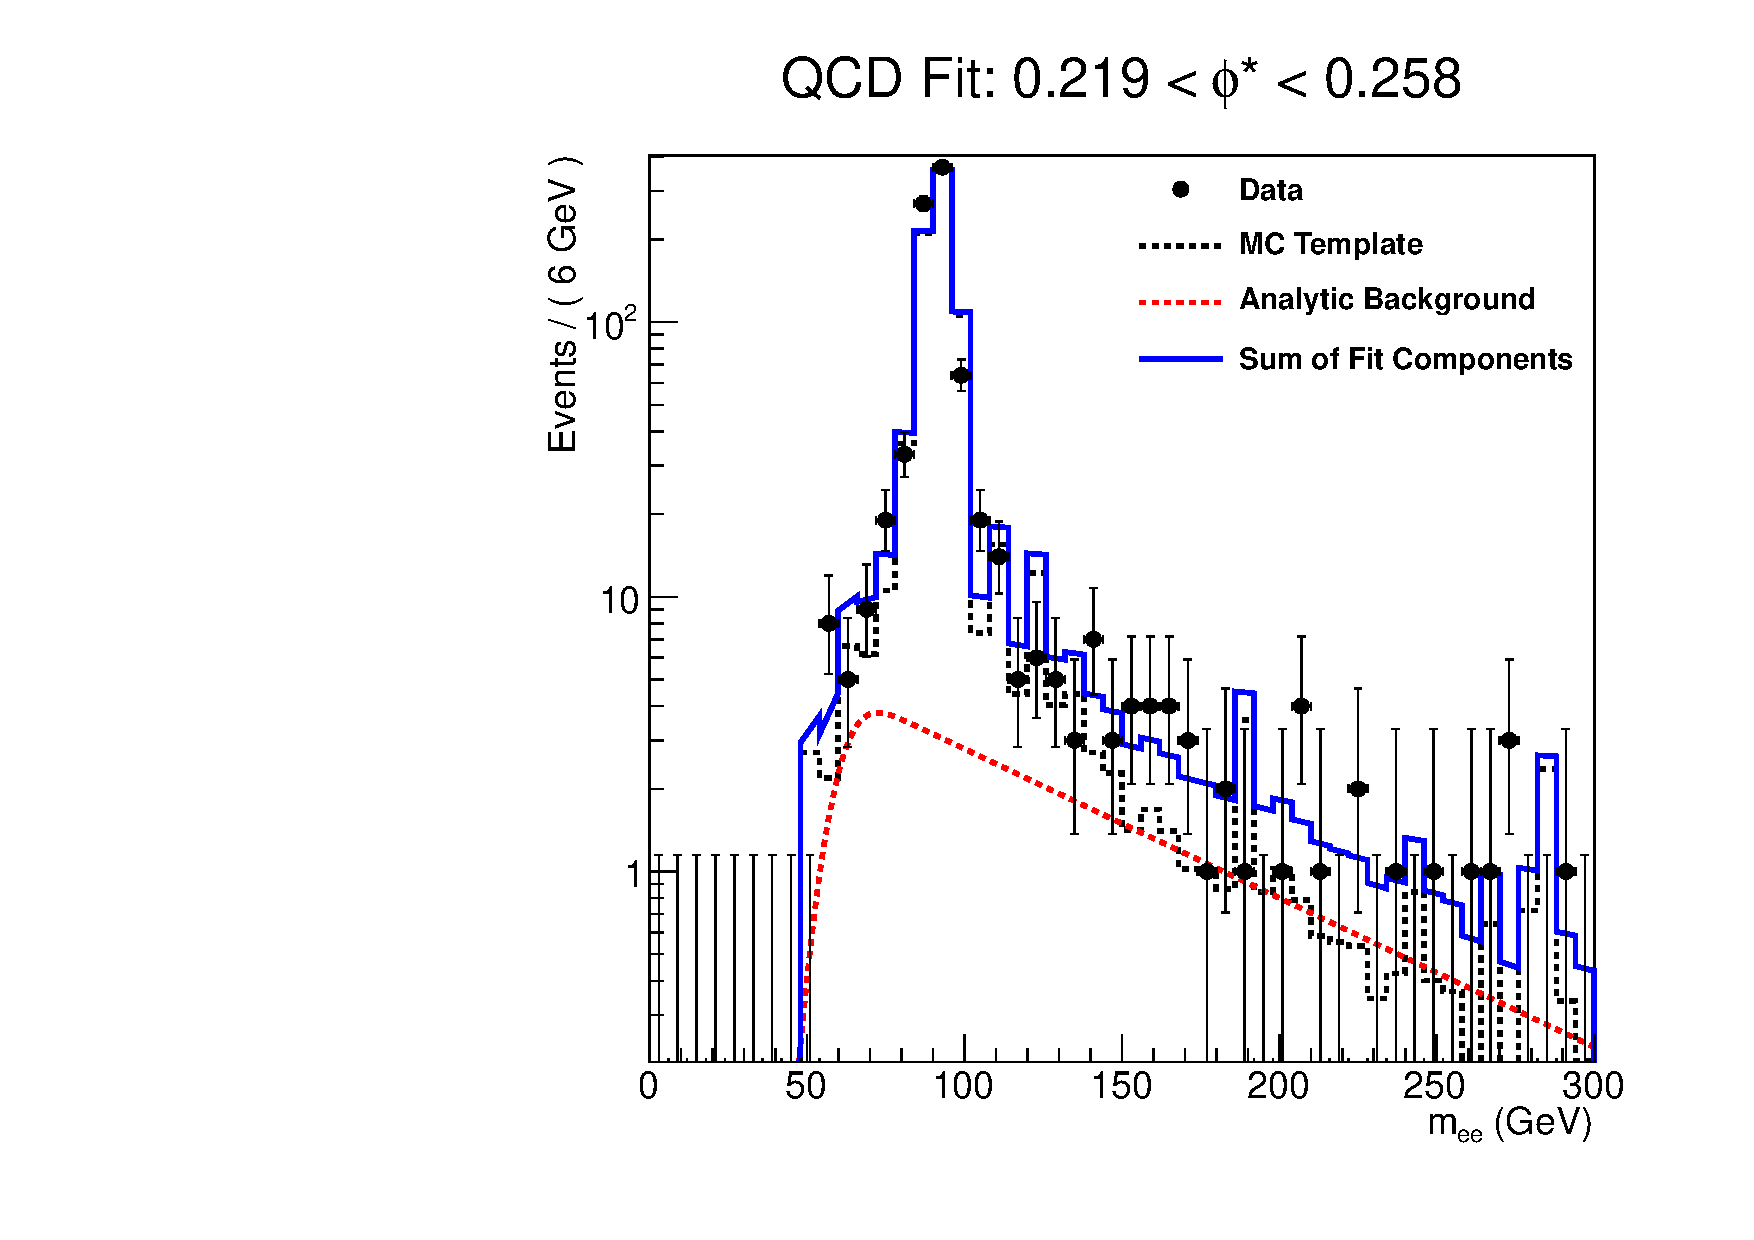
\includegraphics[width=\linewidth]{figures/qcd_fits/qcd_fit_plot_for_24.pdf}
        \label{fig:qcd_fit_24}
    \end{subfigure}
    \caption[
       The \QCDjets and \wjets data-driven background fits for the sixth set of
       four \phistar bins.
    ]{
       The \QCDjets and \wjets data-driven background fits for the sixth set of
       four \phistar bins. The data are shown as points with error bars, MC
       template as a dashed histogram, the analytic background function as the
       dashed line, and the sum of the template and function as a solid
       histogram.
    }
    \label{fig:qcd_many_6}
\end{figure}

\begin{figure}[!htbp]
    \centering
    \begin{subfigure}[b]{\SideBySidePlotWidth}
        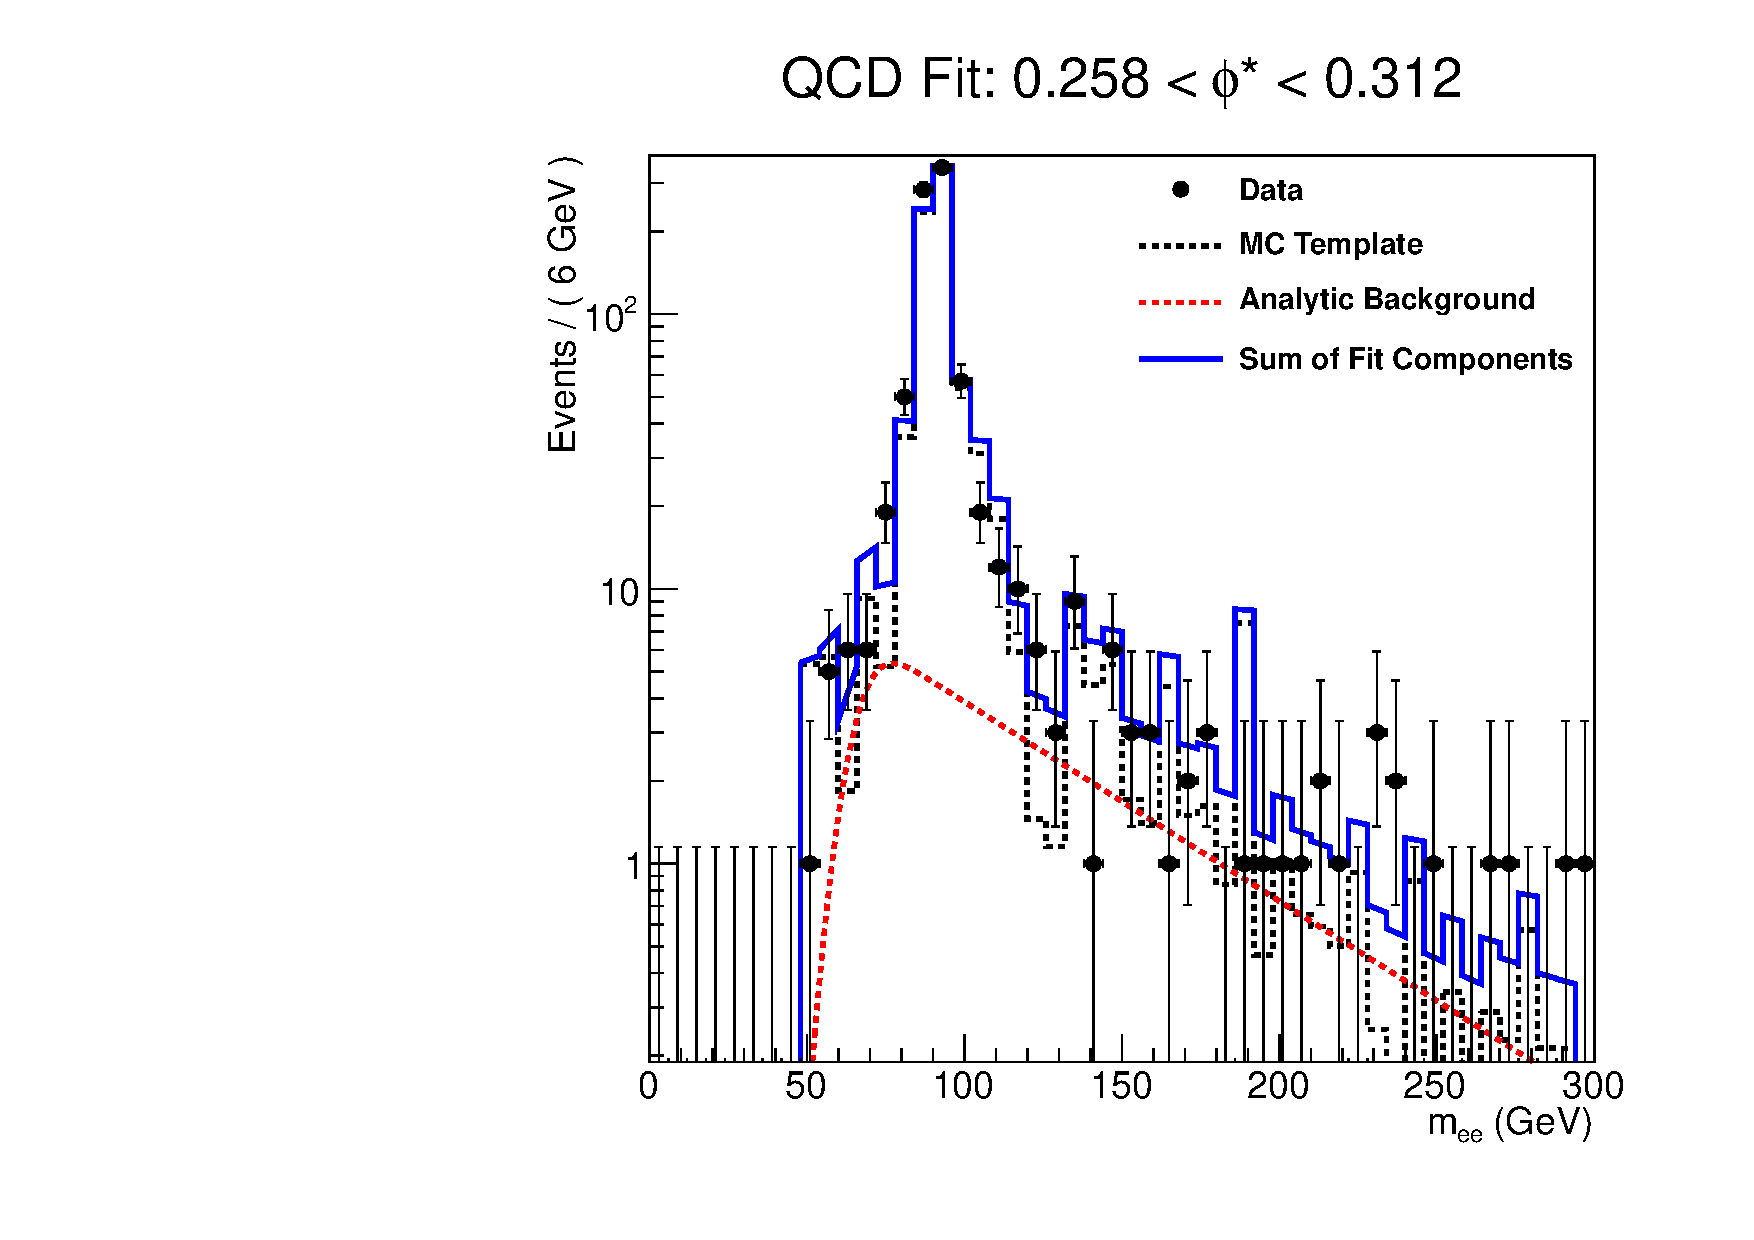
\includegraphics[width=\linewidth]{figures/qcd_fits/qcd_fit_plot_for_25.pdf}
        \label{fig:qcd_fit_25}
    \end{subfigure}%
    % The comment right after suppresses white space that would push the images
    % to new lines
    \begin{subfigure}[b]{\SideBySidePlotWidth}
        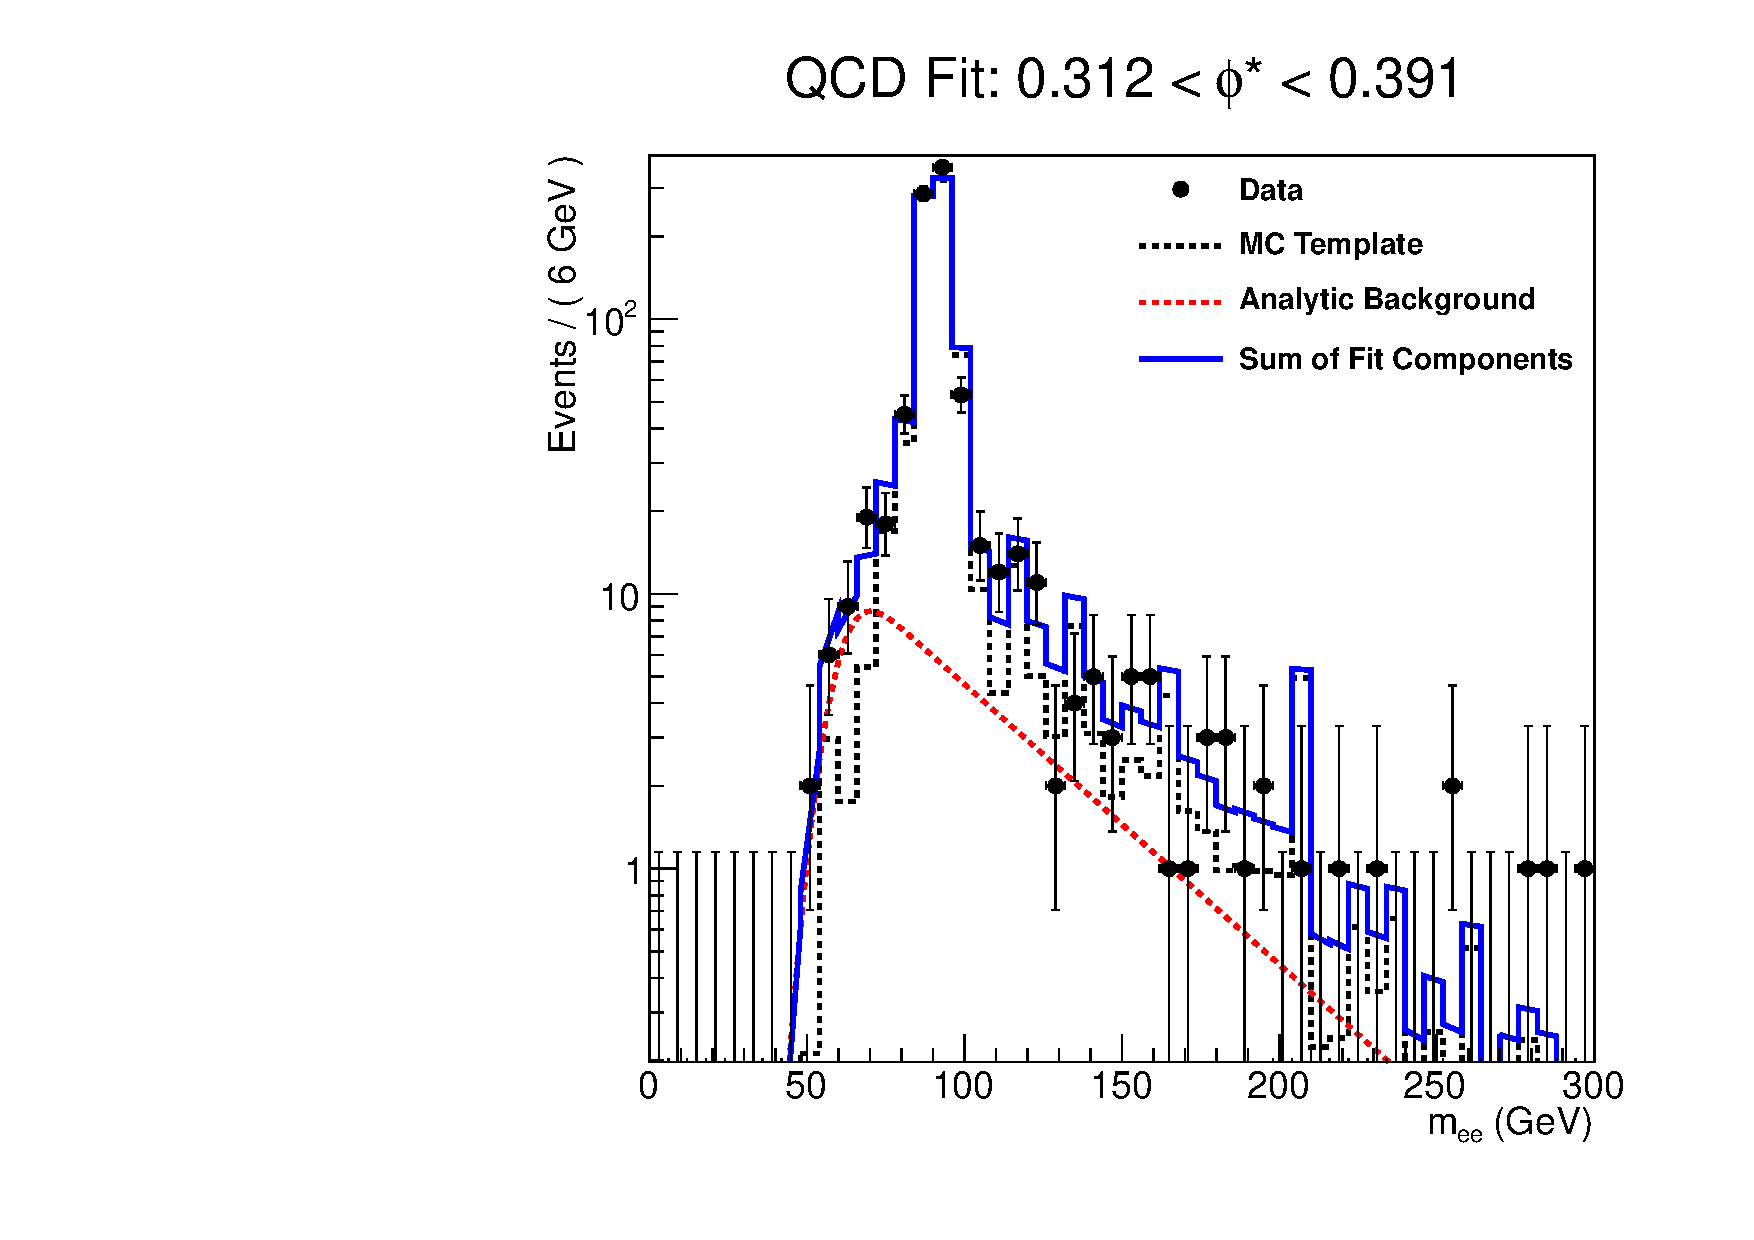
\includegraphics[width=\linewidth]{figures/qcd_fits/qcd_fit_plot_for_26.pdf}
        \label{fig:qcd_fit_26}
    \end{subfigure}
    % New line
    \begin{subfigure}[b]{\SideBySidePlotWidth}
        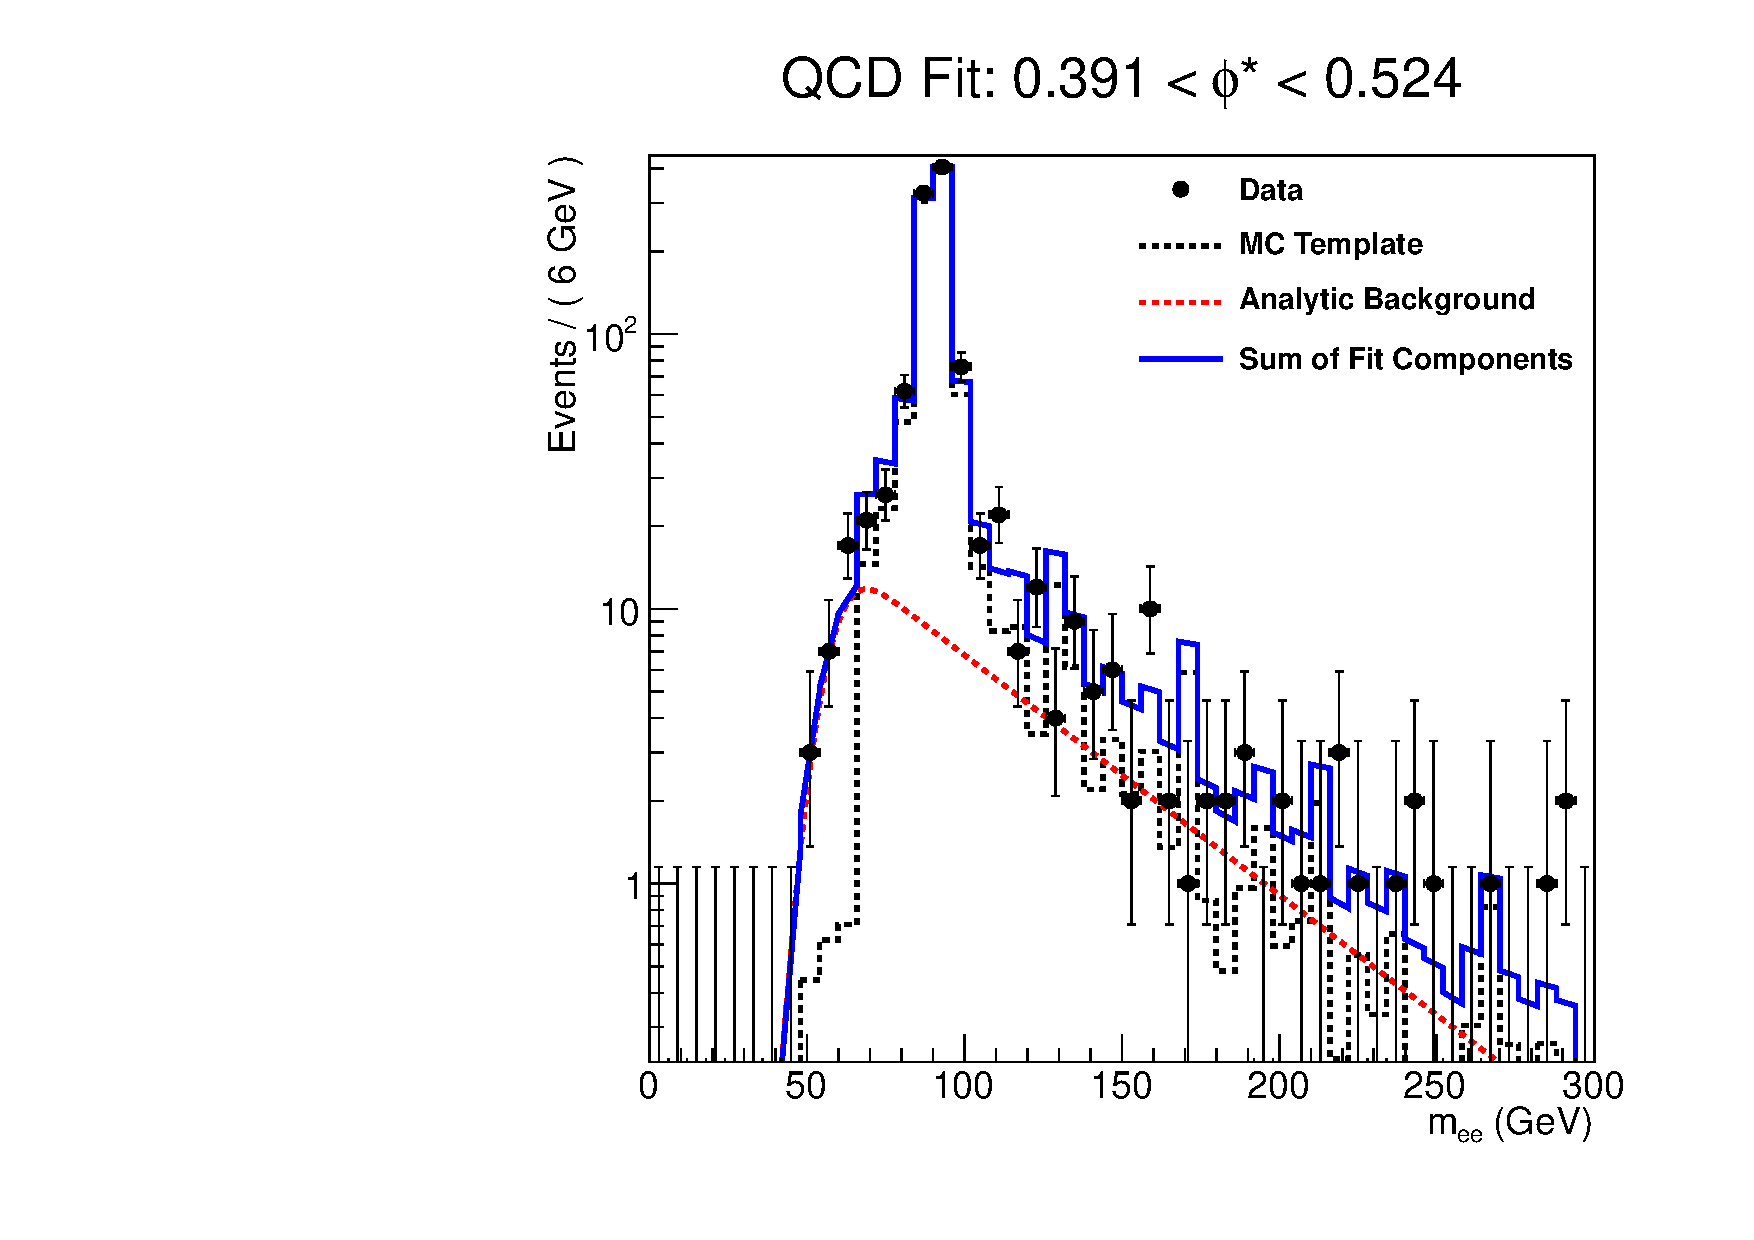
\includegraphics[width=\linewidth]{figures/qcd_fits/qcd_fit_plot_for_27.pdf}
        \label{fig:qcd_fit_27}
    \end{subfigure}%
    \begin{subfigure}[b]{\SideBySidePlotWidth}
        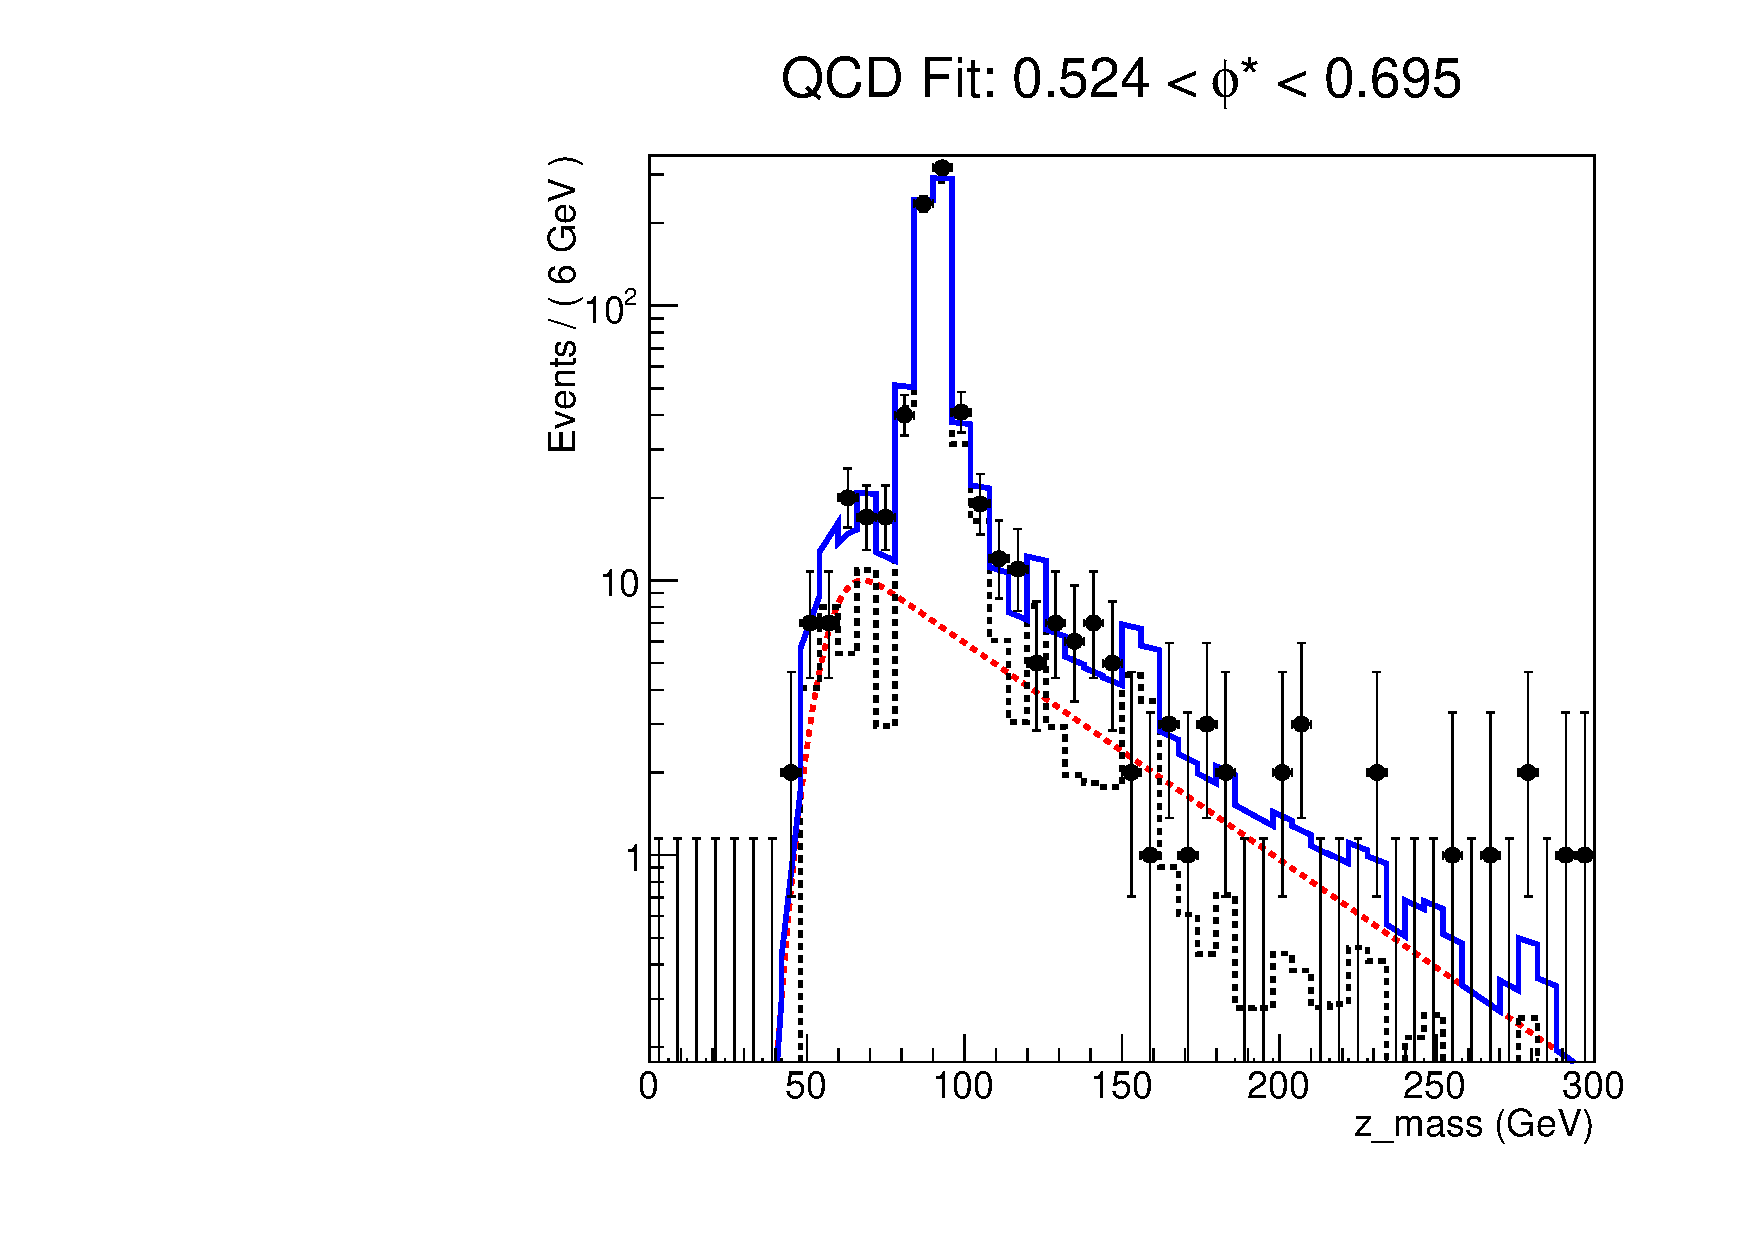
\includegraphics[width=\linewidth]{figures/qcd_fits/qcd_fit_plot_for_28.pdf}
        \label{fig:qcd_fit_28}
    \end{subfigure}
    \caption[
       The \QCDjets and \wjets data-driven background fits for the seventh set
       of four \phistar bins.
    ]{
       The \QCDjets and \wjets data-driven background fits for the seventh set
       of four \phistar bins. The data are shown as points with error bars, MC
       template as a dashed histogram, the analytic background function as the
       dashed line, and the sum of the template and function as a solid
       histogram.
    }
    \label{fig:qcd_many_7}
\end{figure}

\begin{figure}[!htbp]
    \centering
    \begin{subfigure}[b]{\SideBySidePlotWidth}
        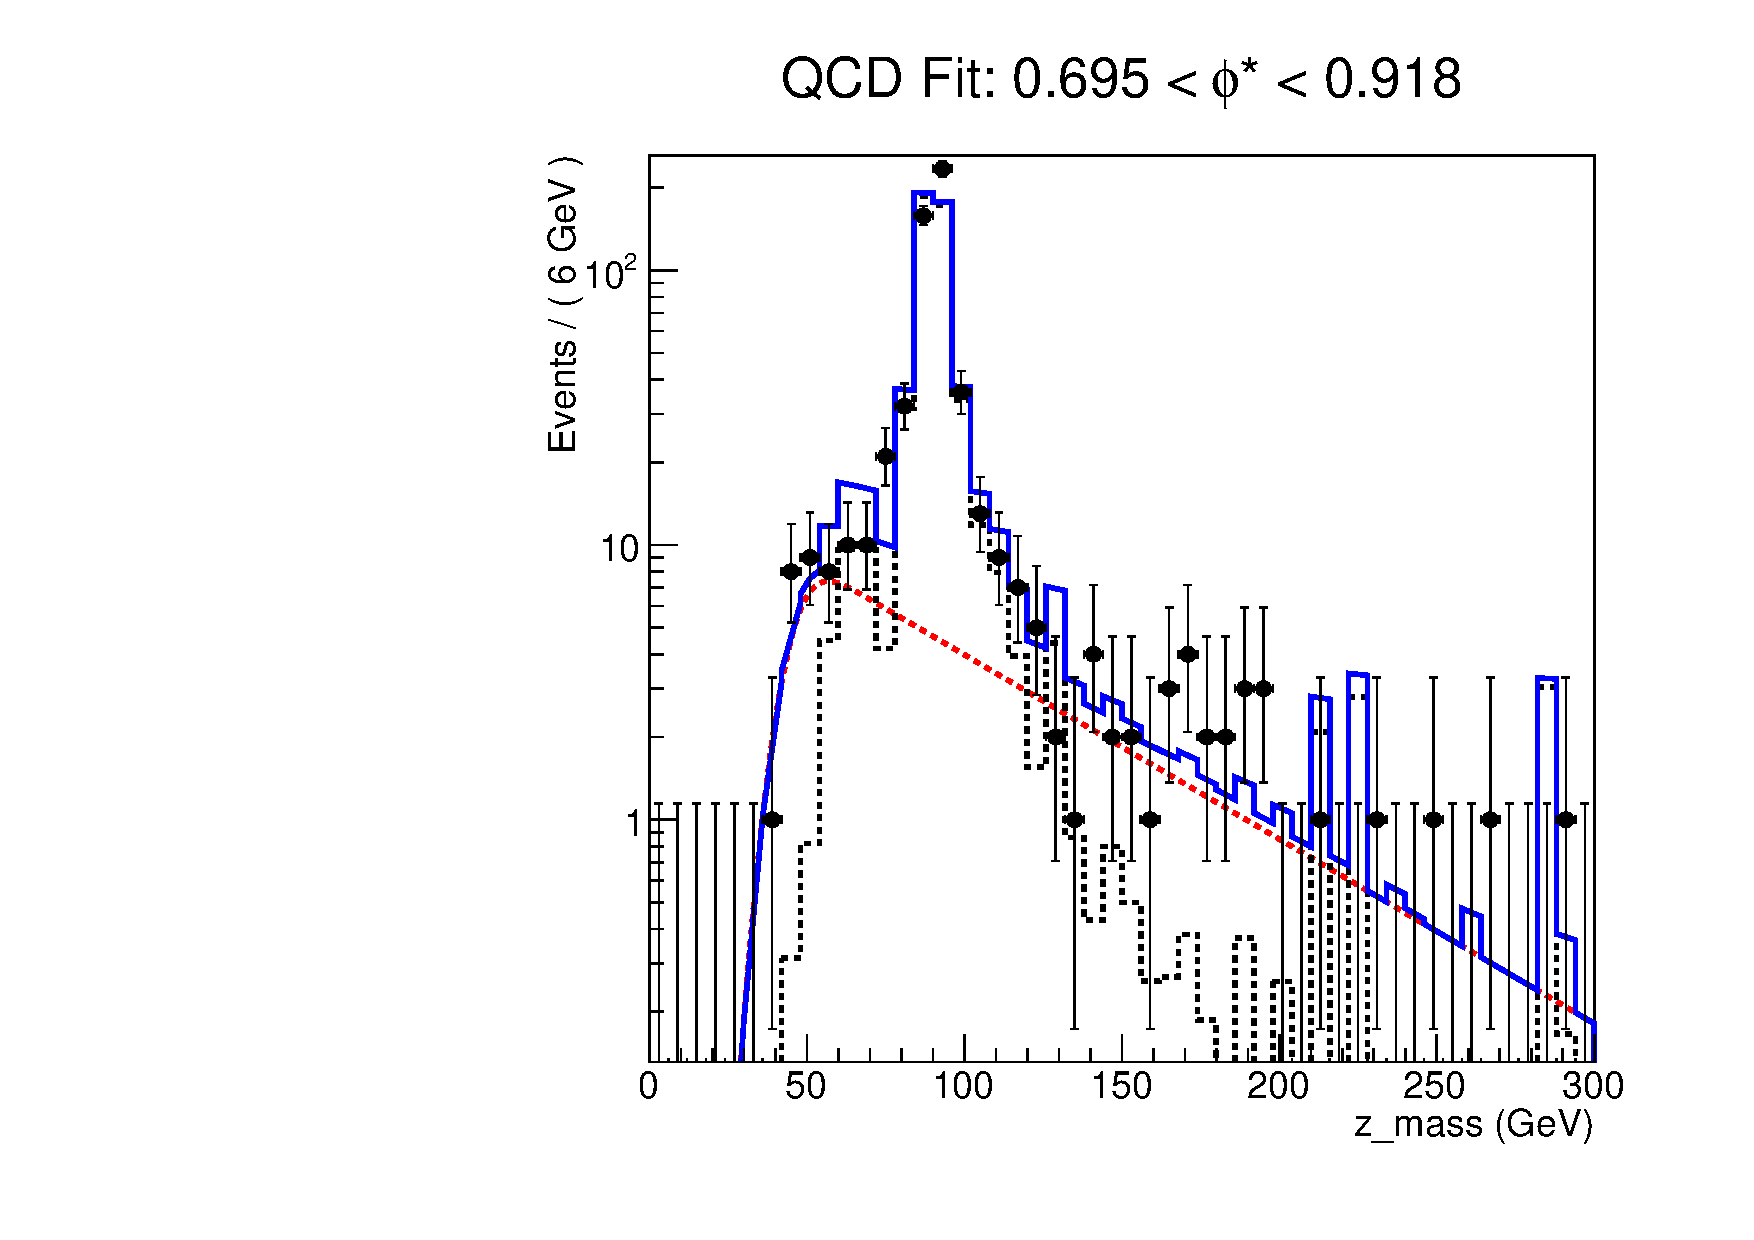
\includegraphics[width=\linewidth]{figures/qcd_fits/qcd_fit_plot_for_29.pdf}
        \label{fig:qcd_fit_29}
    \end{subfigure}%
    % The comment right after suppresses white space that would push the images
    % to new lines
    \begin{subfigure}[b]{\SideBySidePlotWidth}
        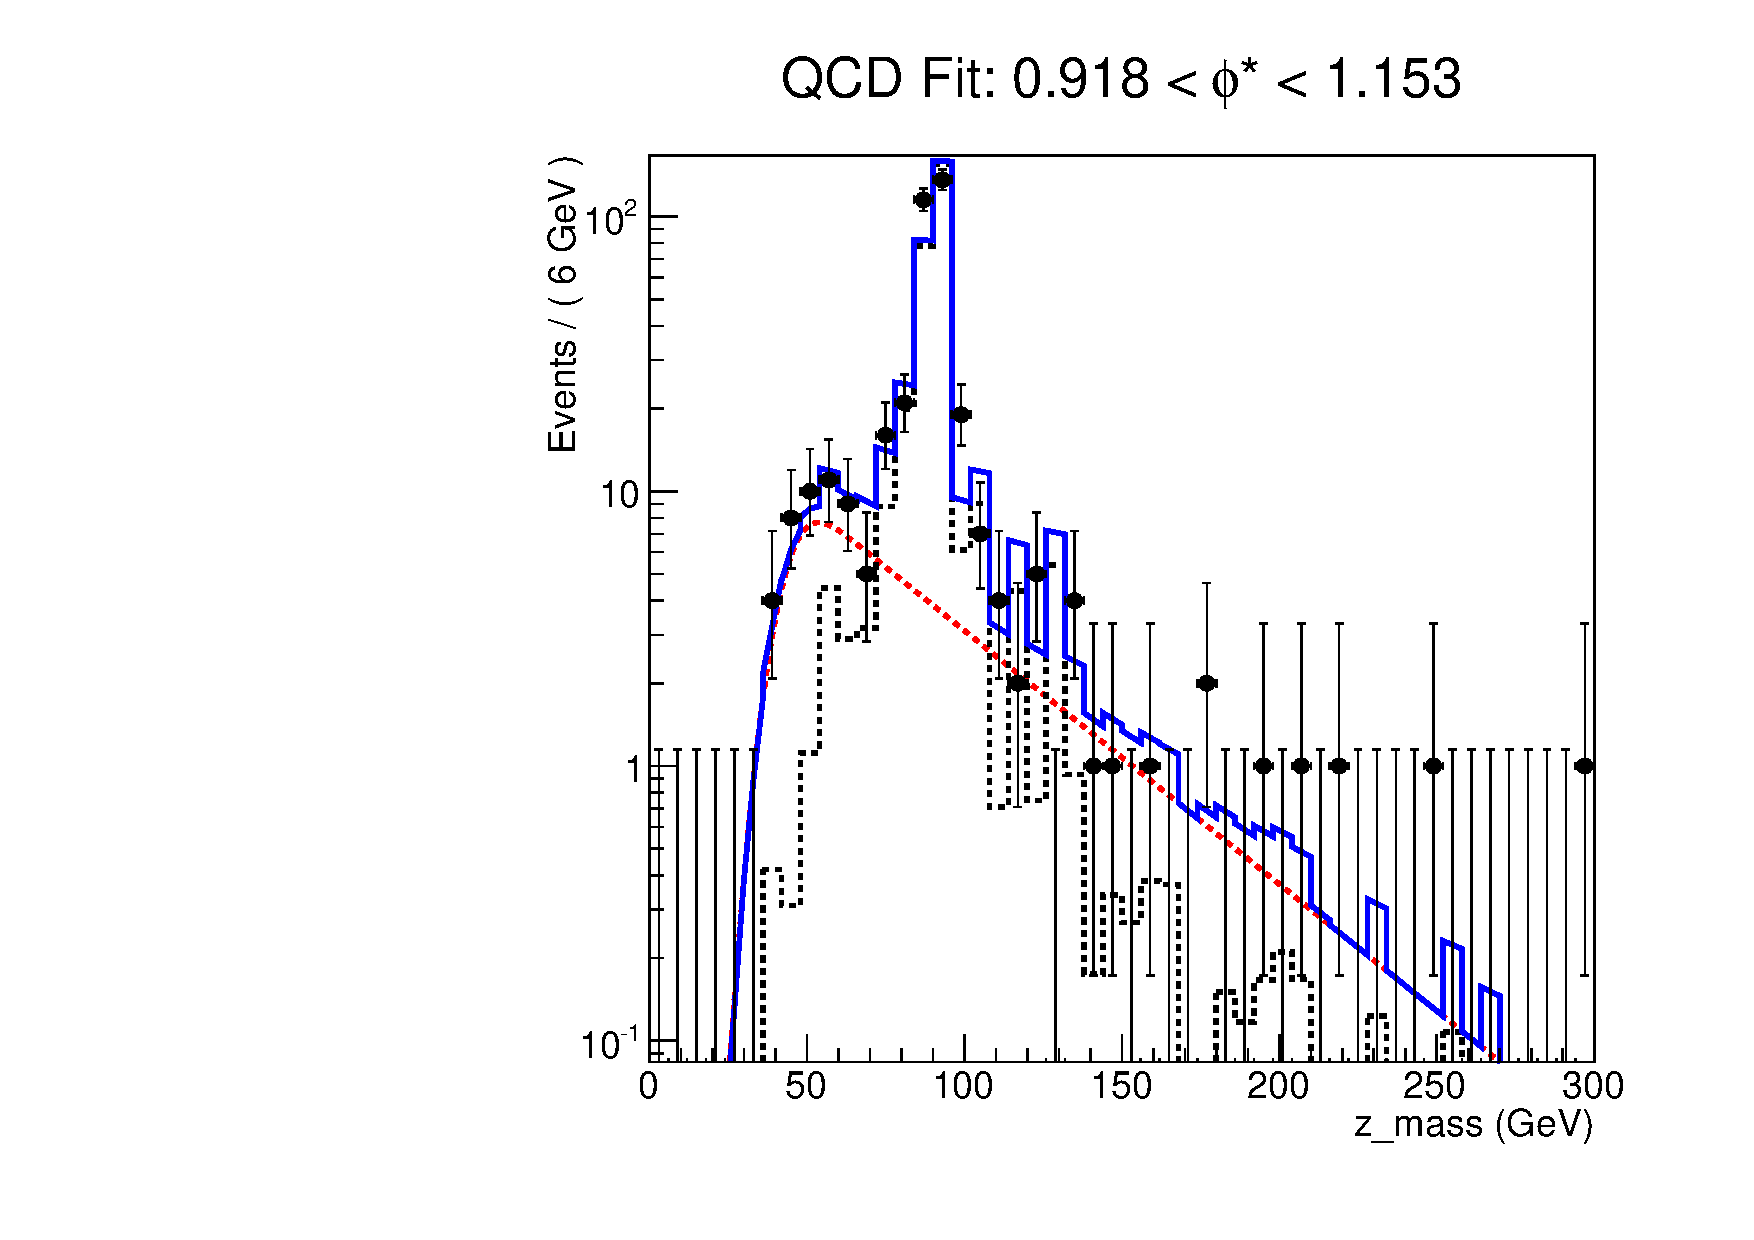
\includegraphics[width=\linewidth]{figures/qcd_fits/qcd_fit_plot_for_30.pdf}
        \label{fig:qcd_fit_30}
    \end{subfigure}
    % New line
    \begin{subfigure}[b]{\SideBySidePlotWidth}
        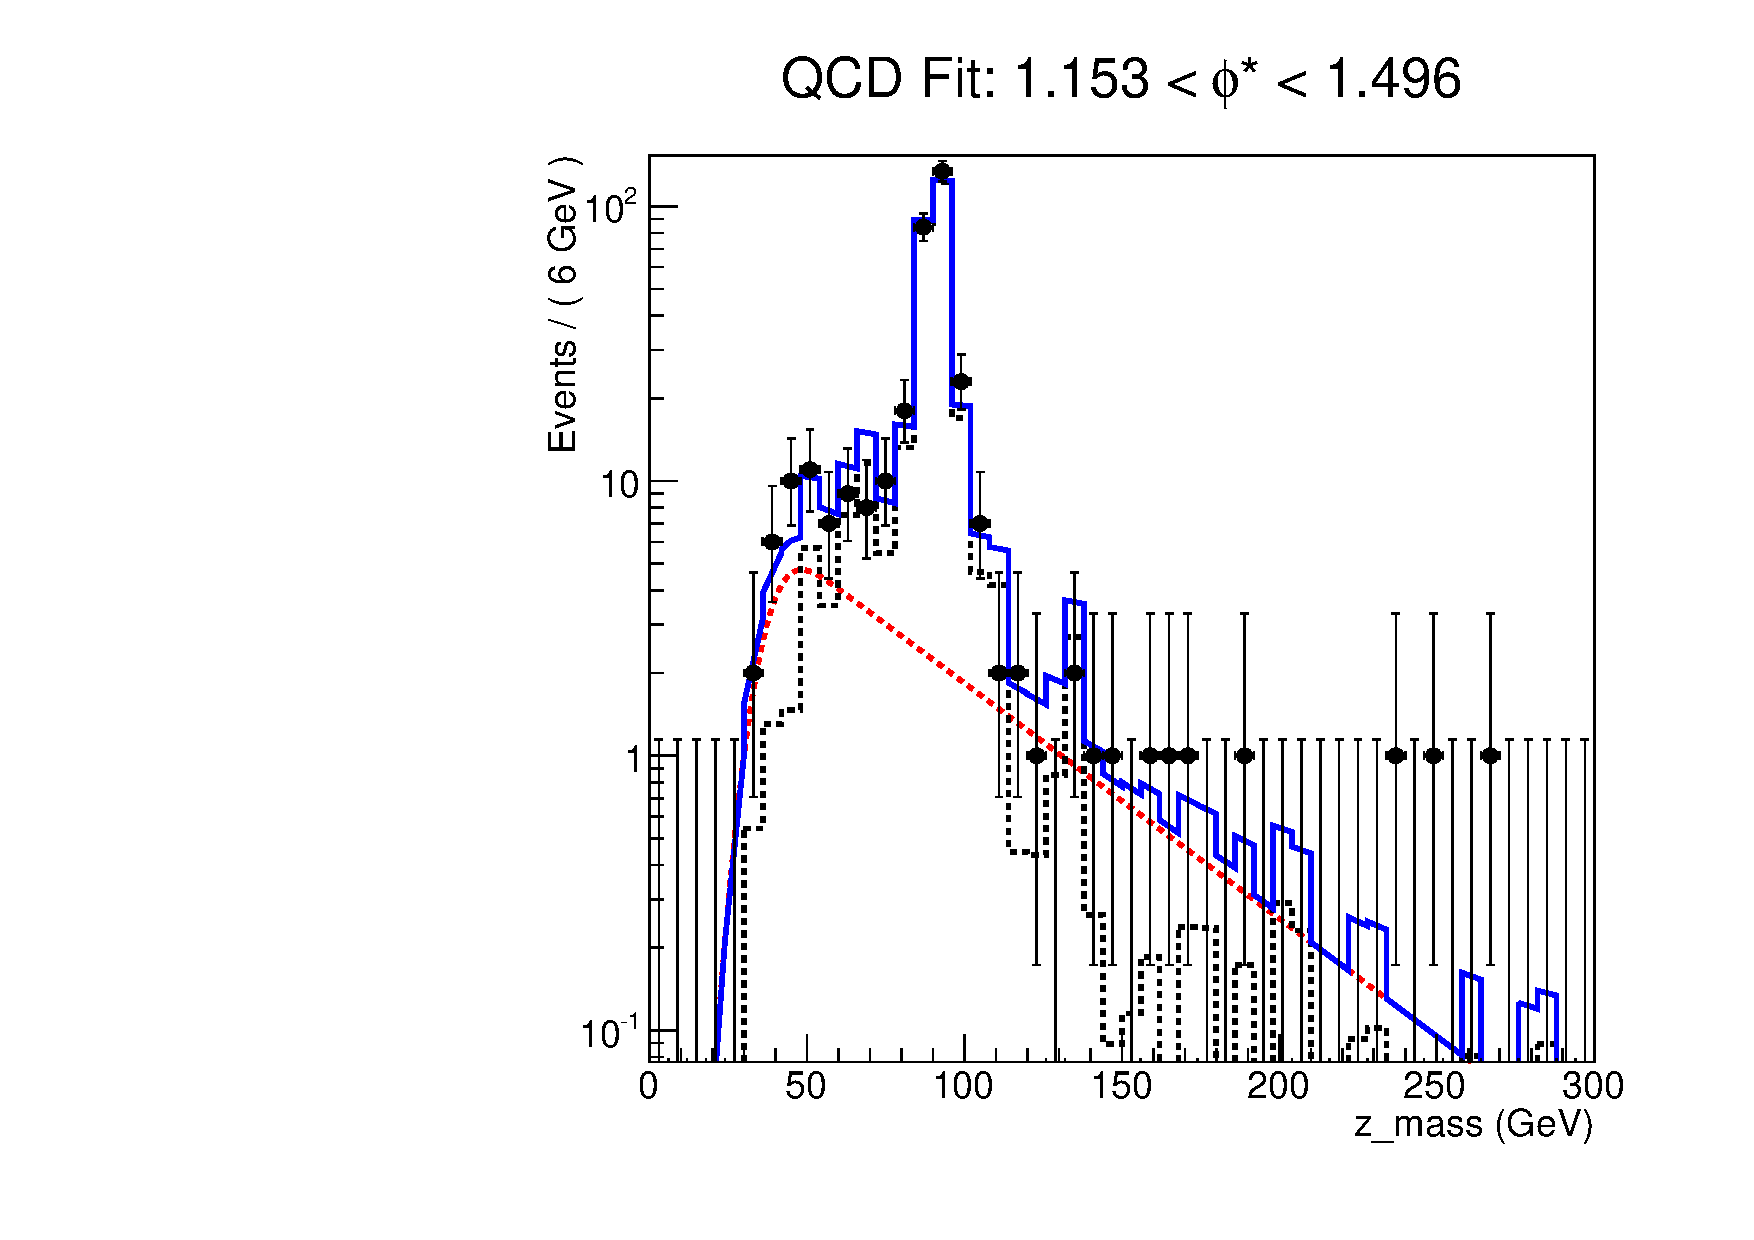
\includegraphics[width=\linewidth]{figures/qcd_fits/qcd_fit_plot_for_31.pdf}
        \label{fig:qcd_fit_31}
    \end{subfigure}%
    \begin{subfigure}[b]{\SideBySidePlotWidth}
        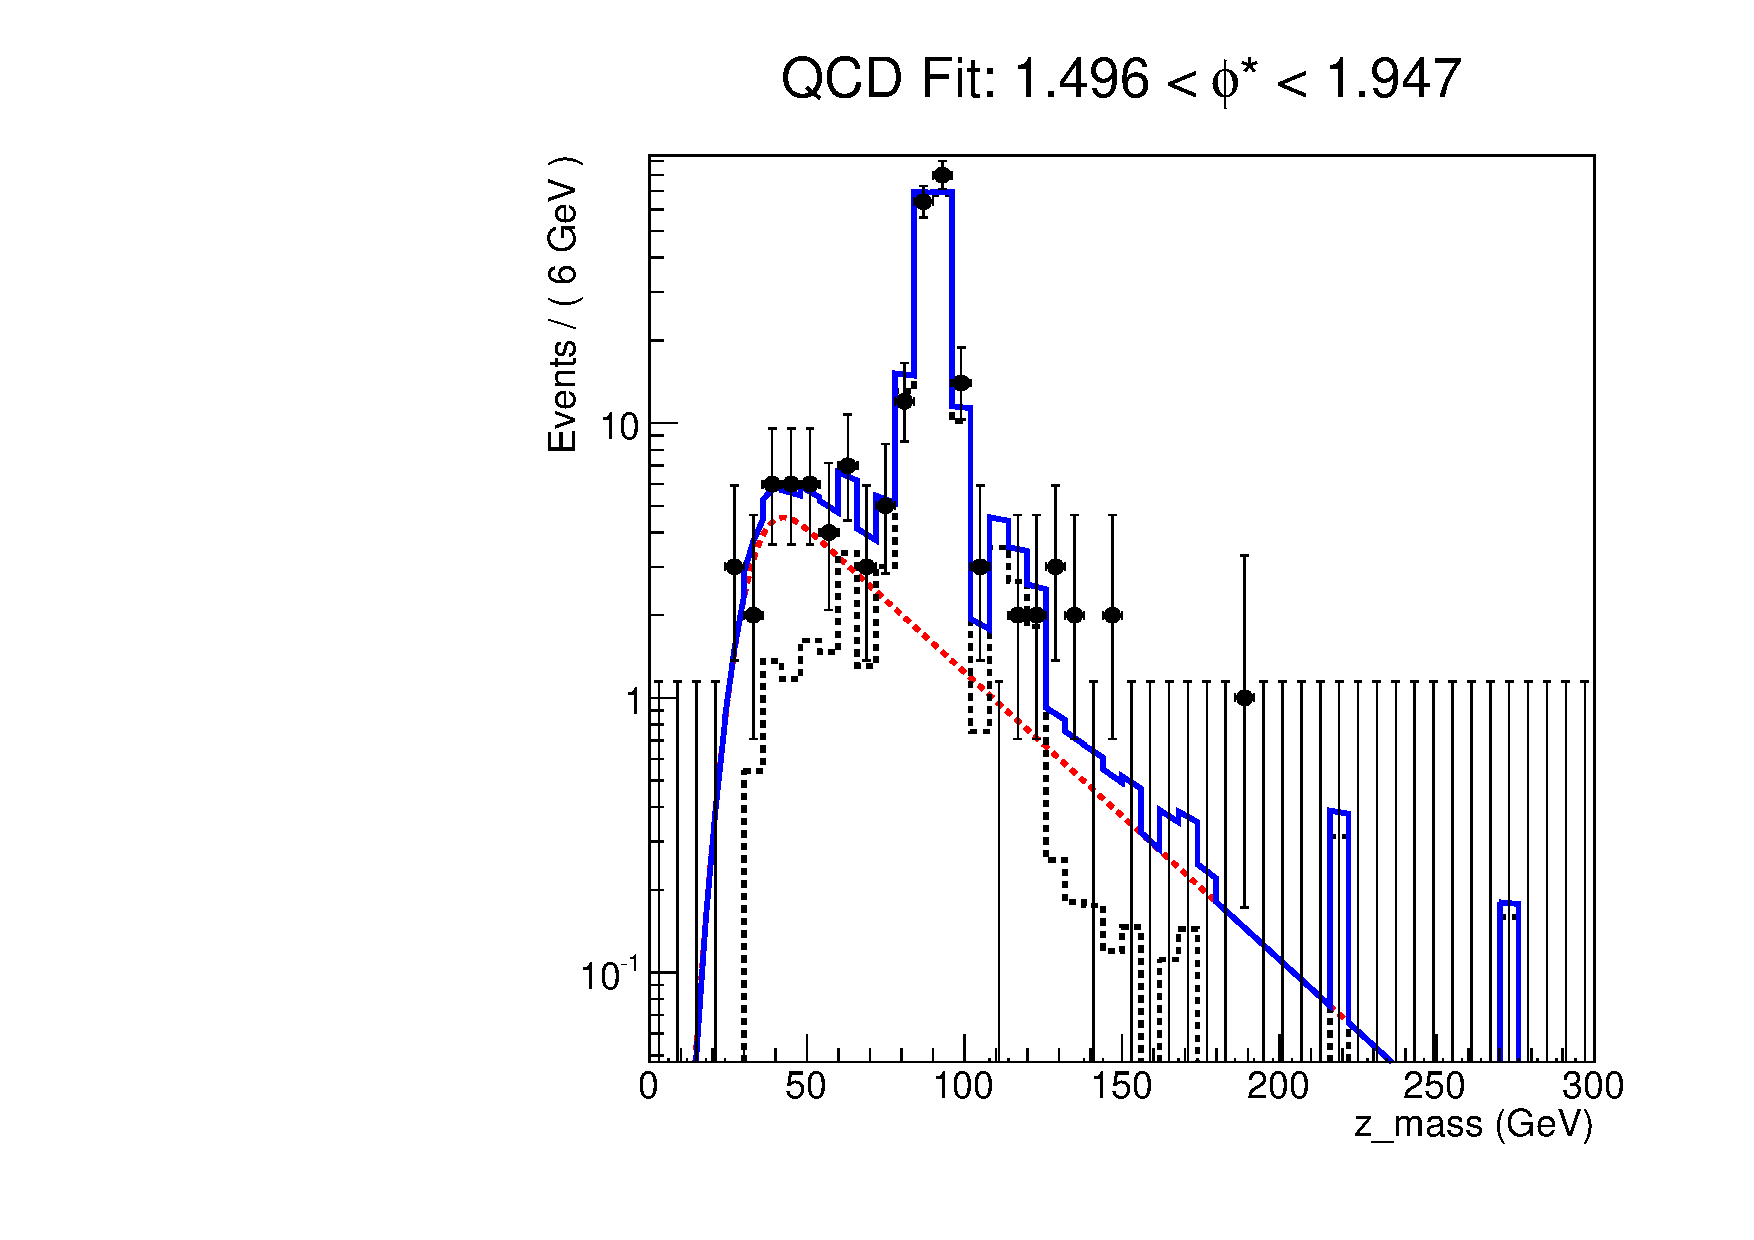
\includegraphics[width=\linewidth]{figures/qcd_fits/qcd_fit_plot_for_32.pdf}
        \label{fig:qcd_fit_32}
    \end{subfigure}
    \caption[
       The \QCDjets and \wjets data-driven background fits for the eighth set
       of four \phistar bins.
    ]{
       The \QCDjets and \wjets data-driven background fits for the eighth set
       of four \phistar bins. The data are shown as points with error bars, MC
       template as a dashed histogram, the analytic background function as the
       dashed line, and the sum of the template and function as a solid
       histogram.
    }
    \label{fig:qcd_many_8}
\end{figure}

\begin{figure}[!htbp]
    \centering
    \begin{subfigure}[b]{\SideBySidePlotWidth}
        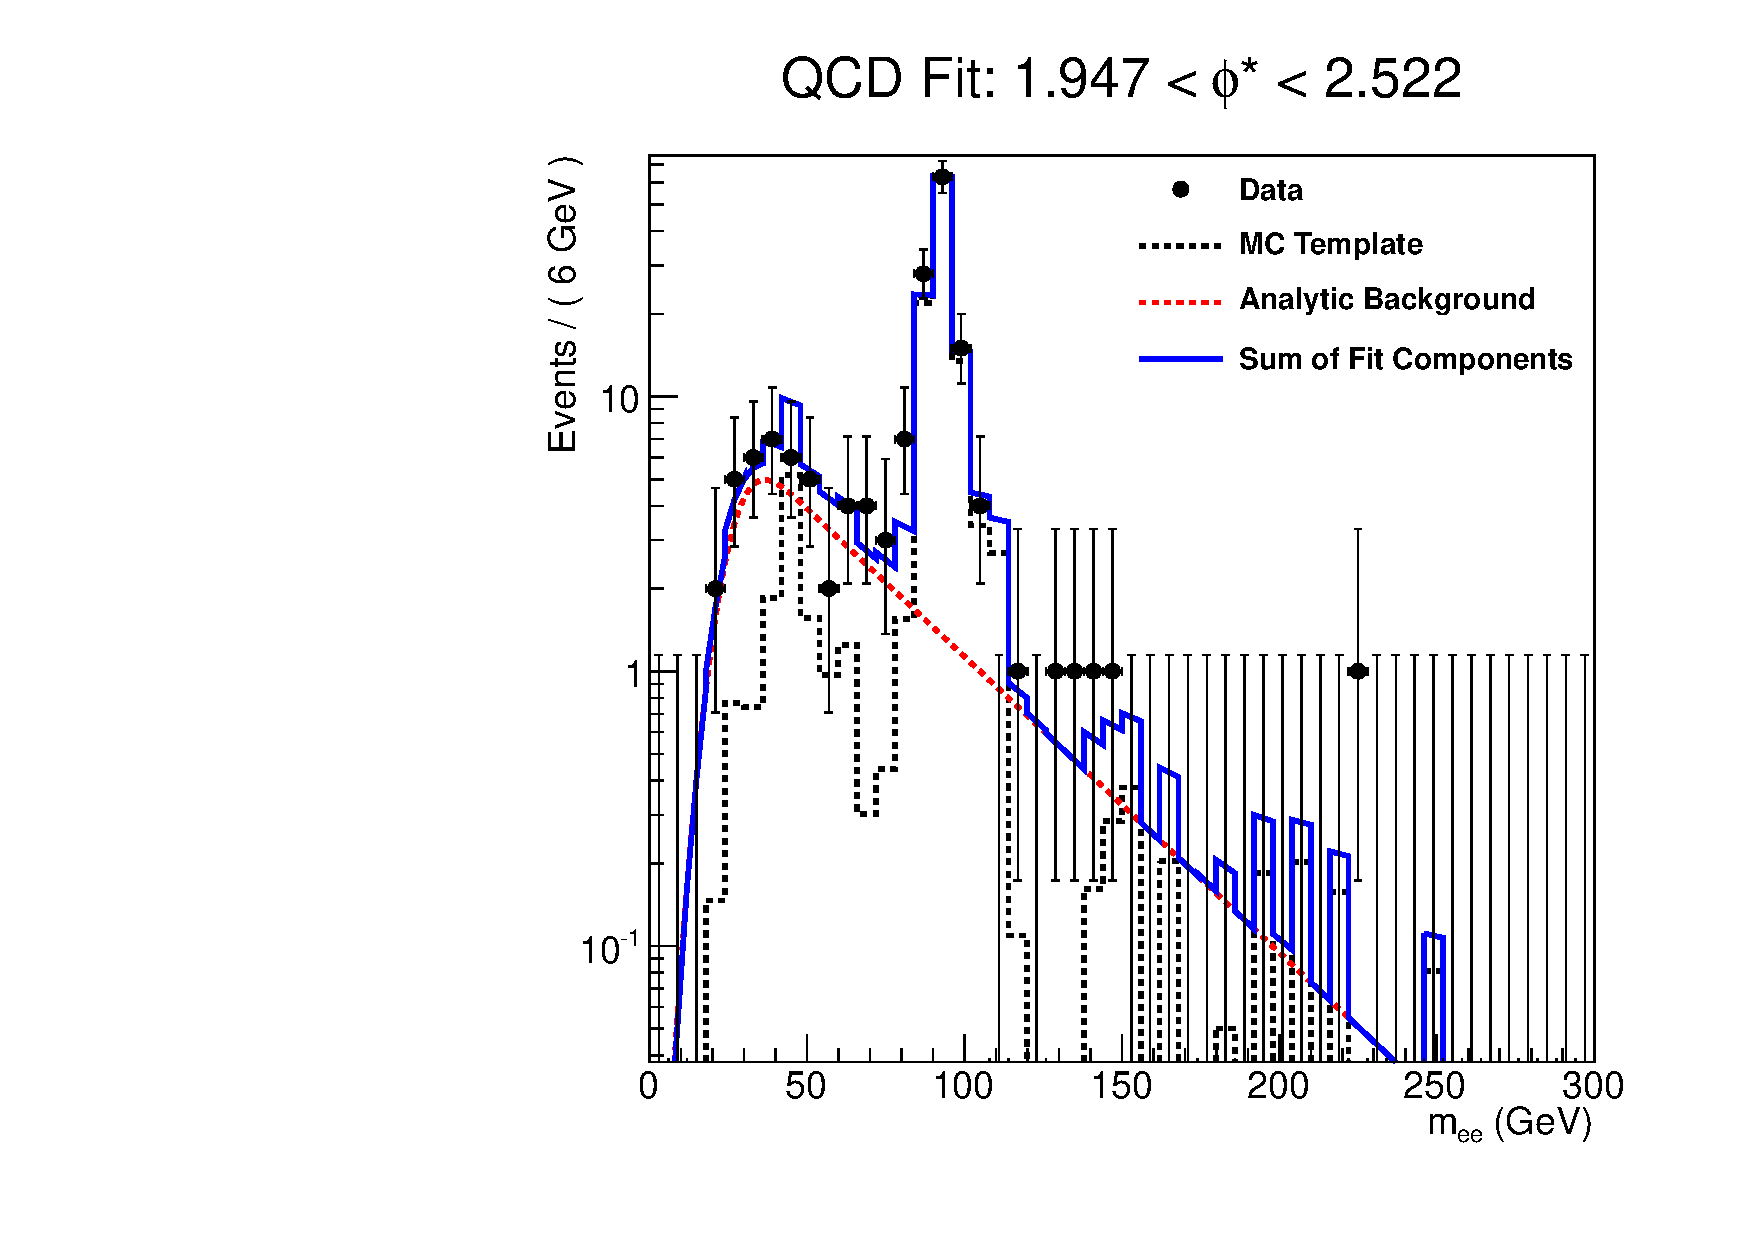
\includegraphics[width=\linewidth]{figures/qcd_fits/qcd_fit_plot_for_33.pdf}
        \label{fig:qcd_fit_33}
    \end{subfigure}%
    % The comment right after suppresses white space that would push the images
    % to new lines
    \begin{subfigure}[b]{\SideBySidePlotWidth}
        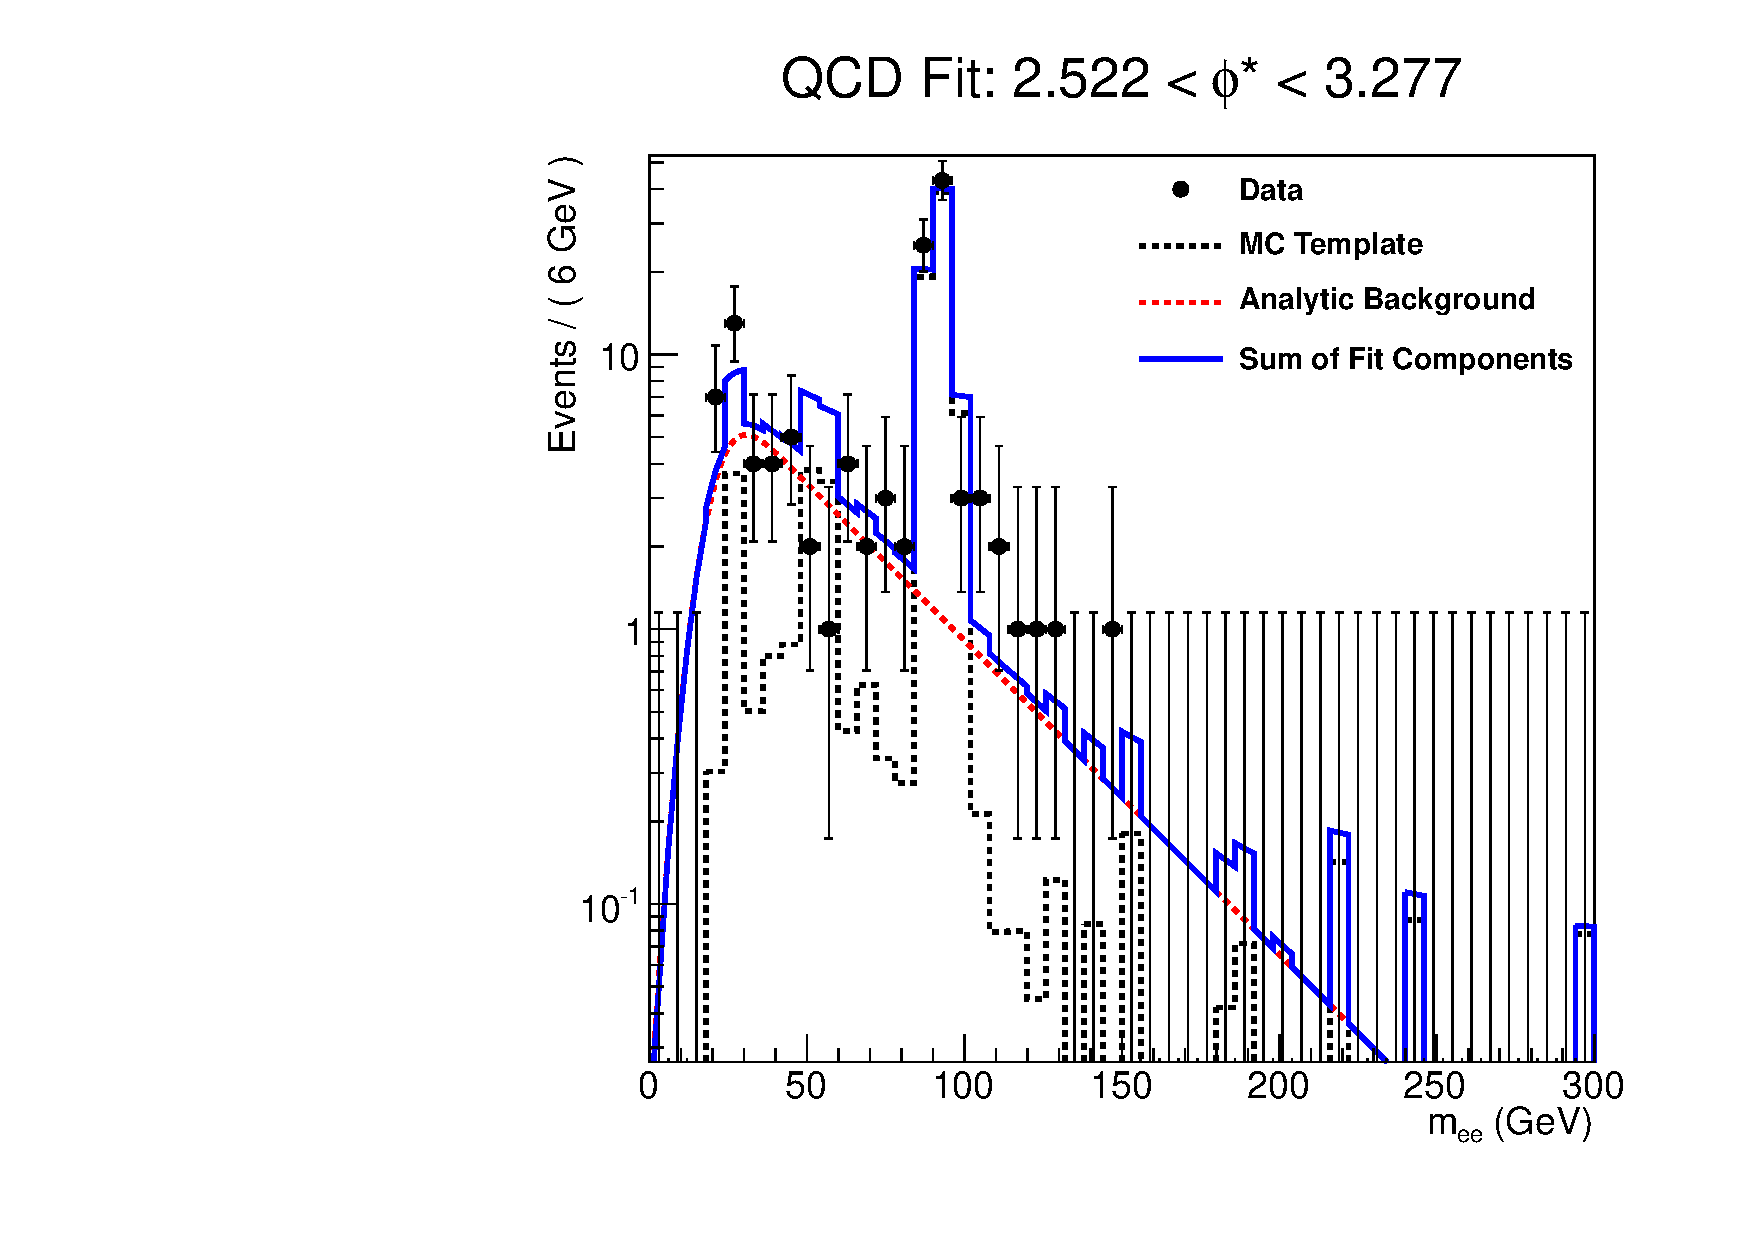
\includegraphics[width=\linewidth]{figures/qcd_fits/qcd_fit_plot_for_34.pdf}
        \label{fig:qcd_fit_34}
    \end{subfigure}
    \caption[
       The \QCDjets and \wjets data-driven background fits for the last two
       \phistar bins.
    ]{
       The \QCDjets and \wjets data-driven background fits for the last two
       \phistar bins. The data are shown as points with error bars, MC template
       as a dashed histogram, the analytic background function as the dashed
       line, and the sum of the template and function as a solid histogram.
    }
    \label{fig:qcd_many_9}
\end{figure}
